%
%
%
\clearpage
\section{Characterization of electromagnetic shower properties with
a Si-Pb sampling calorimeter}
\label{sec:emshowerproperties}

\FIXME{Add introduction}

%%
%%
%%
\subsection{Longitudinal evolution and energy estimation}
\label{subsec:longevol}

In order to characterize the longitudinal evolution of the showers in
our setup we count the total energy deposited by all hits in the Si layers. 
Energy is measured relatively to the estimated MIP signal (see details
ahead in Sec.~\ref{sec:digi}).
In this study electron events are used: for incoming energies
below 150\GeV, 2500 events have been generated; for higher energies
1250 events are used.

Figure~\ref{fig:showerfits} shows the longitudinal shower evolution
for single electron events as function of the \Xnot transversed in the
detector.
It can be observed that the level of energy fluctuations for low
energetic electrons is non-negligible, with $\delta$ deposits
dominating the contribution to the total energy deposited in each Si
layer.
For sufficiently energetic electrons these contributions become of
second order and the characterization of the shower is dominated by
the statistical fluctuations in the number of particles comprising the shower.
For very high energy showers ($>$150\GeV) part of the energy can't be
contained in the detector setup using 25\Xnot. Given that in this
regime the showers are dominated by statistical fluctuations in its
composition a fit to the longitudinal profile can be used safely and
used to estimate the leakage fraction.

\begin{figure}[h!]
  \begin{center}
    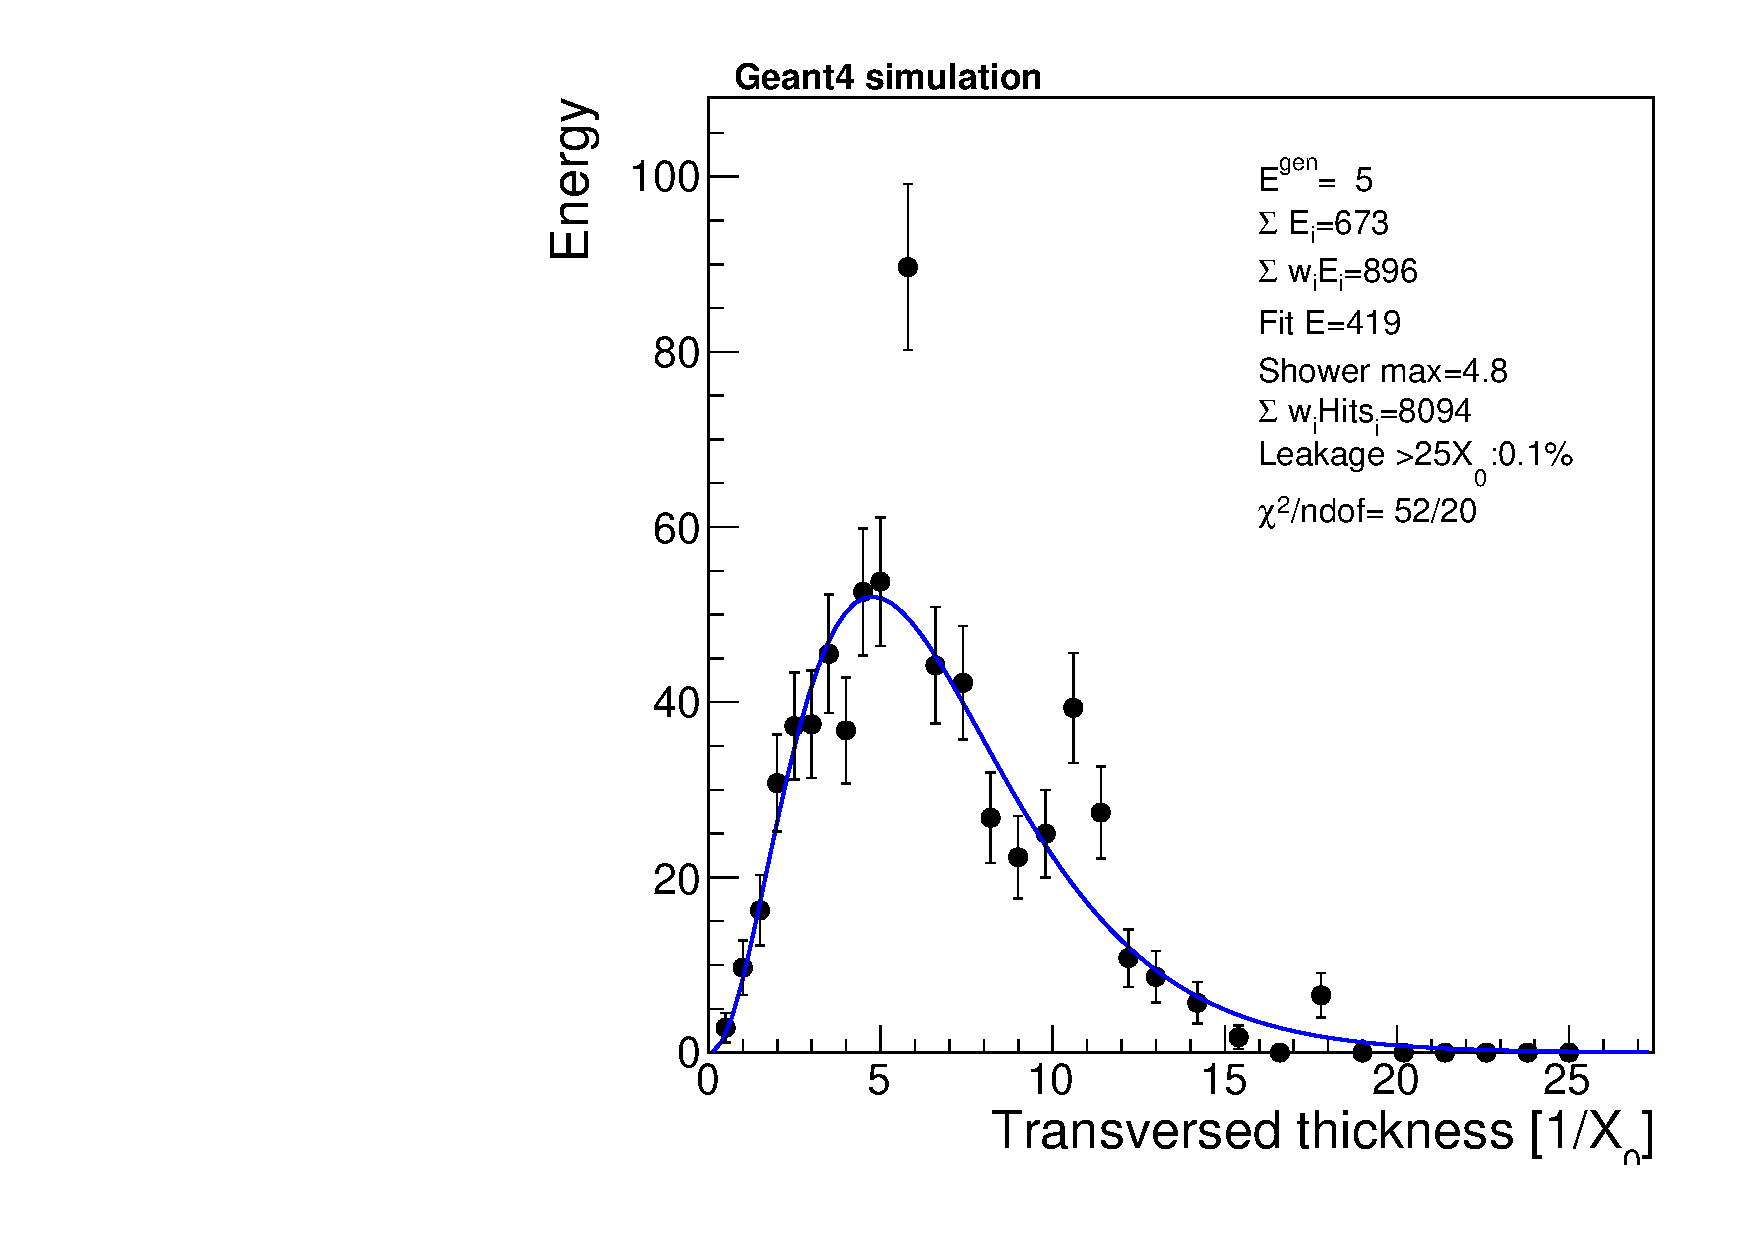
\includegraphics[width=0.24\textwidth]{figures/version_3e_5_5_showerfits}
    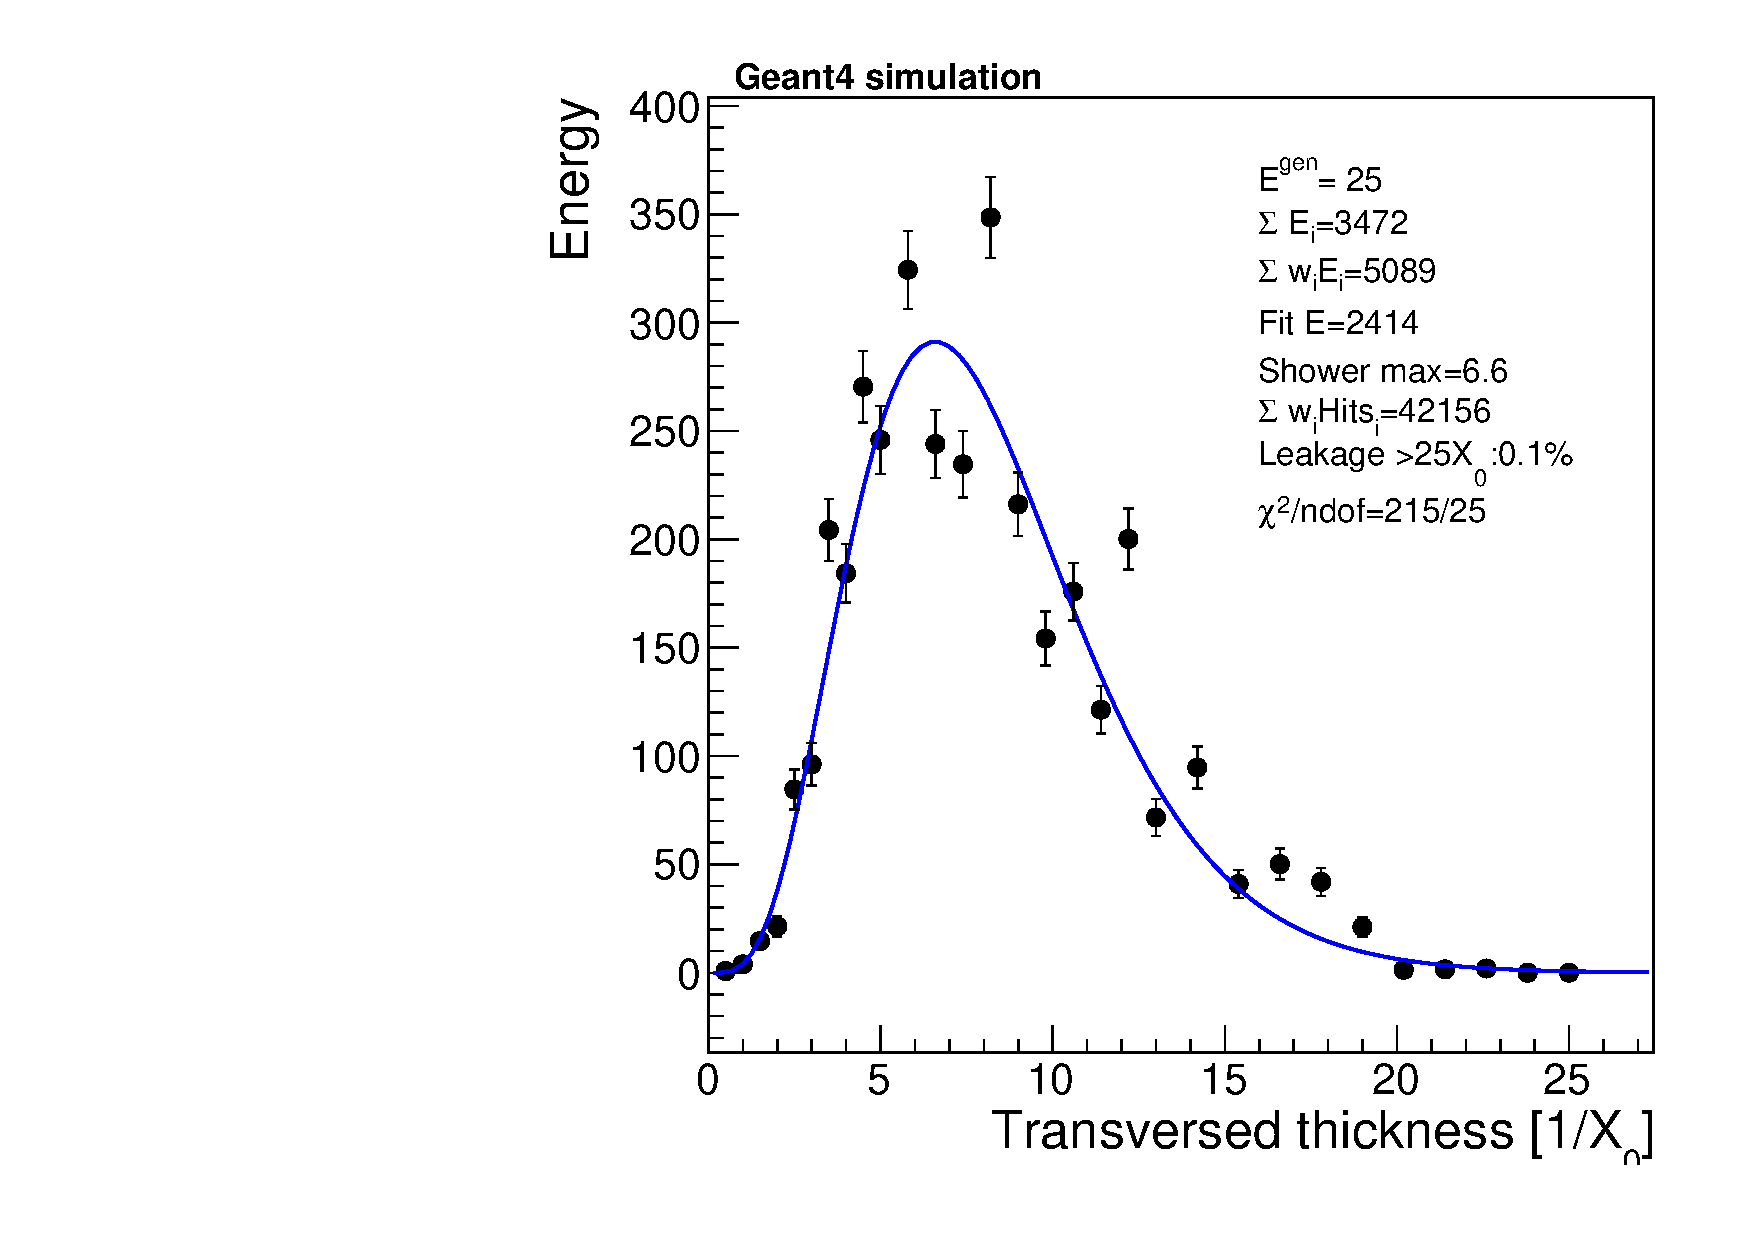
\includegraphics[width=0.24\textwidth]{figures/version_3e_25_8_showerfits}
    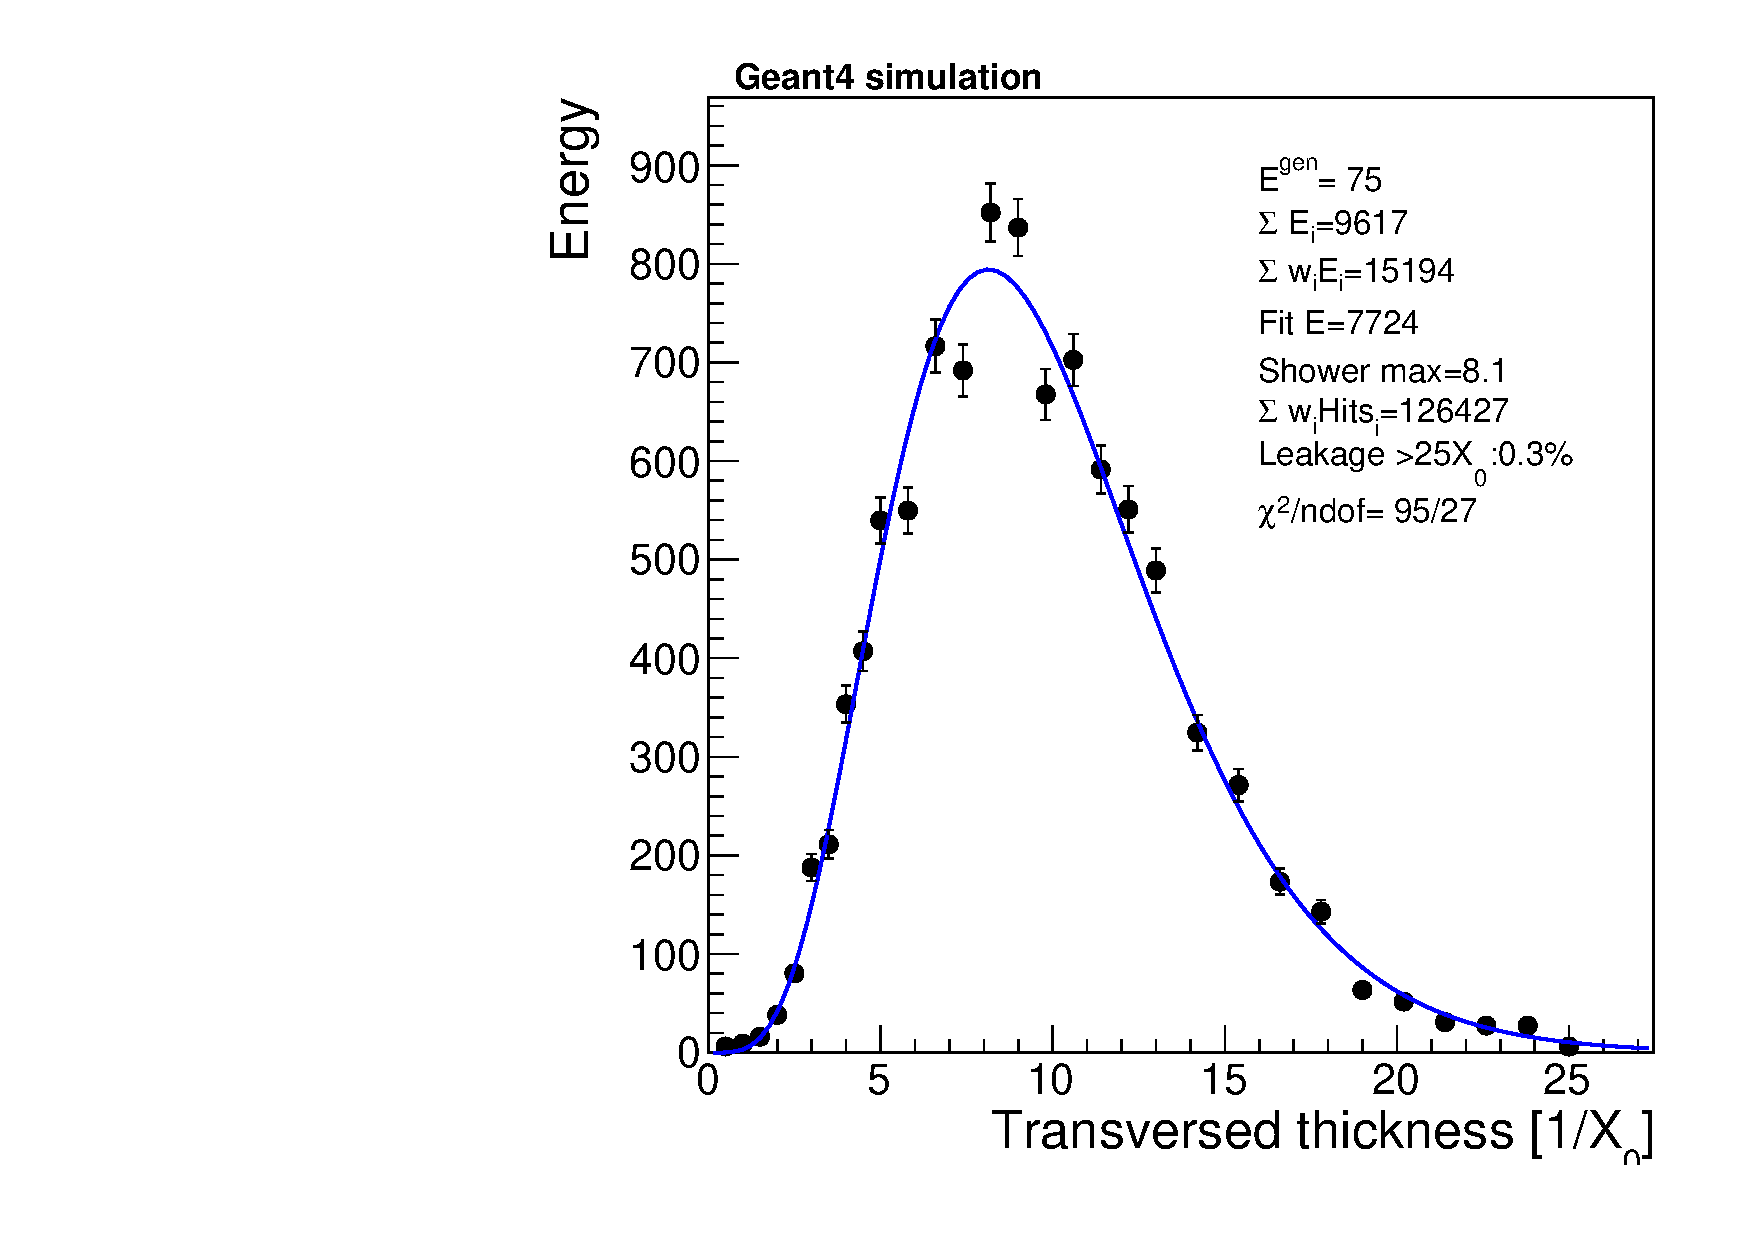
\includegraphics[width=0.24\textwidth]{figures/version_3e_75_6_showerfits}
    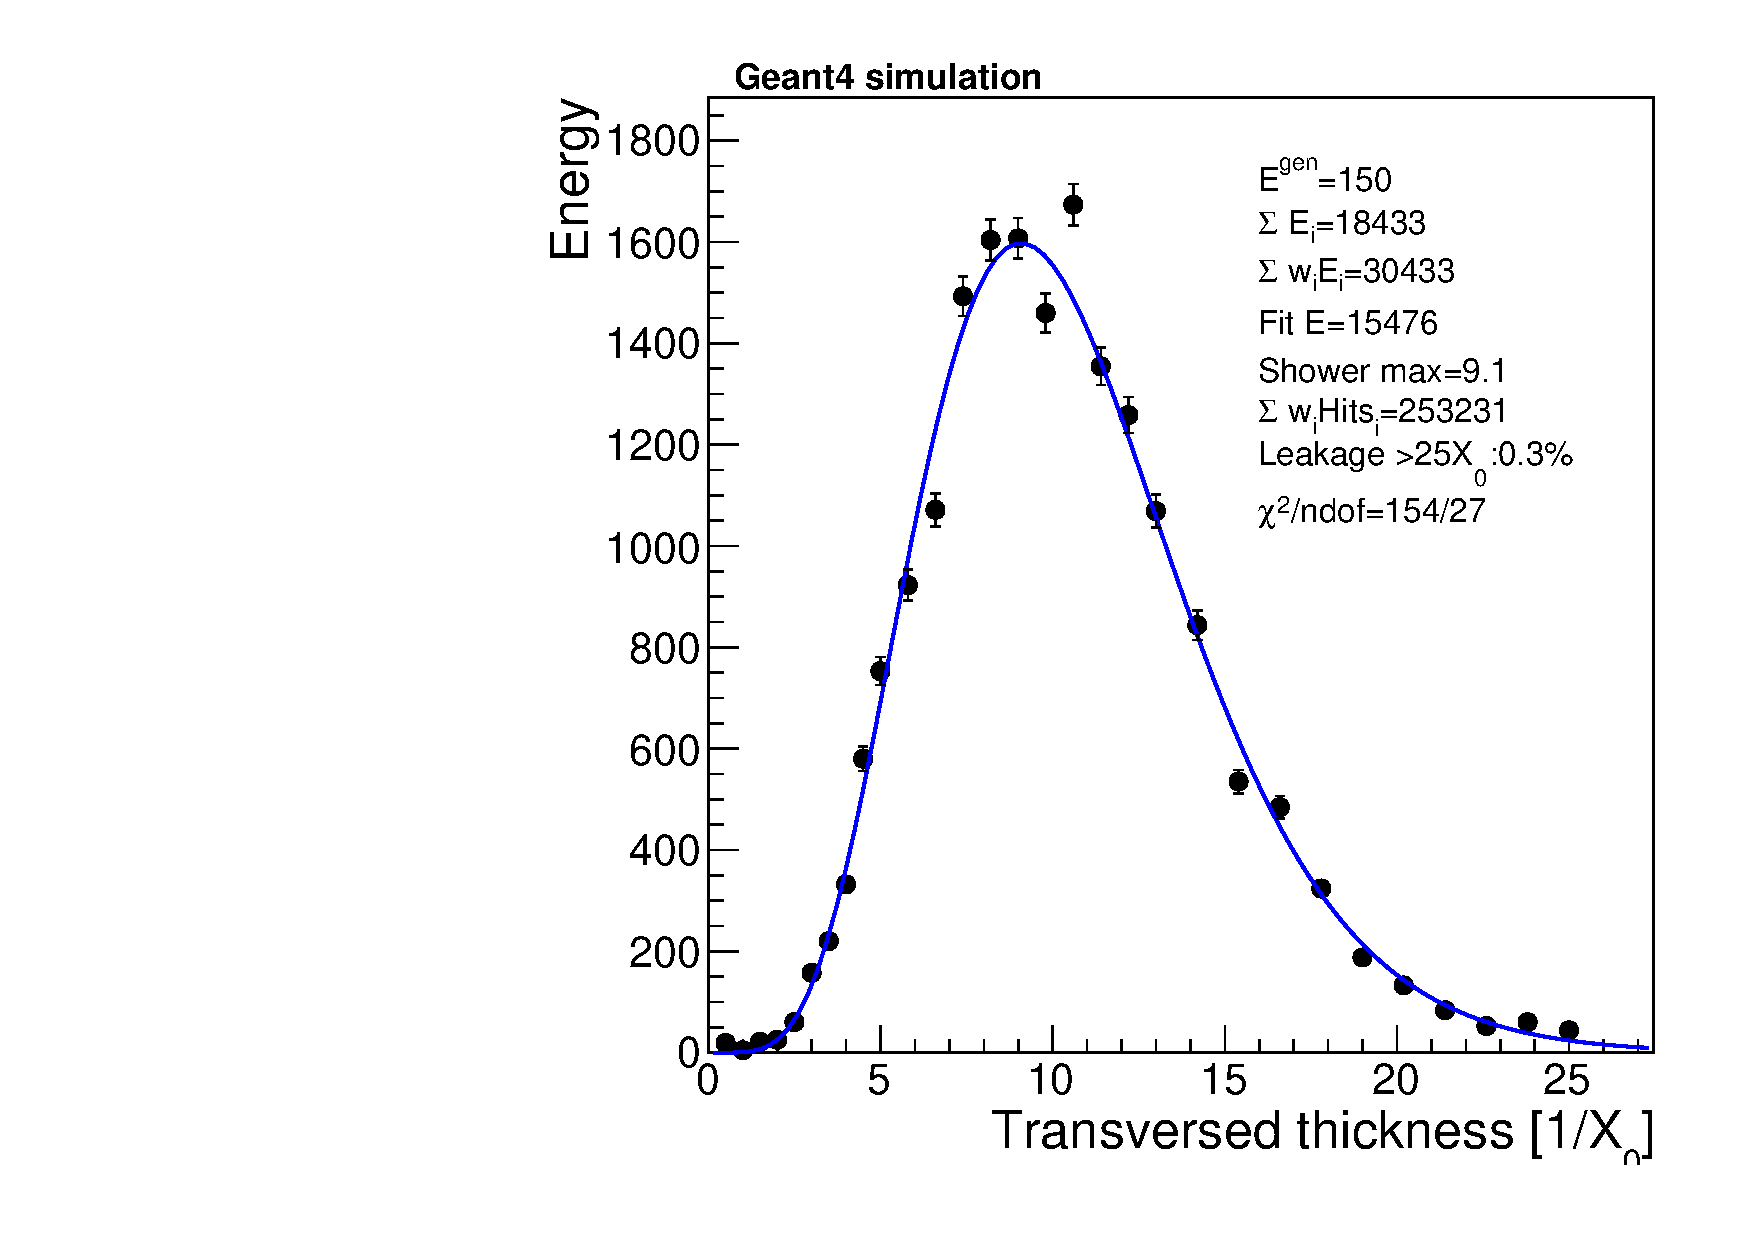
\includegraphics[width=0.24\textwidth]{figures/version_3e_150_6_showerfits}
    \caption{From {\em left} to {\em right}: energy deposits in different Si layers for single
      electron events with energies: 10, 25, 50, 100\GeV. The deposits
    are shown as function of the transversed distance in \Xnot
    units. A fit is overlaid using the functional form described in
    the text. 
     The results obtained for the different energy estimators
     considered in the analysis, as well as for the shower leakage
     estimated from the fit, are shown in the caption}
    \label{fig:showerfits}
  \end{center}
\end{figure}

Thus, different methods to estimate the total energy of the shower are
compared:

\begin{description}

\item[Raw energy] we sum inclusively of all the energy deposited in
  the Si layers assuming the full sensitive area volume;

\item[Weighted energy] we sum the energy deposited in each Si layer
  normalized by the material overburden of the sampling section,\ie:

\begin{equation}
{\rm weighted~E}=\sum_{i=1}^{N} \frac{X_0^i}{X_0^1}\cdot E_i
\label{eq:weightenest}
\end{equation}

For the baseline setup these weights correspond to 1 for section A,
1.6 for section B and 2.4 for section B.
These weights can also be optimised to minimise the energy resolution
for the incoming energy range of interest.

\item[Shower profile fit] - a functional form is used to adjust the
  measured energy deposits in each layer:

\begin{equation}
\mathcal{E}(x)=\alpha\cdot x^{a} \cdot e^{-bx} 
\label{eq:showerprof}
\end{equation}

where x is the transversed material overburden measured in \Xnot
units. This approach is expected to recover the shower leakage for
higher incident energies.

\item[Shower maximum] - the position of the shower max can be used as a
  coarse estimator for the energy. It can be estimated after the
  shower fit by the ratio $X_{0}^{\max}=b/a$.

\item[Hit counting] - this estimator, altough impossible to be used in
  reality, is used to gauge to potential of the setup. We use the
  weighted sum  of the number of hits generated per Si layer as an
  estimator of the initial energy. The weights are the same as define
  in Eq.~\ref{eq:weightenest}.

\end{description}

For each method the distribution of the estimator is fitted with a
gaussian for each incoming generated beam energy. An unbinned-likelihood fit is
used for this purpose. Figures~\ref{fig:fithitcount}
and~\ref{fig:fitwen}
show two examples using the weighted energy and the hit counting
estimators correspondingly.

\begin{figure}[h!]
  \begin{center}
    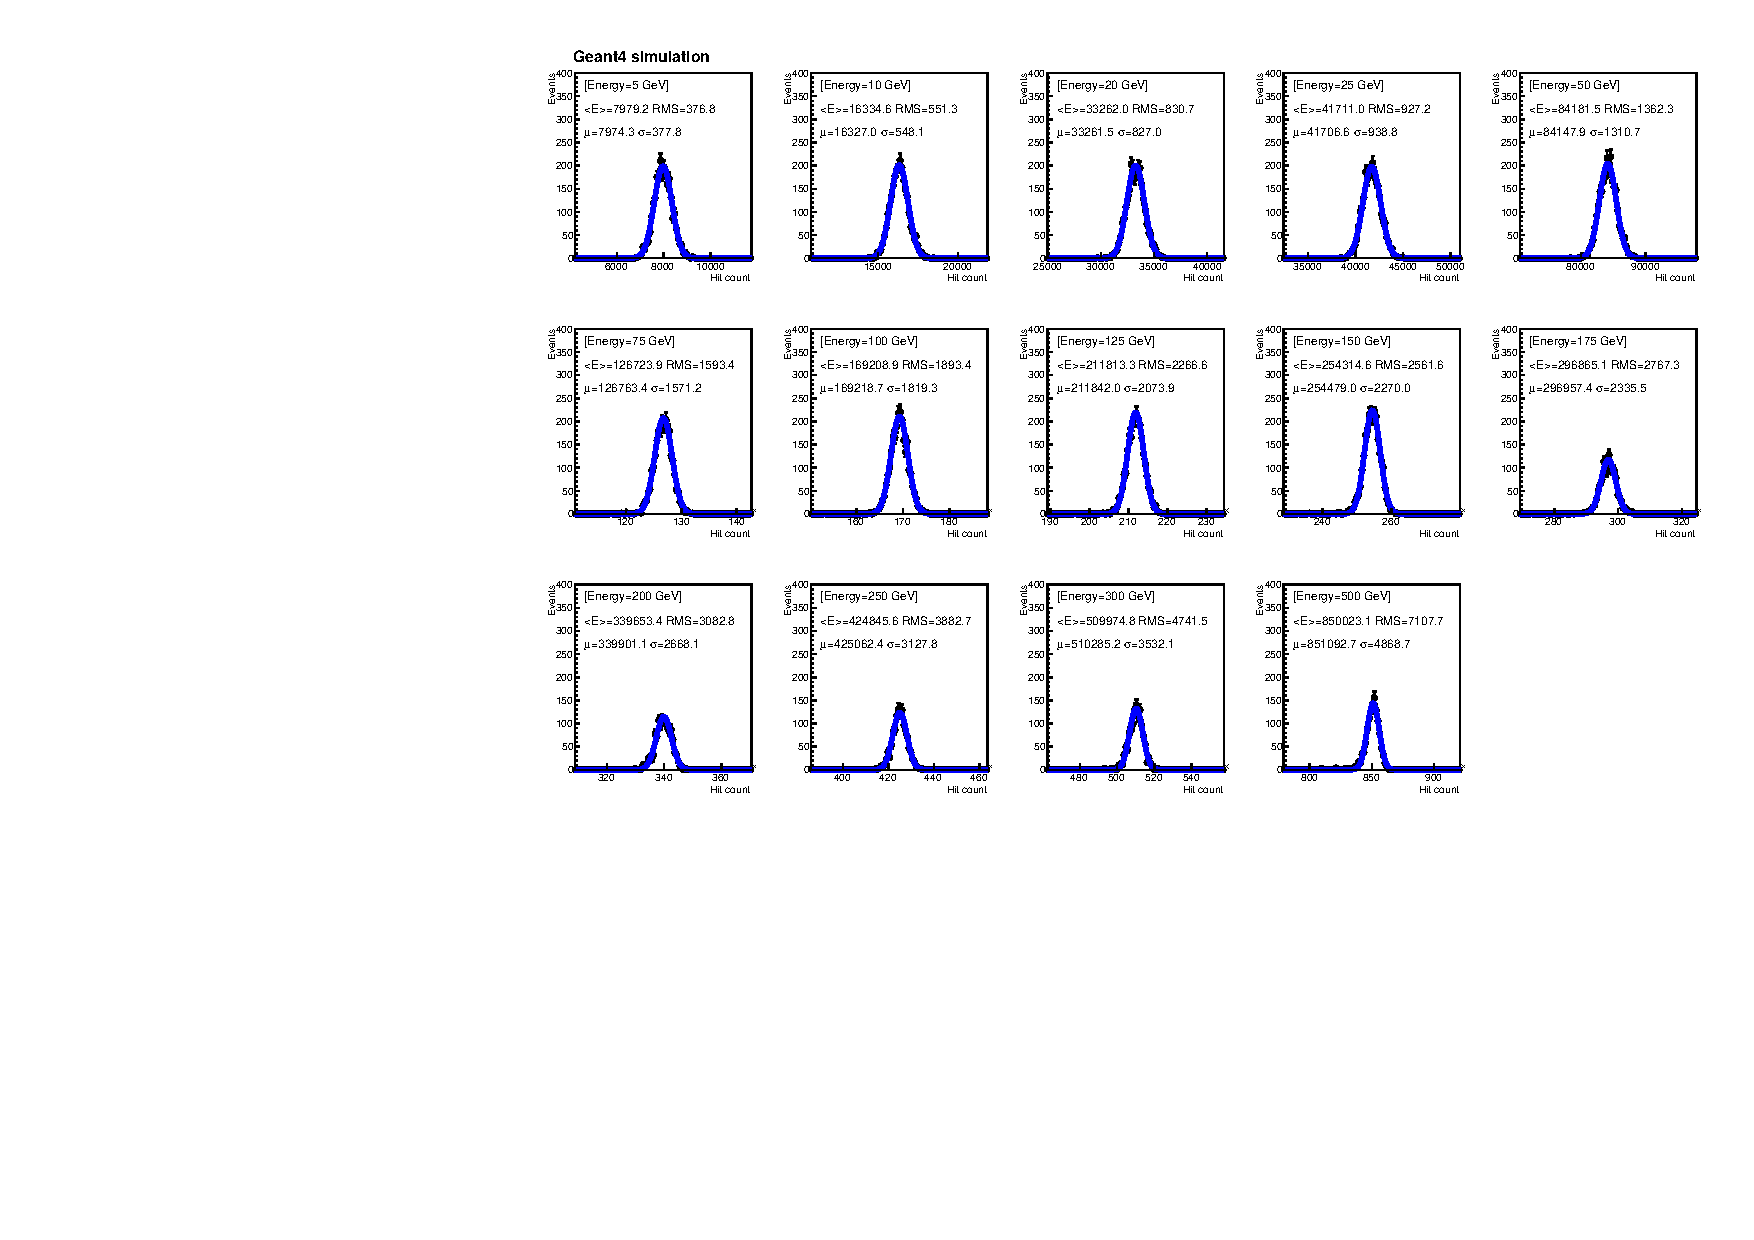
\includegraphics[width=0.99\textwidth]{figures/recenergy_nemHits}
    \caption{Weighted energy sum estimator distributions for different
    beam energies. The result of an unbinned-likelihood fit of a gaussian is
    superimposed. The mean and average of the distribution and the
    gaussian are compared in the caption.}
    \label{fig:fithitcount}
  \end{center}
\end{figure}

\begin{figure}[h!]
  \begin{center}
    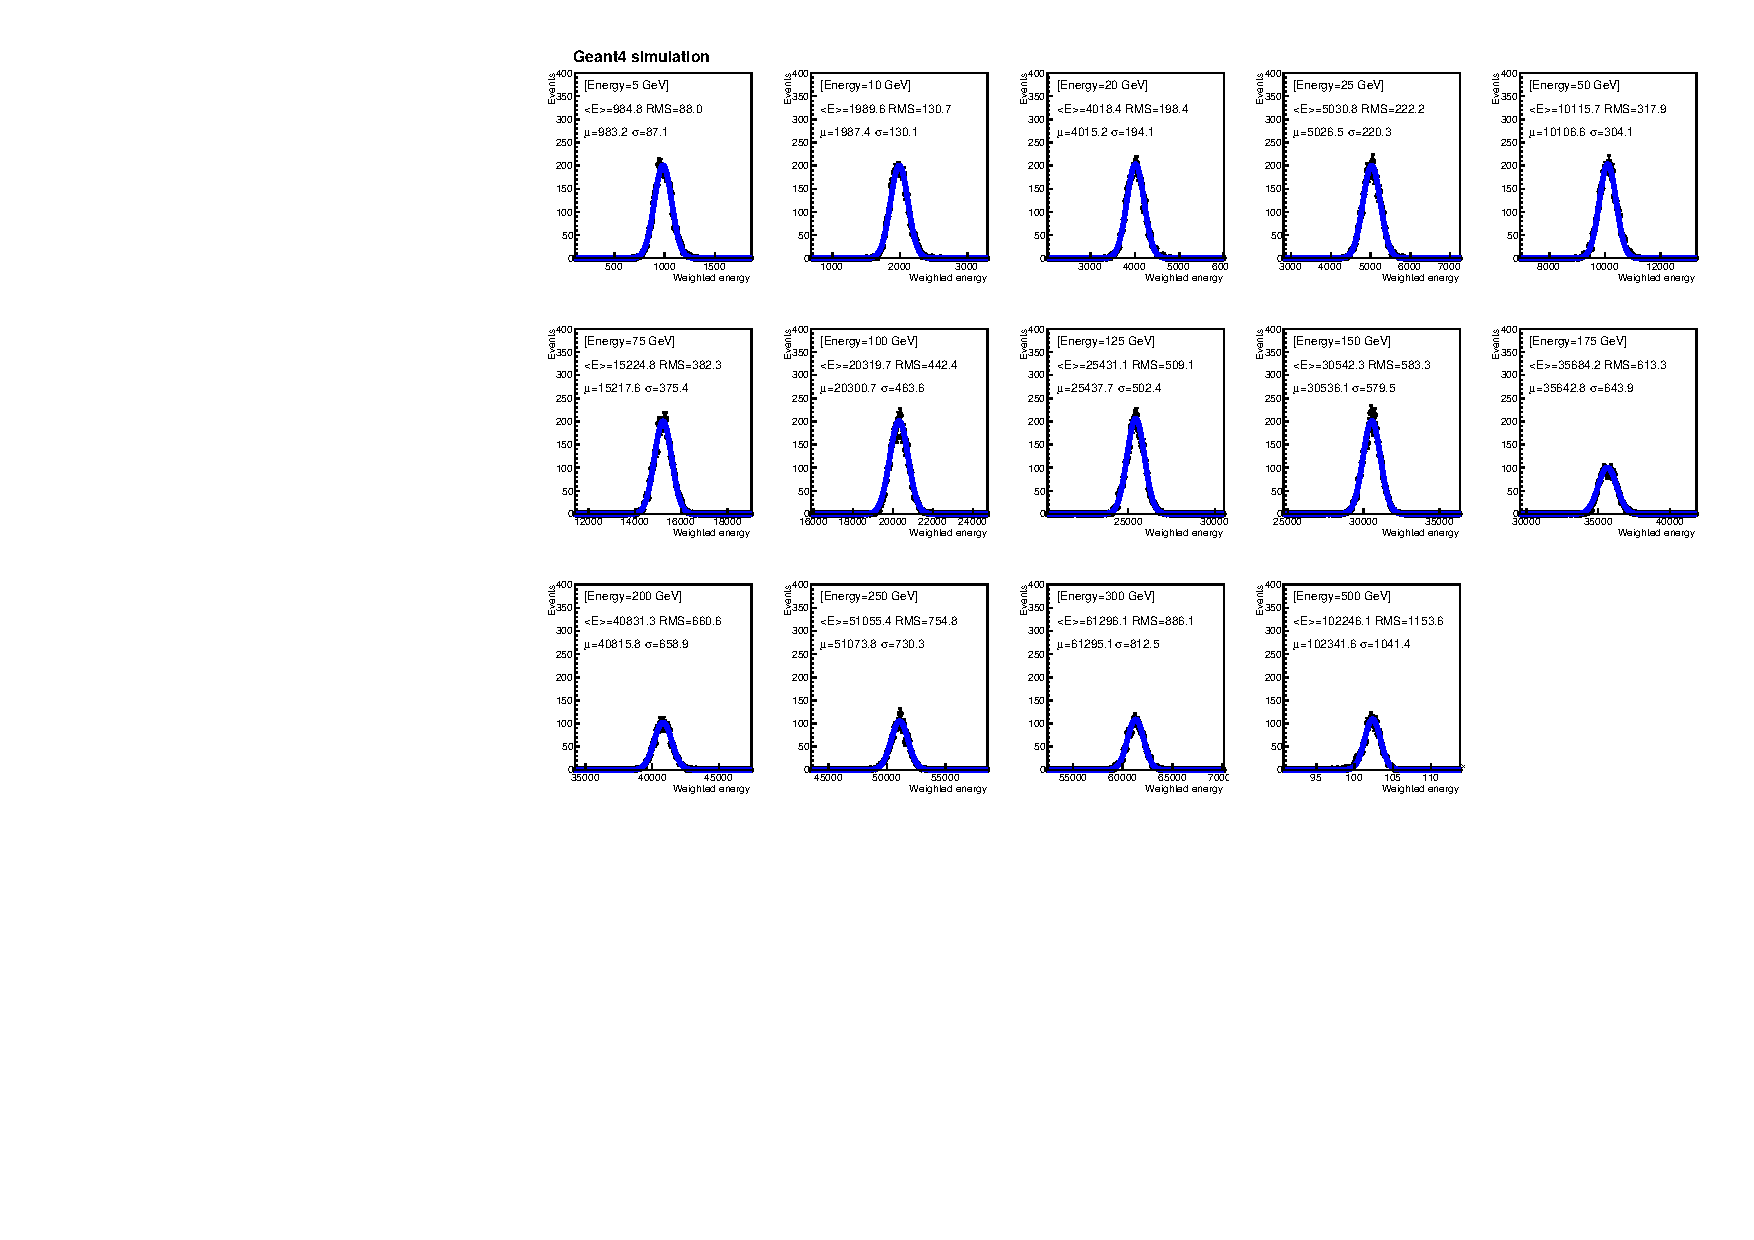
\includegraphics[width=0.99\textwidth]{figures/recenergy_sumWEn}
    \caption{Similar to Fig.~\ref{fig:fithitcount} for the weighted energy sum estimator.}
    \label{fig:fitwen}
  \end{center}
\end{figure}

The parameters of the fitted gaussians can be used for two purposes:
the mean is used to obtain the calibration (\ie dependency of the
energy estimator on the incoming energy) and the ratio of the width
with respect to the mean as an estimator for the resolution.
The calibration curves obtained are shown in Fig.~\ref{fig:baselinelinandresol}
{\em left} where linear behaviour is observed for all the estimators.
Figure~\ref{fig:baselinelinandresol} {\em right} shows the energy
resolution as a function of the incoming energy. 
A fit to a resolution model is super-imposed for each curve. The
resolution model is based on the quadratic sum of a stochastic term
(proportional to $1/\sqrt{E}$) with a constant term,\ie:

\begin{equation}
\left(\frac{\sigma_{\rm E}}{\rm E}\right)^2 = \left(\frac{\sigma_{\rm
      stoch}}{\sqrt{\rm E}}\right)^2+\sigma_{\rm cte}^2
\label{eq:resmodel}
\end{equation}

As expected, altough the raw energy estimator scales faster with
energy (\ie has smaller stochastic term) its resolution fastly
saturates at a non-negligible due to the fact that the sampling is
non-uniform. The weighted energy estimator is able to recover from
this attaining a baseline resolution of the order of 20.9\%. The
residual constant term can be almost fully removed with a shower
leakage recovery algorithm such as the one provided by the fitted
energy estimator - in this approach the constant term is observed to
be compatible with 0.
The hit count approach yields the best resolution expected to be
attainable with this setup. The shower max estimator has worse
resolution and large constant term.

\begin{figure}[h!]
  \begin{center}
   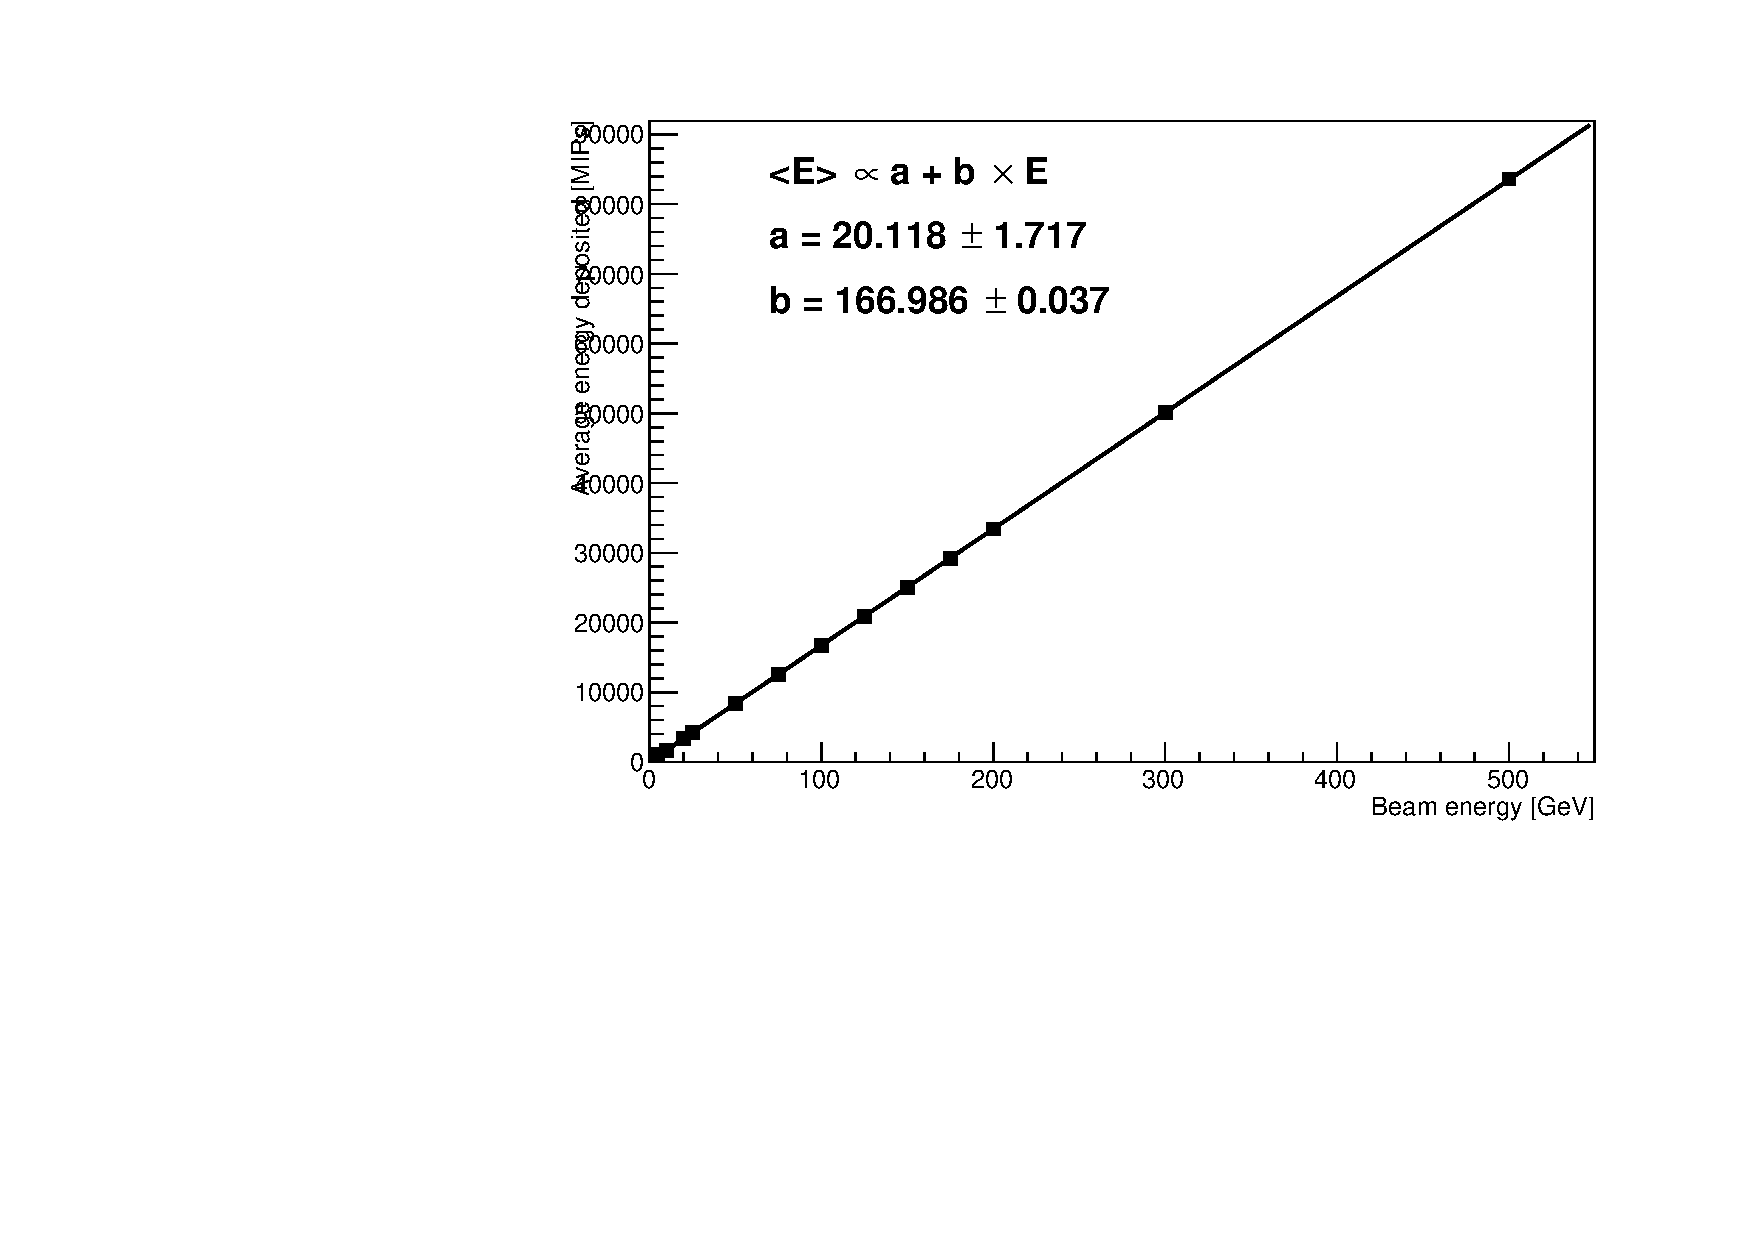
\includegraphics[width=0.48\textwidth]{figures/e_calibFit}
    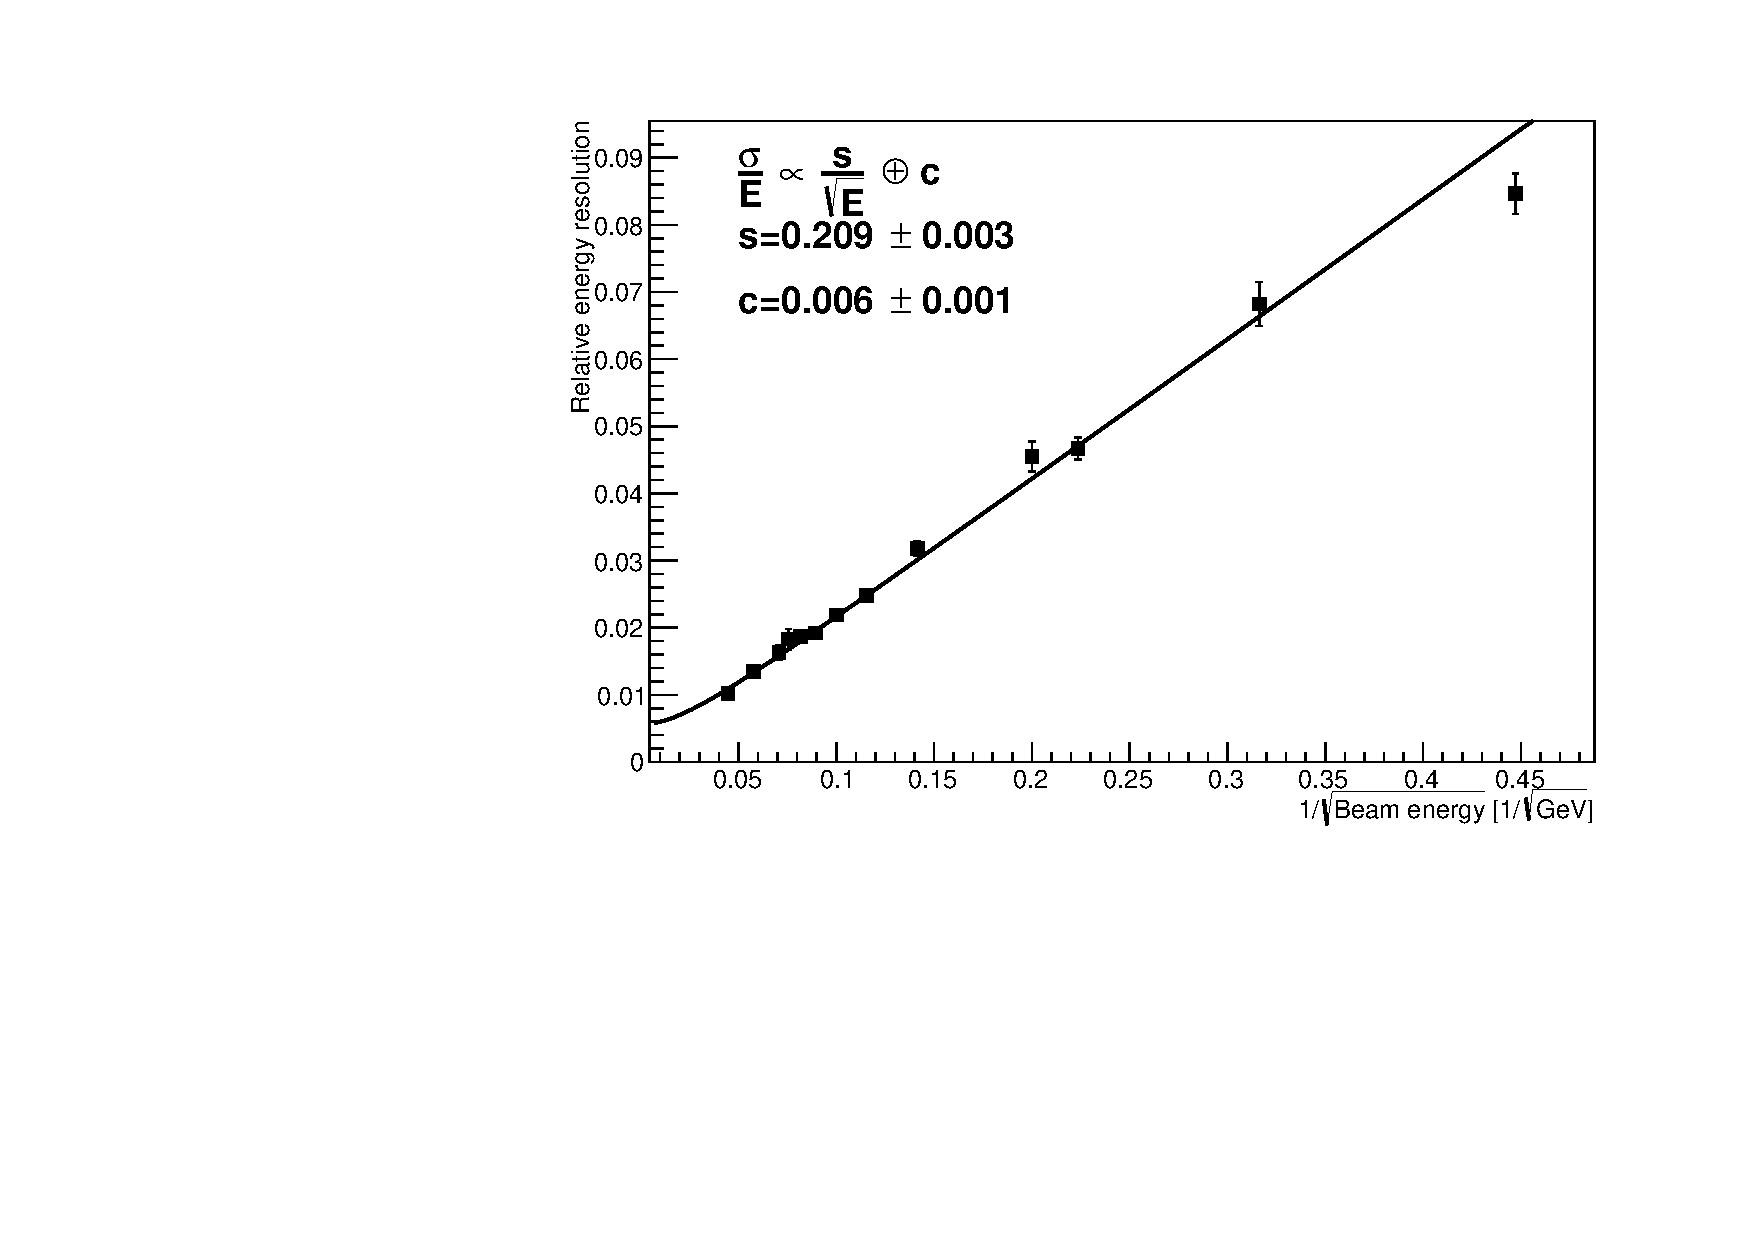
\includegraphics[width=0.48\textwidth]{figures/e_resoFit}
    \caption{{\em Left}: reconstructed energy (in MIP units) as a function of the generated
      energy E. {\em Right}: energy resolution as a function of
      $\frac{1}{\sqrt{E}}$. In both cases single electron events are simulated.}
    \label{fig:baselinelinandresol}
  \end{center}
\end{figure}


Figure~\ref{fig:longenergydep} shows the energy deposits distribution
as function of the distance to the estimated shower maximum for
different incident energies. The shower maximum is estimated on an
event by-event-basis using the procedure described above.
These distributions can be used to
profile both the average energy deposit 
as well as the characteristic spread at each layer (or shower age).

\begin{figure}[h!]
  \begin{center}
   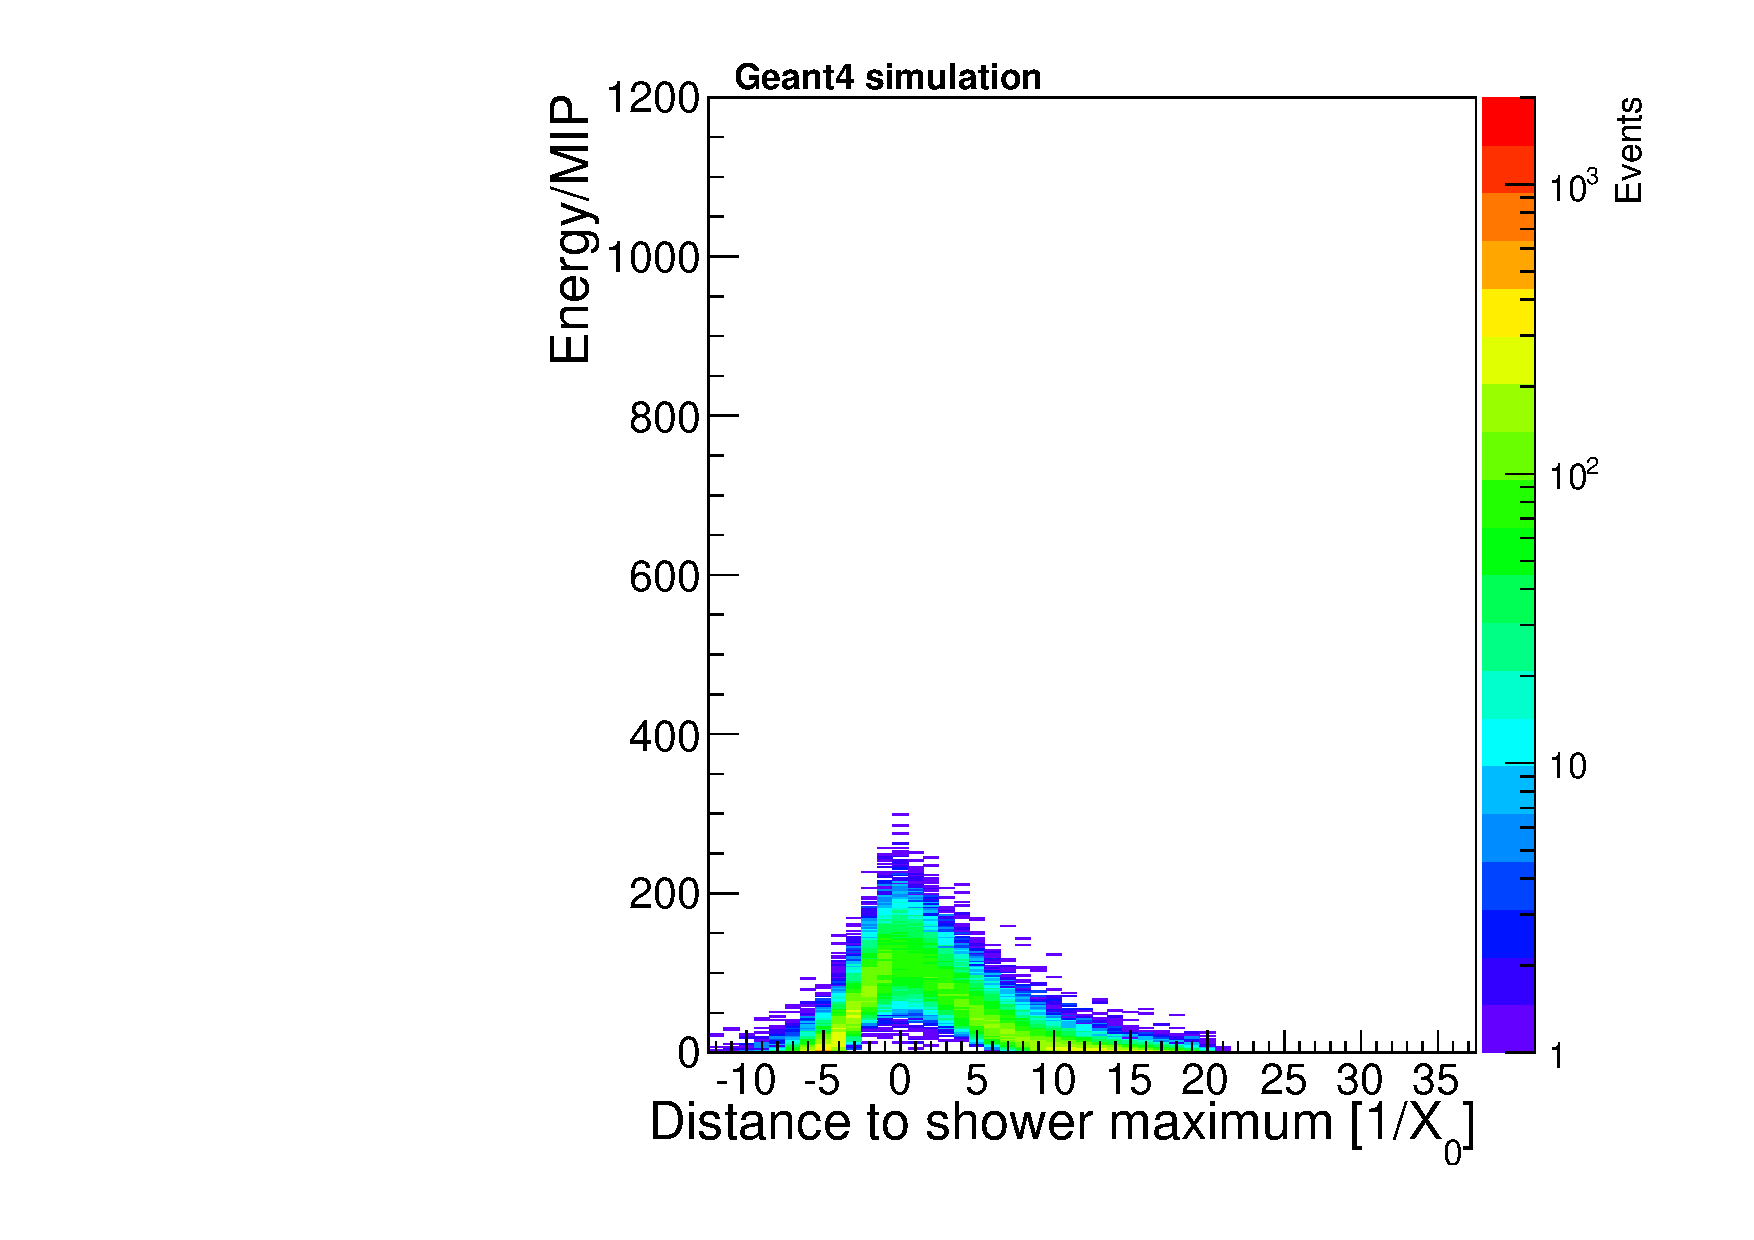
\includegraphics[width=0.23\textwidth]{figures/version_3e_10_showerprof}
    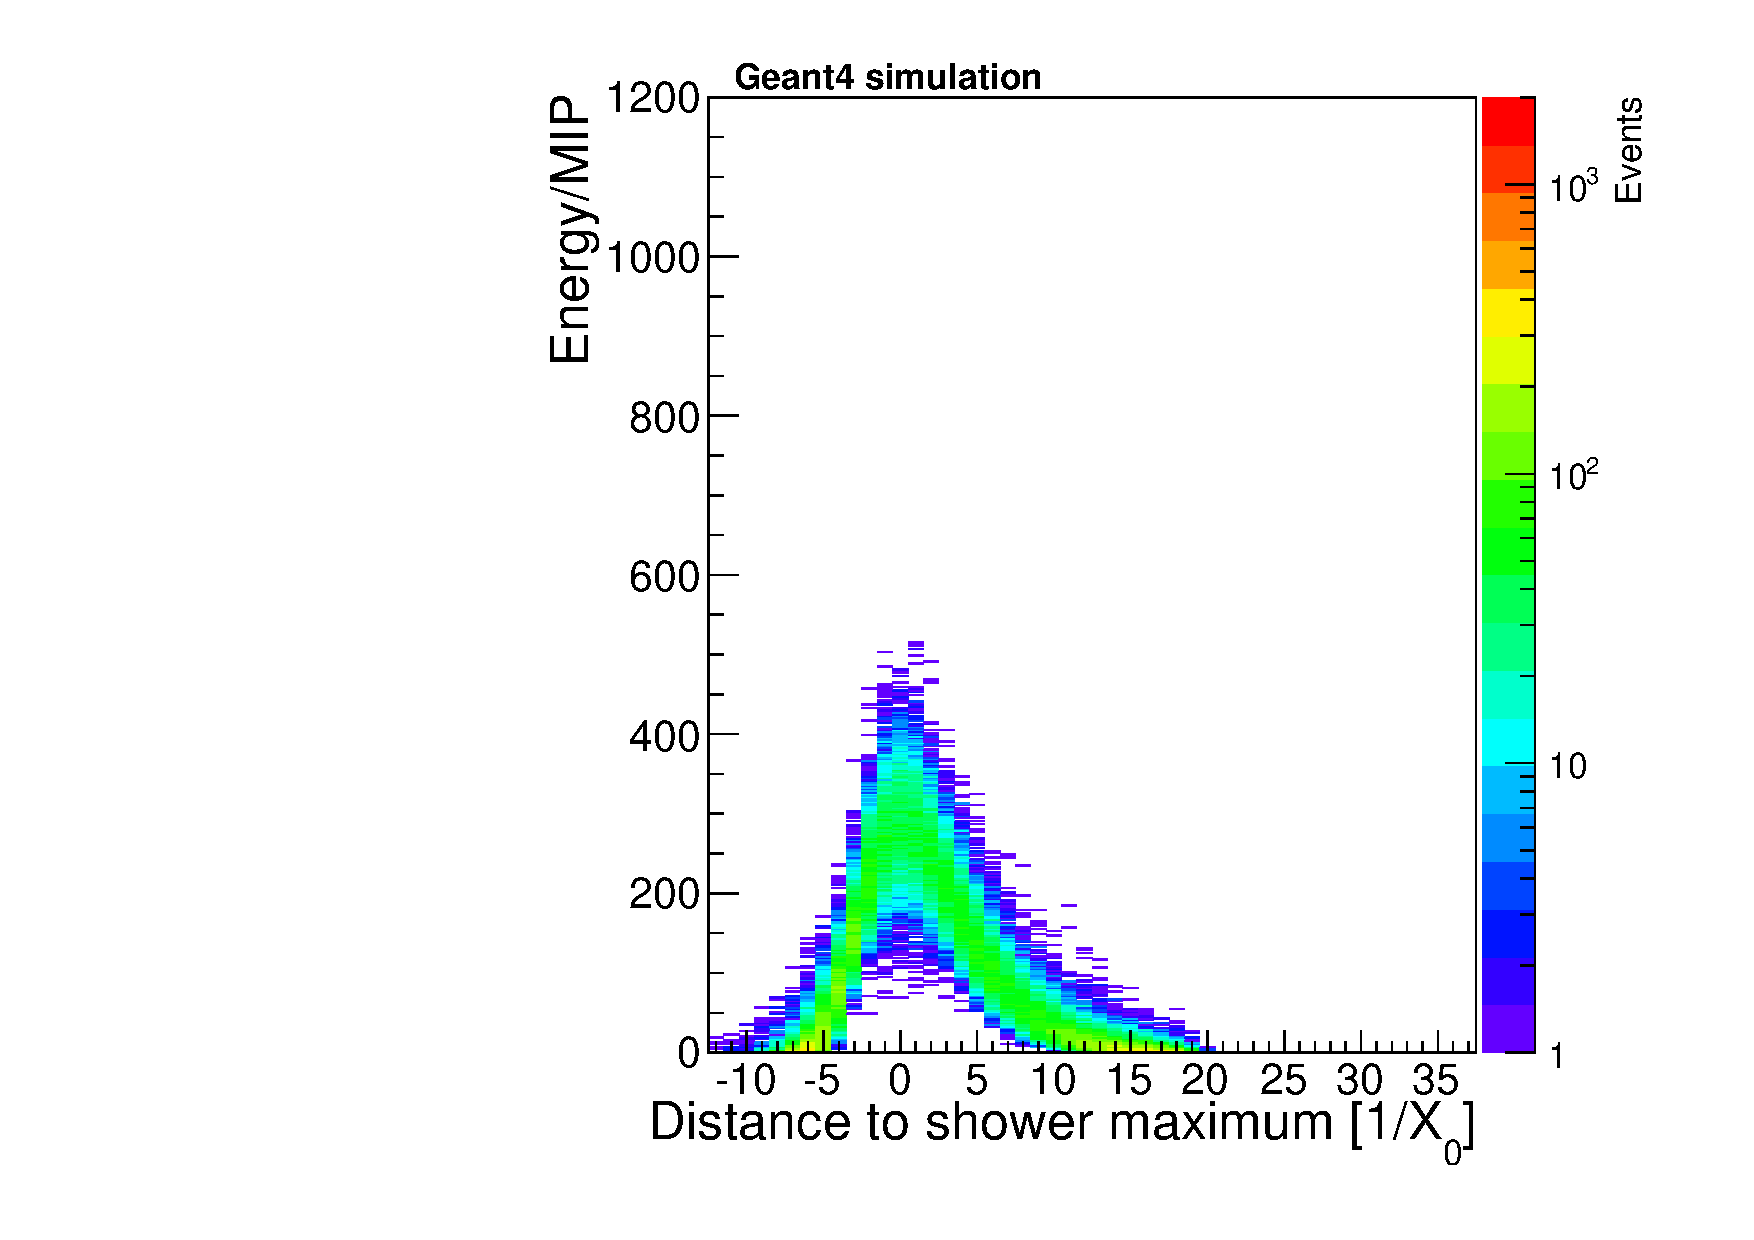
\includegraphics[width=0.23\textwidth]{figures/version_3e_25_showerprof}
    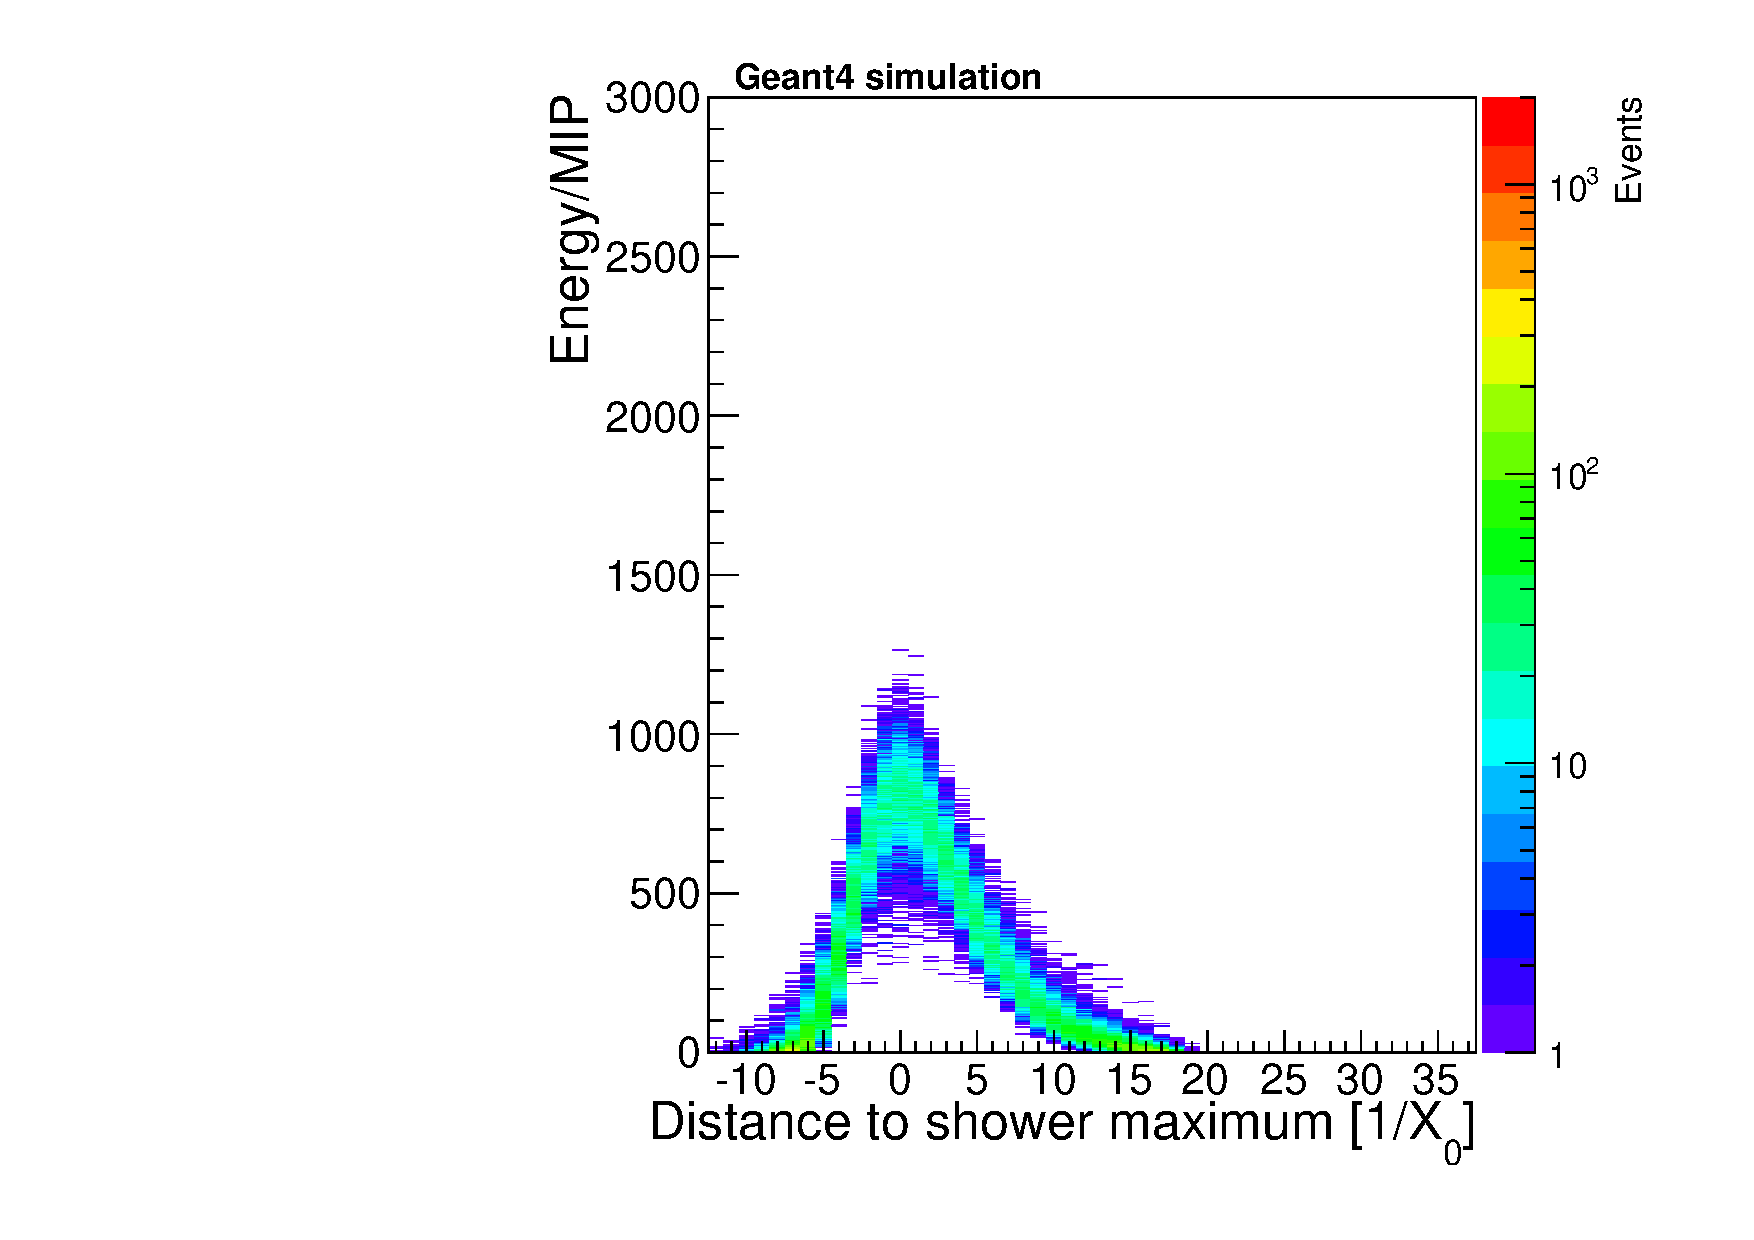
\includegraphics[width=0.23\textwidth]{figures/version_3e_75_showerprof}
    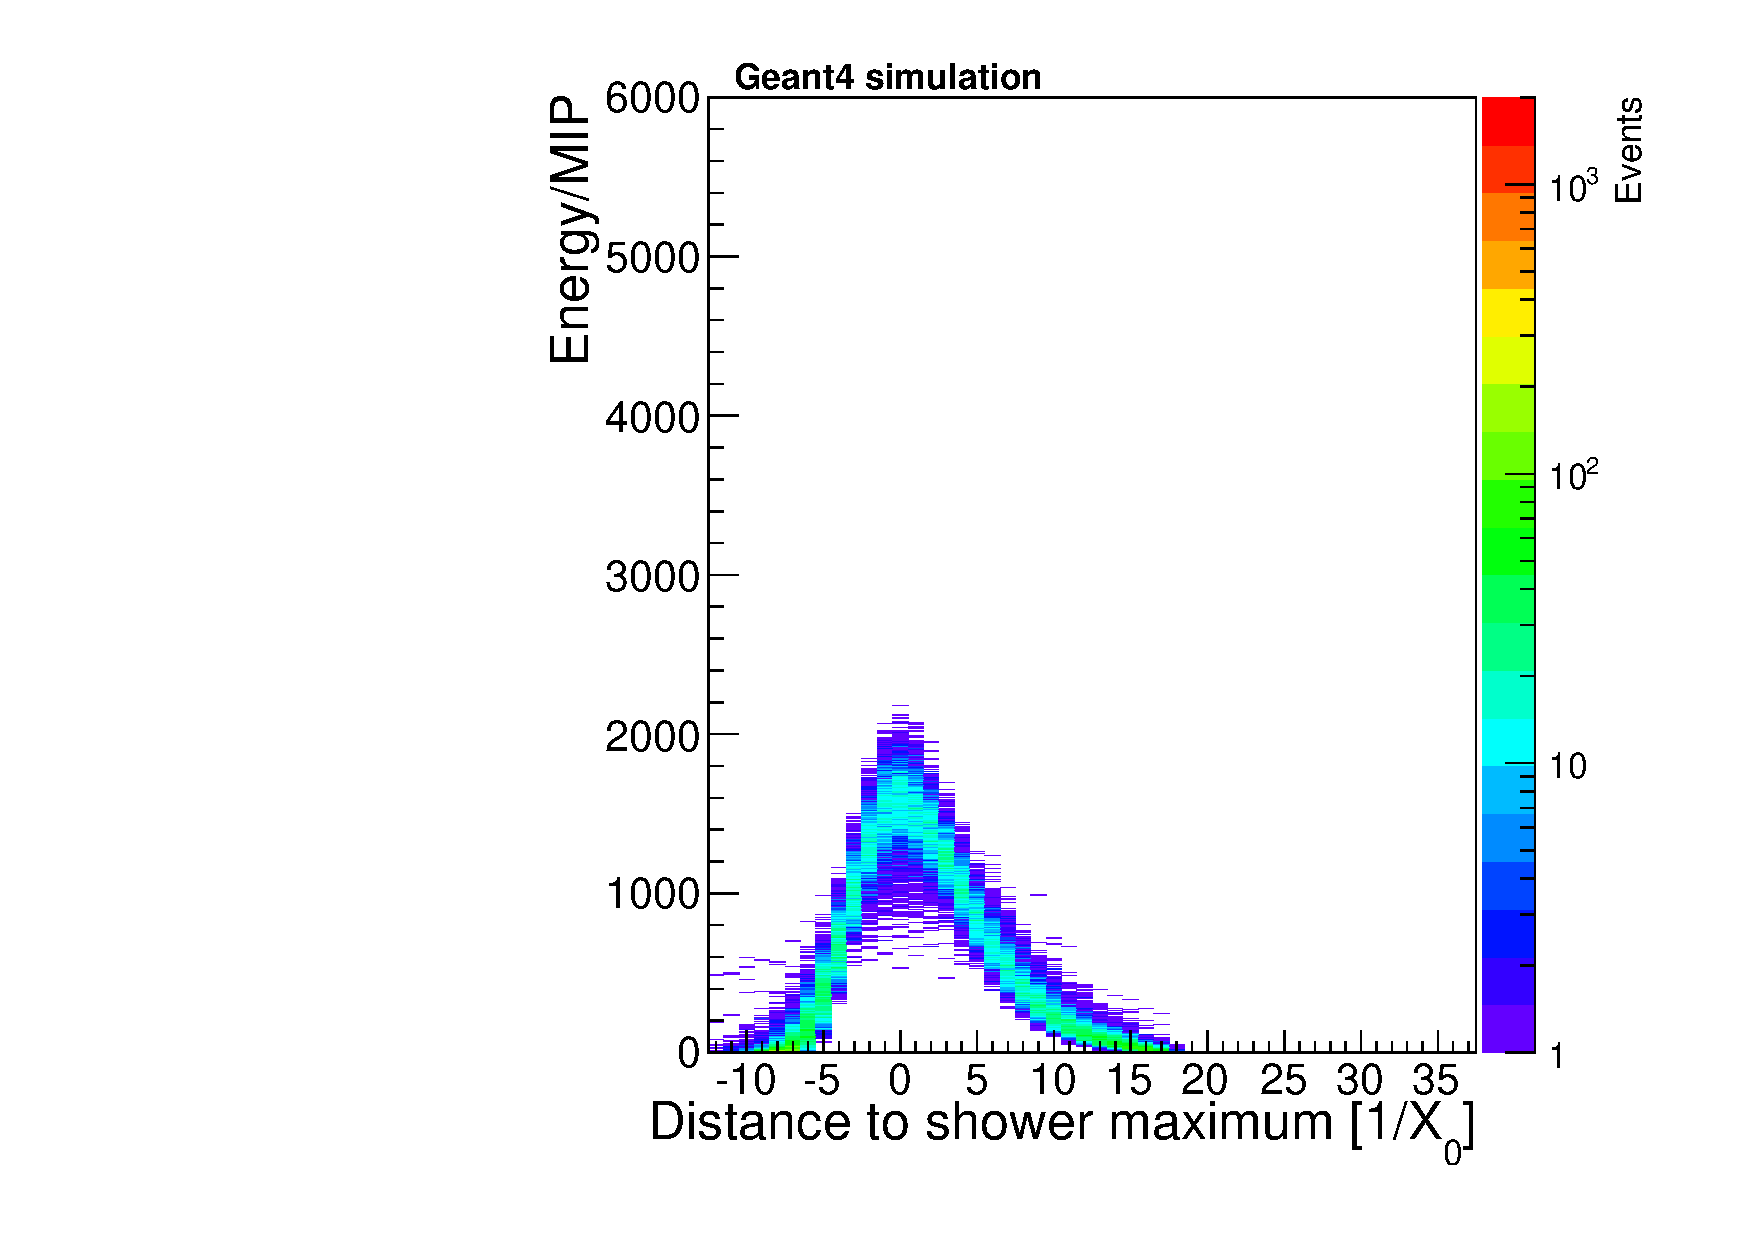
\includegraphics[width=0.23\textwidth]{figures/version_3e_150_showerprof}
    \caption{ Energy distributions versus the distance in \Xnot to the
      shower maximum for different electron energies. From {\em left}
      to {\em right} the incident electron energies are: 10\GeV,
      25\GeV, 75\GeV and 150\GeV.
   }
    \label{fig:longenergydep}
  \end{center}
\end{figure}

Figure~\ref{fig:longprofiles} summarizes the average energy profile
(and energy fluctuation) of the showers for different incident
energies.
The plot on the {\em left} is shown as function of the transversed
thickness transversed in the detector.
It can be observed that for incident energies below 5\GeV the shower
maximum will occur in average in the first section of the detector.
For energies up to 500\GeV the shower maximum will be contained in the
second section of the detector.
As explained above, the fitted longitudinal shower profile to each
event can be used as the estimator of the shower maximum. This
estimator can be used to re-map the energy deposits as function of the
distance to the shower maximum yielding the so-called centered shower
profile shown at the {\em right} of the figure.
This result depicts the scaling property of the energy generated by
the electromagnetic showers in the sensitive Si volumes,
which yield the linear behaviour of the energy estimators used above.

\begin{figure}[h!]
  \begin{center}
   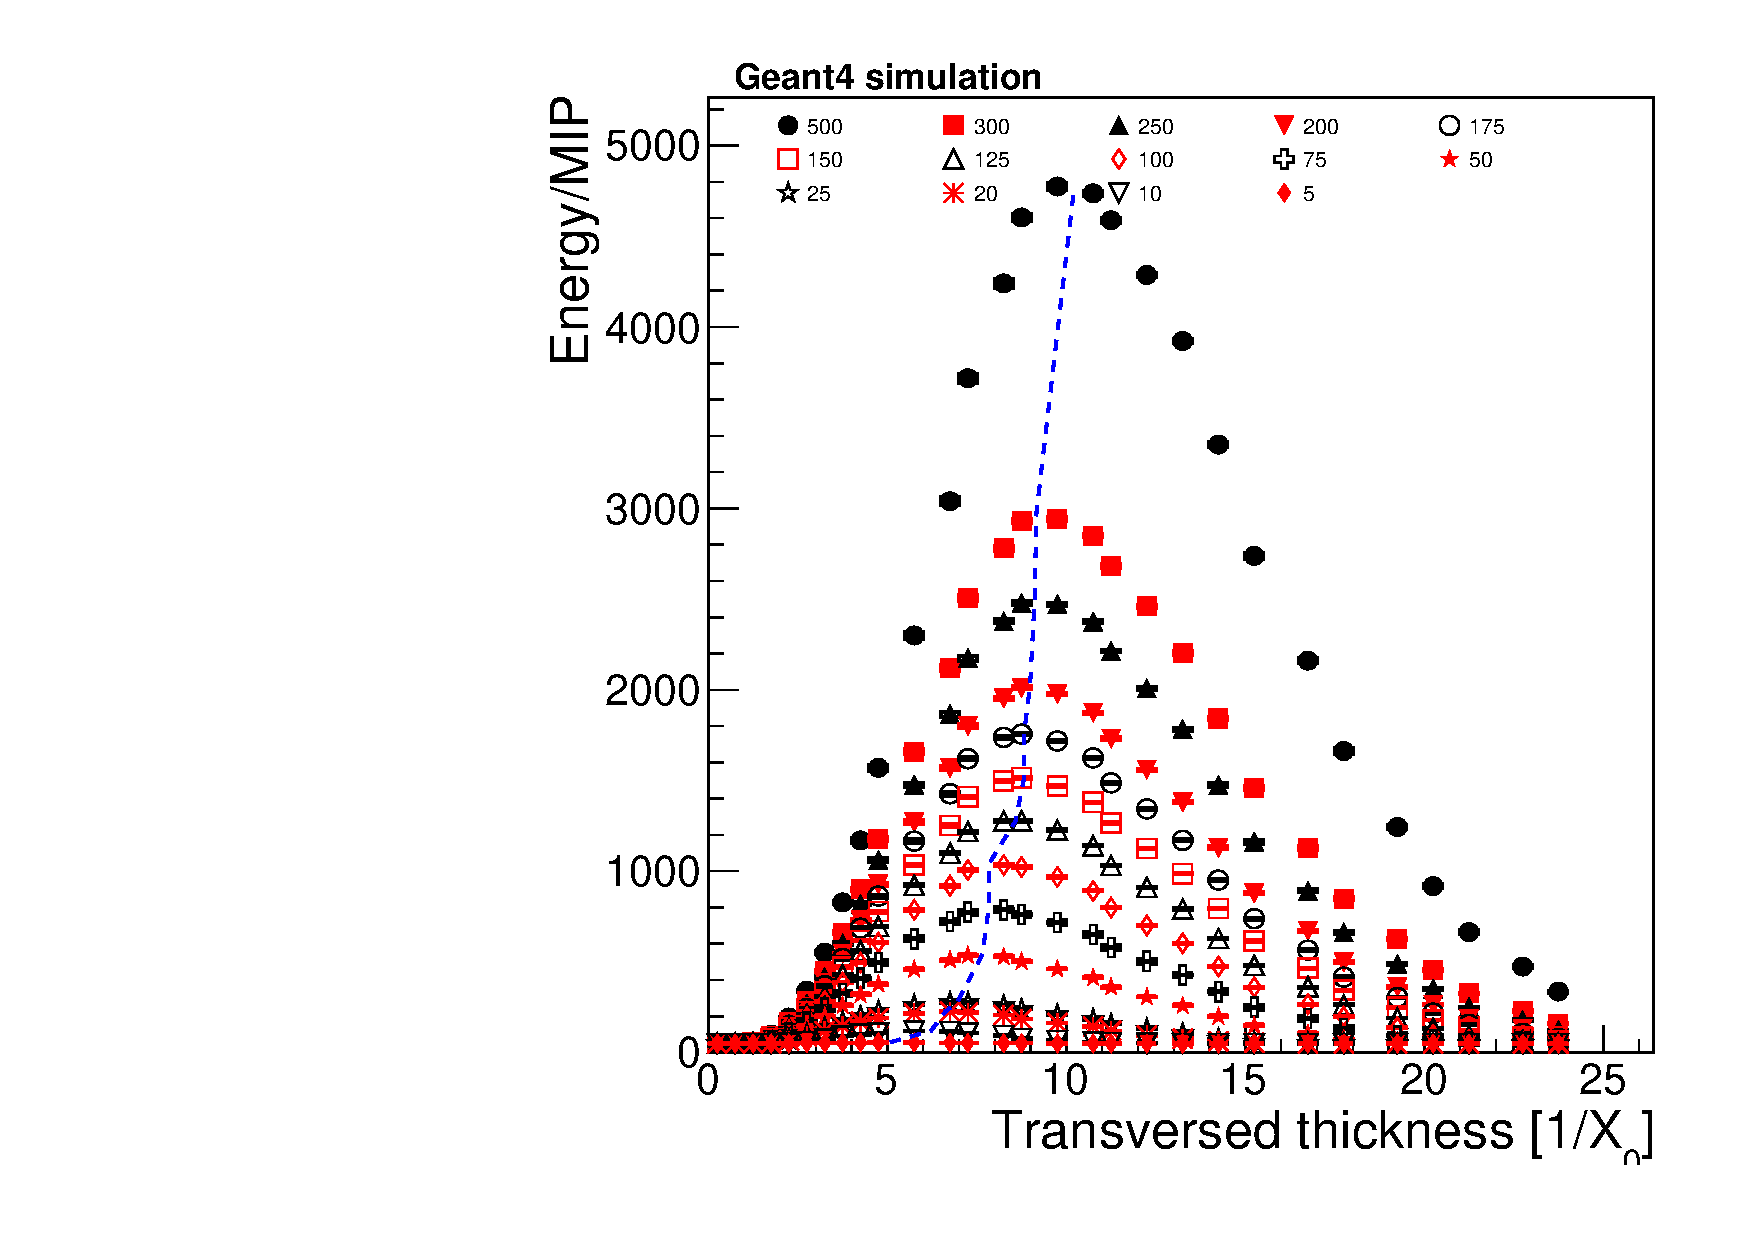
\includegraphics[width=0.49\textwidth]{figures/version_3_rawprof}
    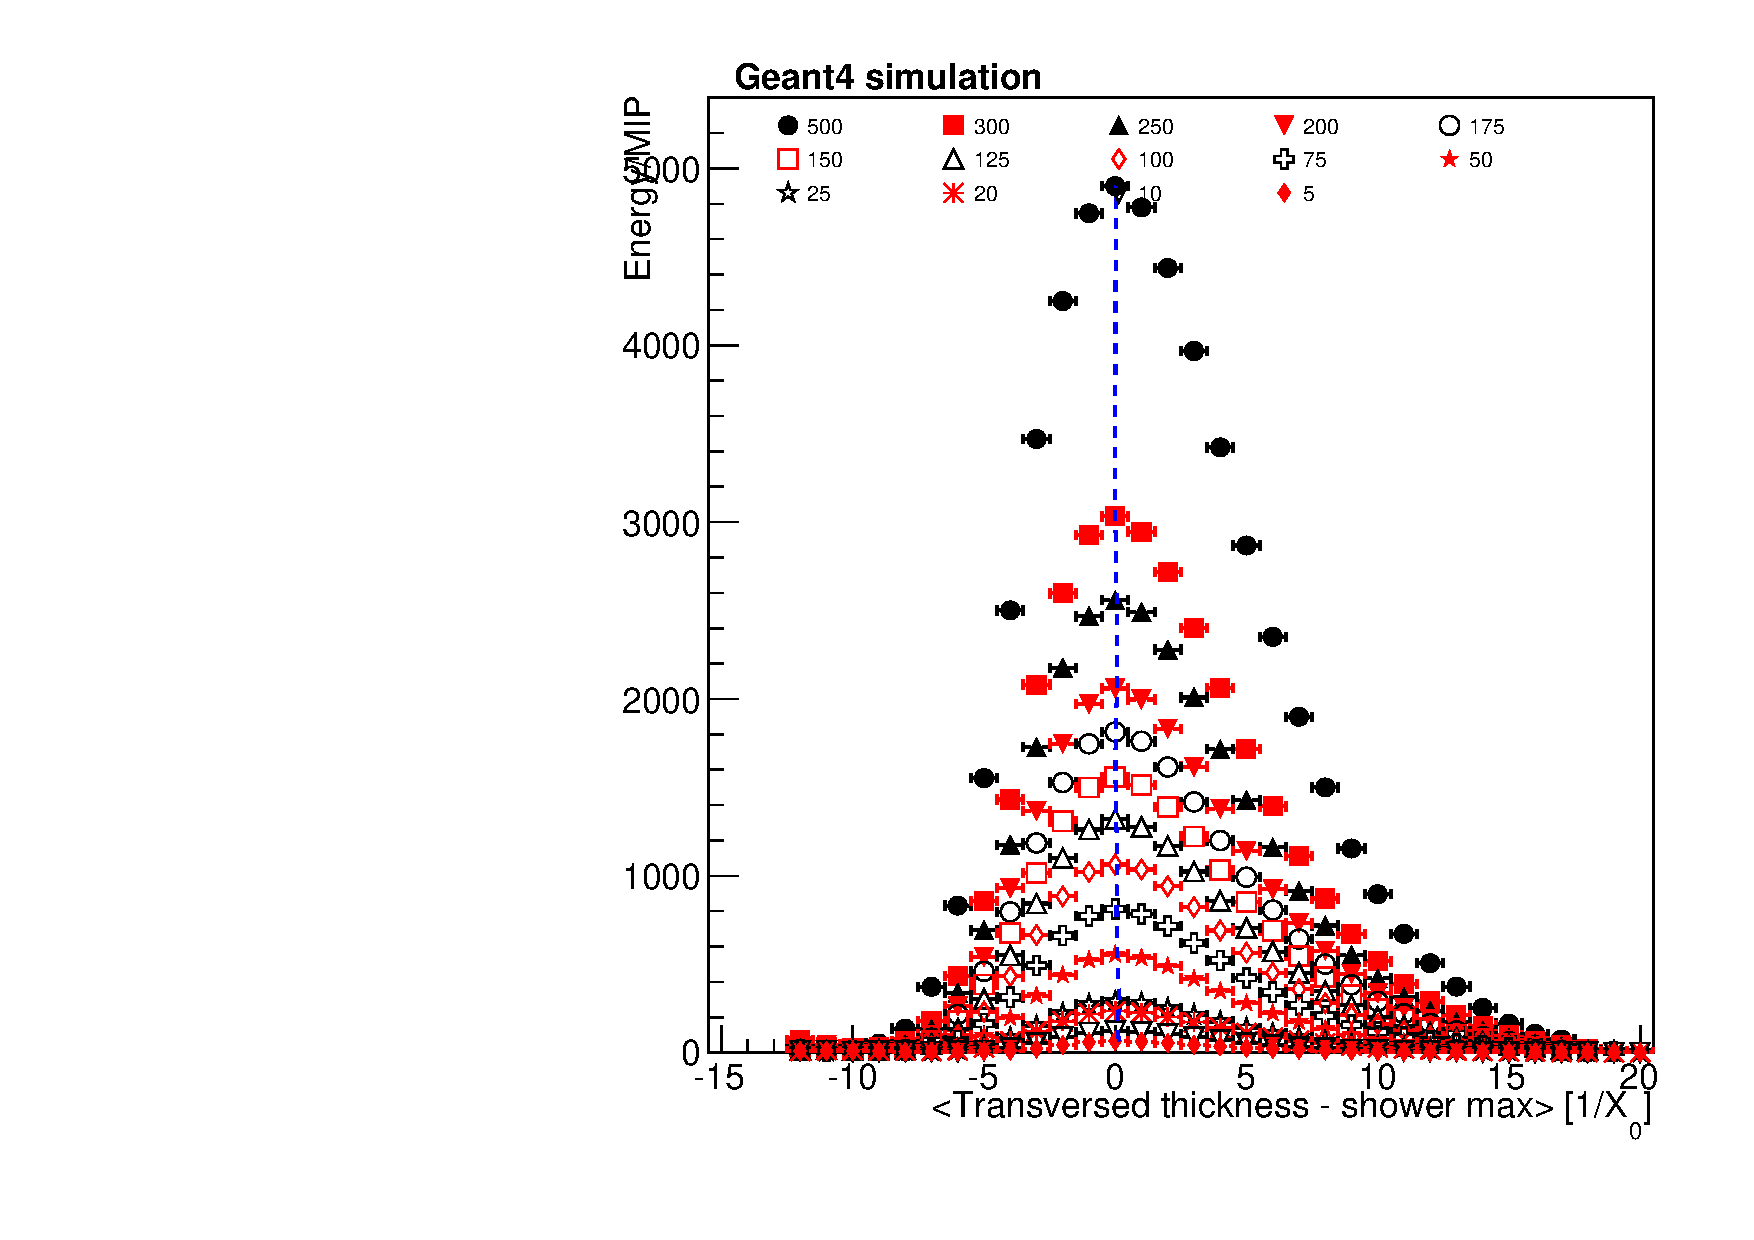
\includegraphics[width=0.49\textwidth]{figures/version_3_cenprof}
    \caption{{\em Left}: average energy deposited as function of the
      transversed thickness in the calorimeter. A blue curve connects
      the estimated shower maximum.
     {\em Right}: average energy deposited as function of the distance
     to the shower maximum estimated on an event-per-event basis.
    {\em Right}: average relative width of the energy deposits as
    function of the distance to the shower maximum estimated on an event-per-event basis.
   }
    \label{fig:longprofiles}
  \end{center}
\end{figure}

The centered shower profile can be furthermore used to profile the
average fluctuations. This is shown on Figure~\ref{fig:longprofilesunc}.
The core of the shower is, has expected, less prone to statistical
fluctuations with an intrinsic resolution of $<20\%$ for
$E>20\GeV$.
The initial stage is prone to the largest fluctuations and the fine
sampling at these earlier stages may therefore provide additional handle on the energy
resolution. This will be discussed later in Section~\ref{sec:optim}.
The last part of the shower, as it will be shown in the next Section, is expected to
be dominated by the halo of the shower and, again, is prone to larger
statistical fluctuations with respect to the central region.


\begin{figure}[h!]
  \begin{center}
    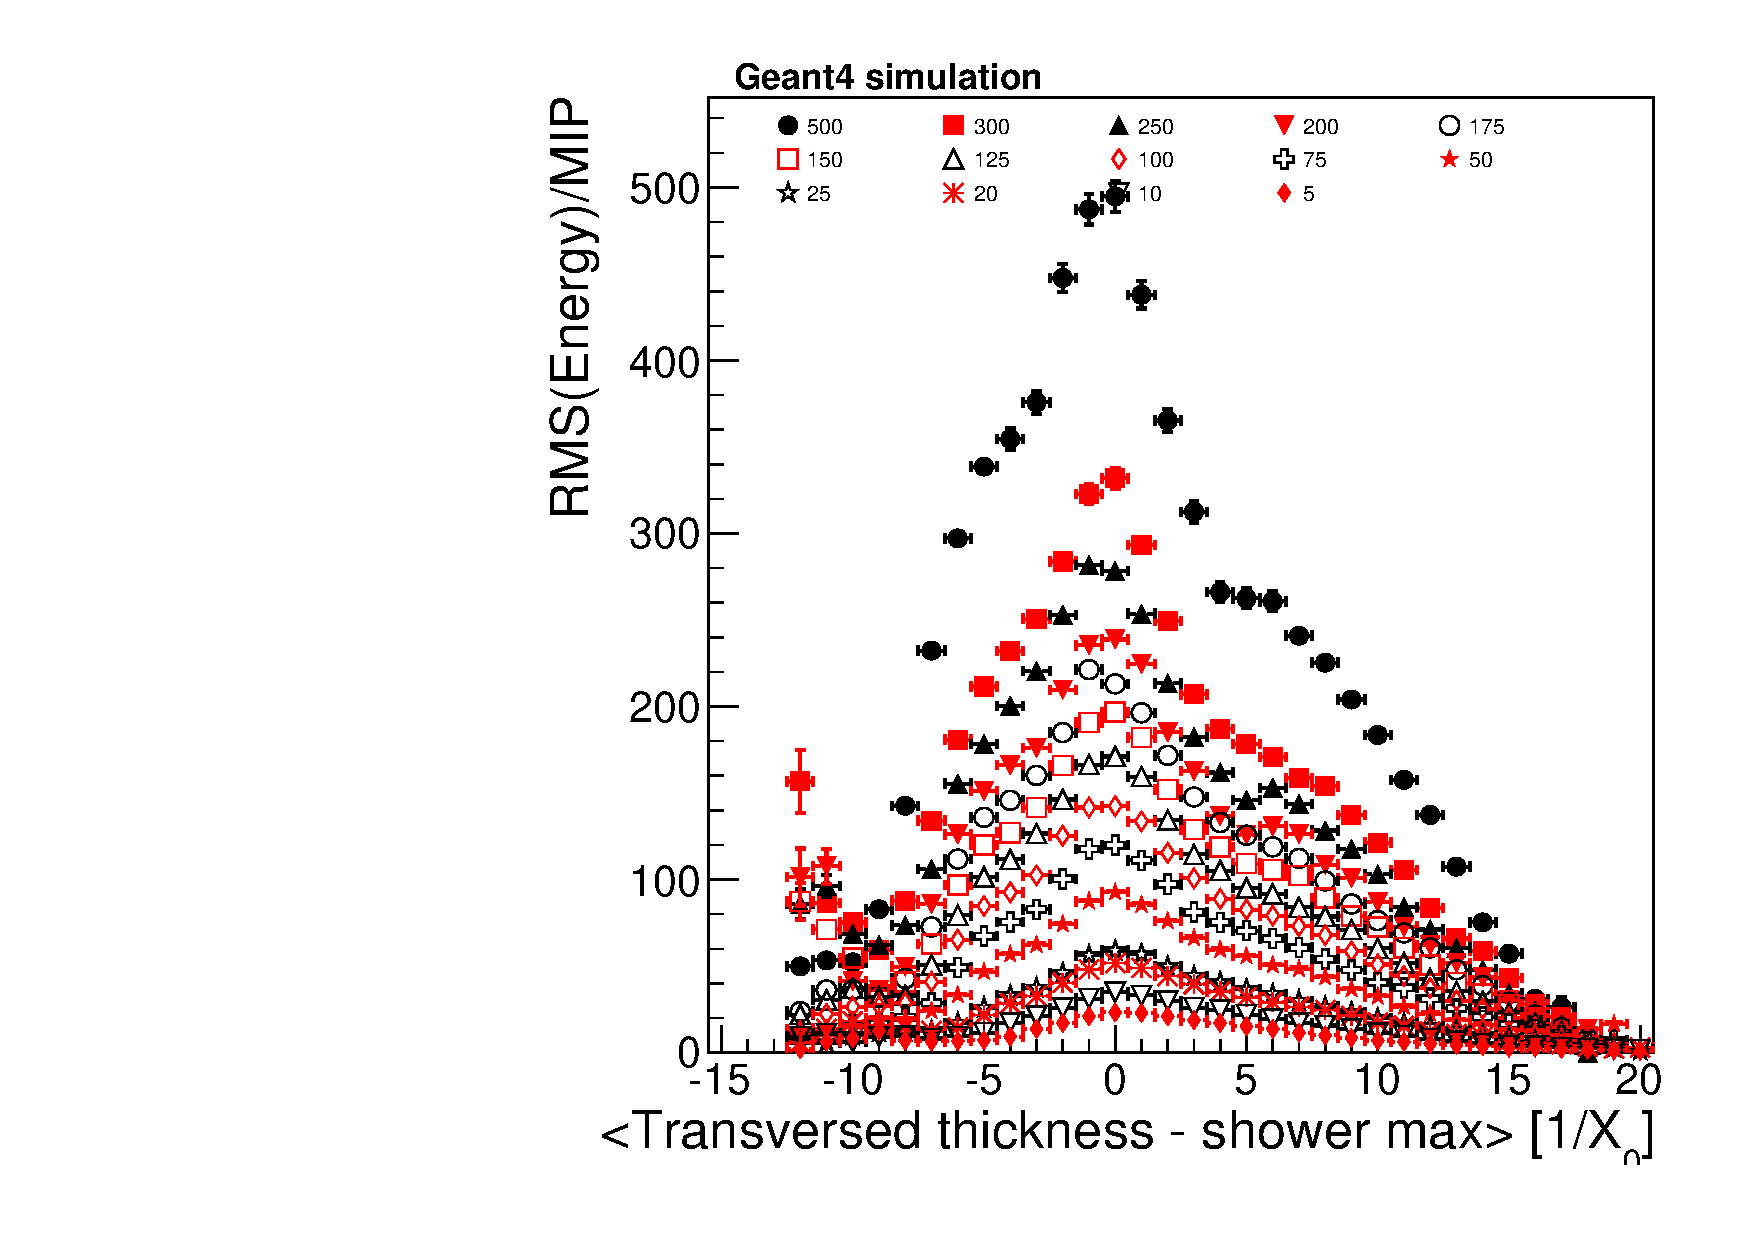
\includegraphics[width=0.49\textwidth]{figures/version_3_cenunc}
    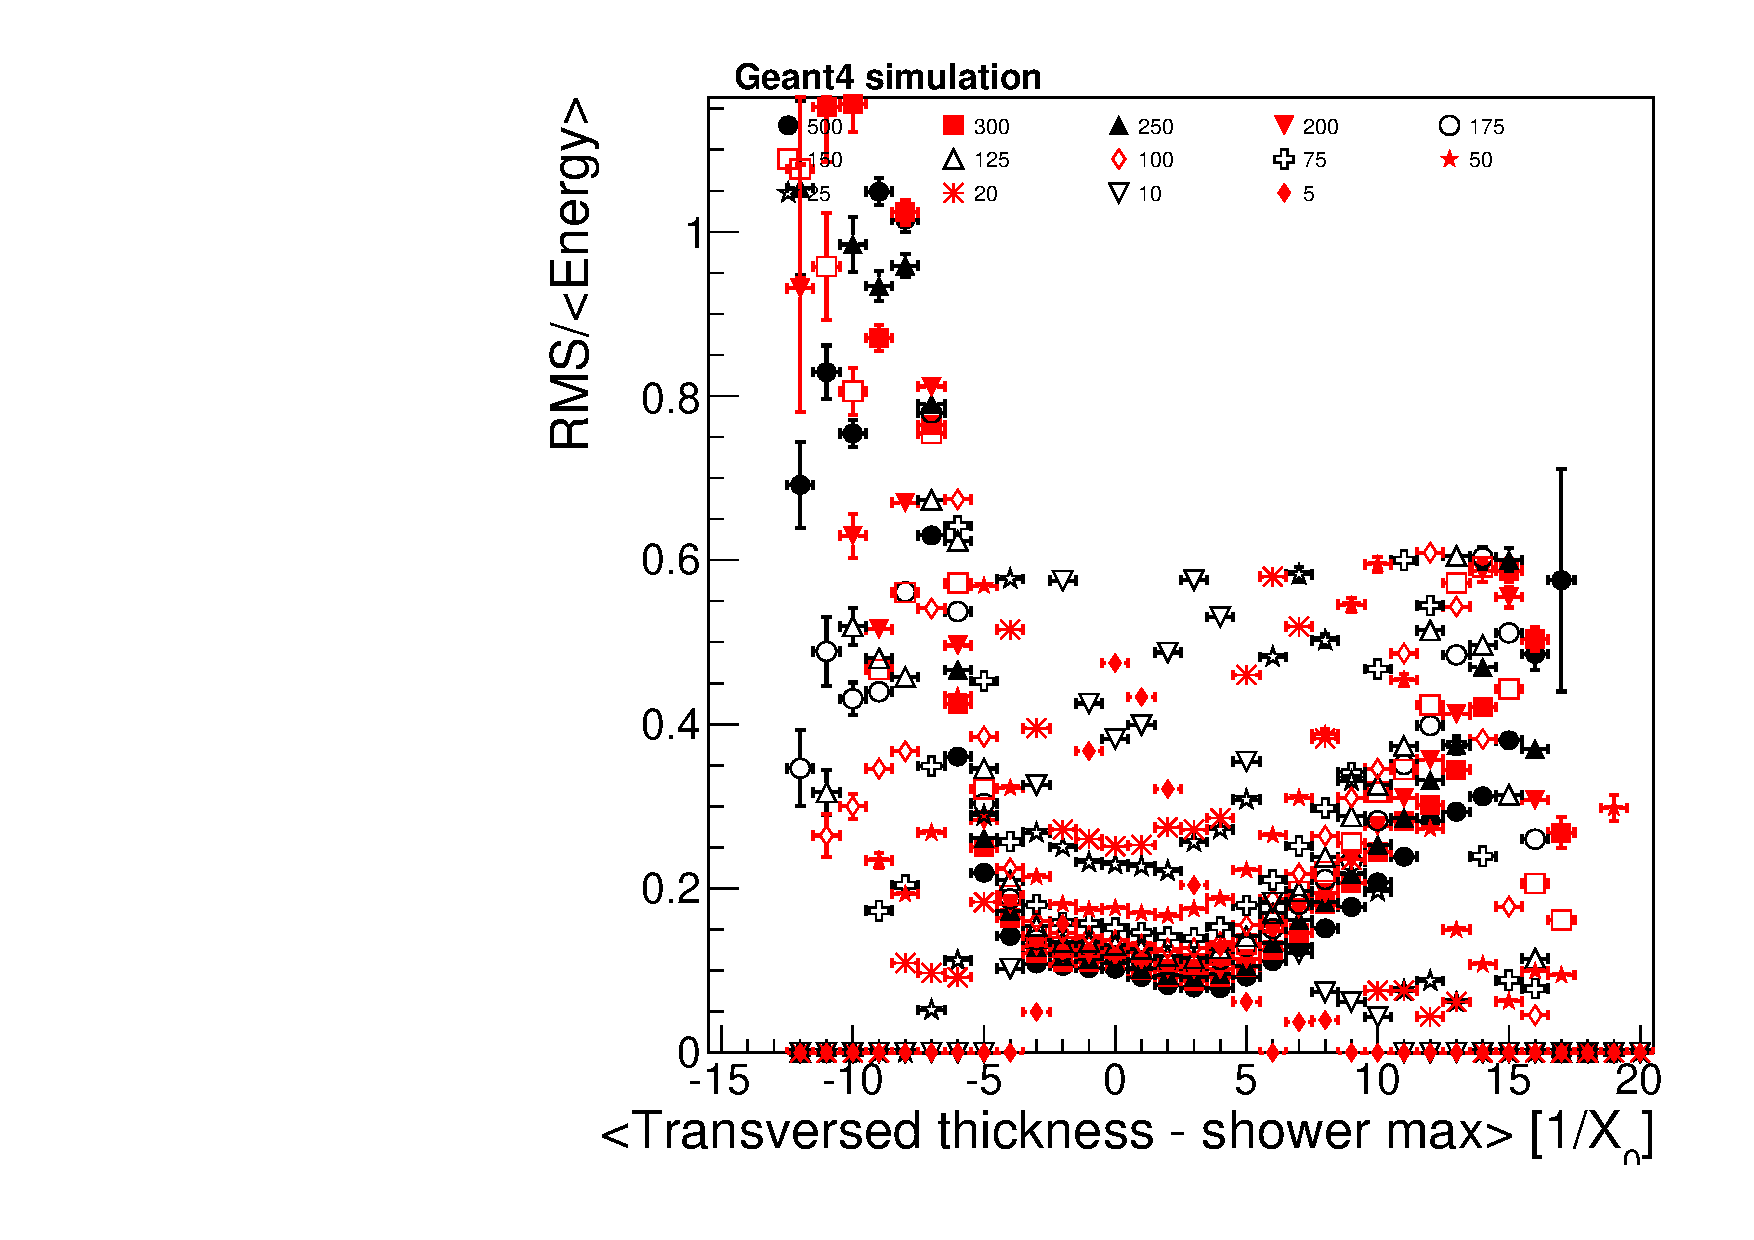
\includegraphics[width=0.49\textwidth]{figures/version_3_crelunc}
    \caption{{\em Left}: average width of the energy deposits.
    {\em Right}: average relative width of the energy deposits. Both
    quantities are represented as
    function of the distance to the shower maximum estimated on an event-per-event basis.
   }
    \label{fig:longprofilesunc}
  \end{center}
\end{figure}


%%
%%
%%
\subsection{Transverse shower evolution and shower containment}
\label{subsec:transvevol}

The generic properties of the evolution of the electromagnetic showers
in the transverse plane can be studied by sampling uniformly each Si
layer with a fine $2.5\times2.5\mm^2$ grid and counting the energy
deposits in each cell. The raw energy counted without up-weighting it based on
the per-sector weighting scheme described in the previous scheme.
Figures~\ref{fig:showertrans} show the evolution of two showers in the
transverse plane for incoming energies of 50\GeV and 150\GeV.
Using the radial distance $\rho=\sqrt{x^2+y^2}$ with respect to the
simulated electron beamline we can furthermore use these profiles to
obtain the average energy deposited as function of the distance to the
shower center as well as shower energy fraction contained within a
given distance to the shower center.
These results are illustrated, for the same incident energies, in
Figures~\ref{fig:showertransavgen} and~\ref{fig:showertransavgenfrac}.
One can observe that the showers are narrow being 90\% of the energy
contained within 20\cm up to the shower maximum. After that the
profile of the energy is less centered (halo-like) and the energy is
spread over the plane. The 90\% radius tends to increase exponentially
after each layer.

\begin{figure}[h!]
  \begin{center}
    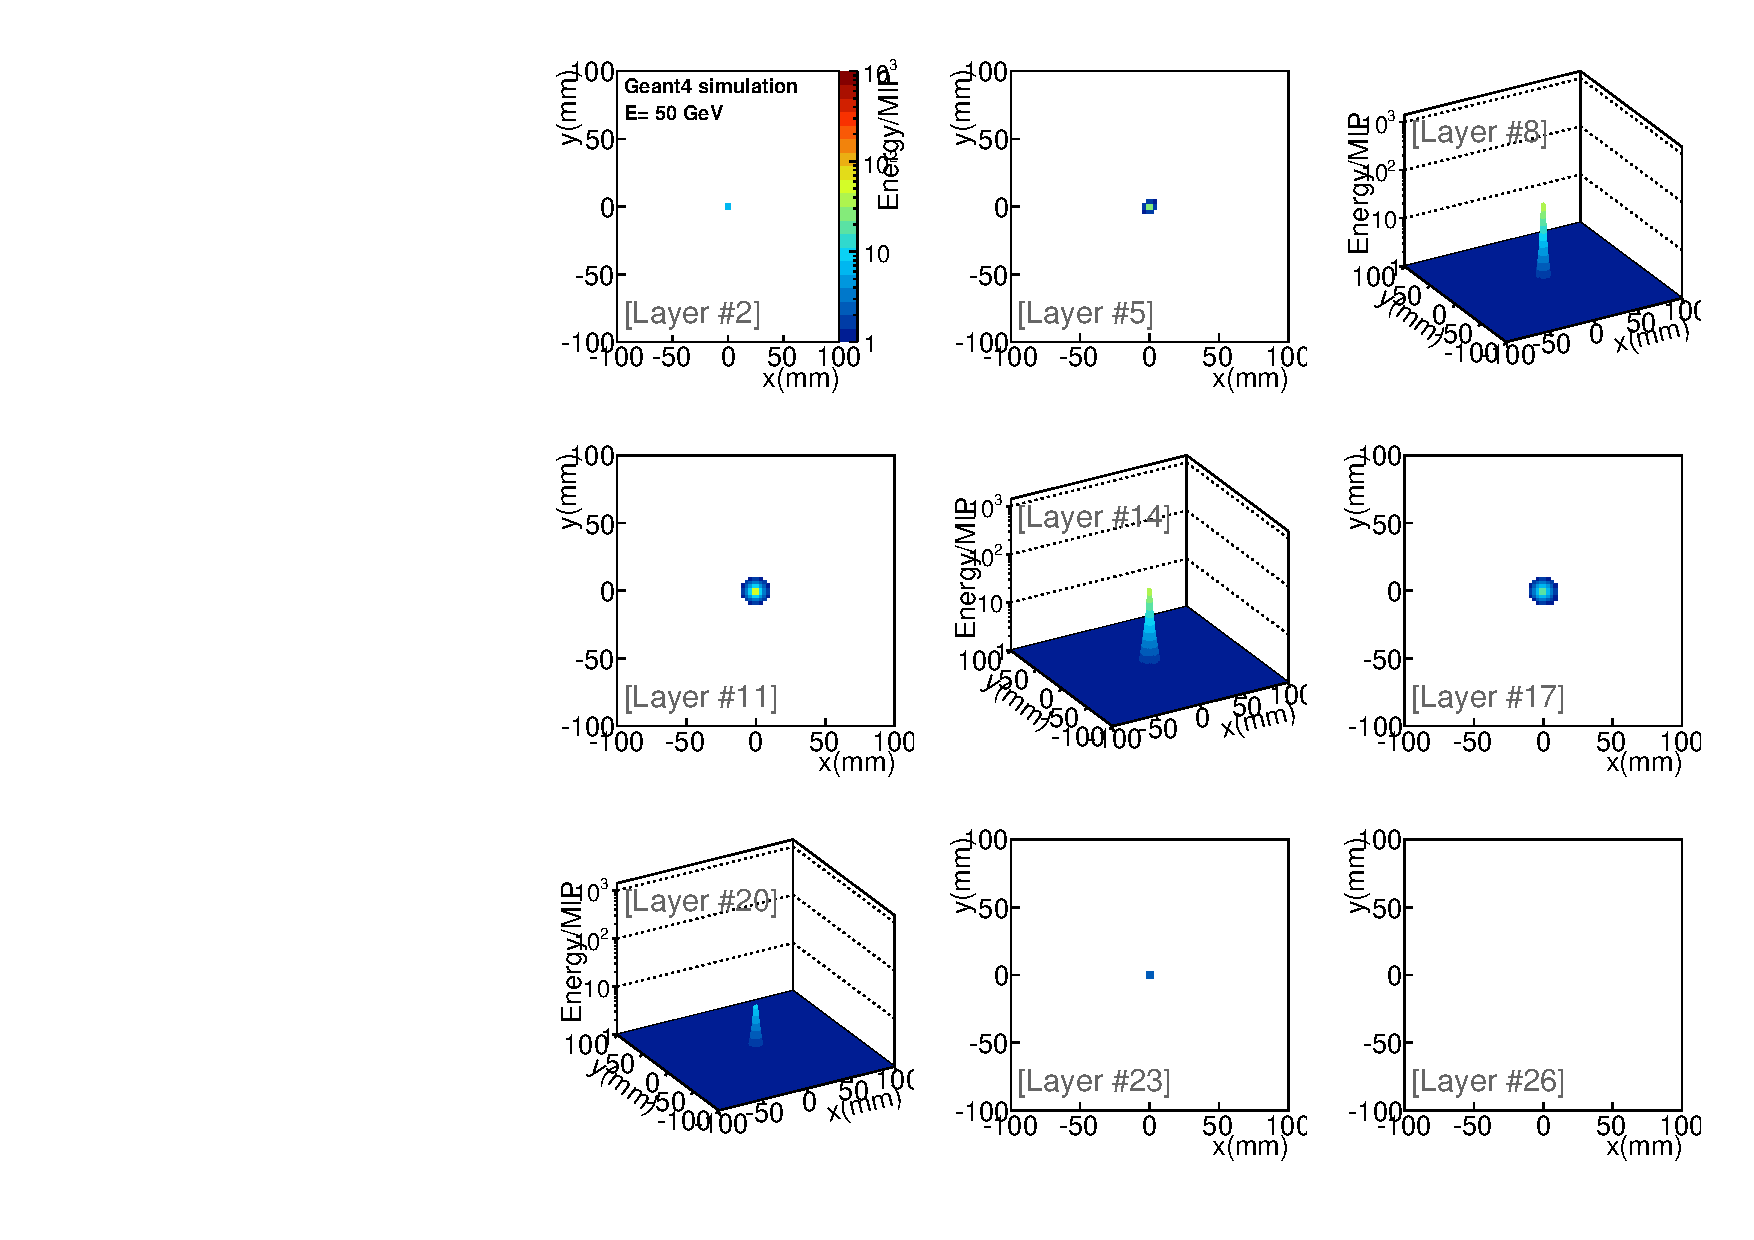
\includegraphics[width=0.7\textwidth]{figures/cxysensorenhitsvsrE50}
    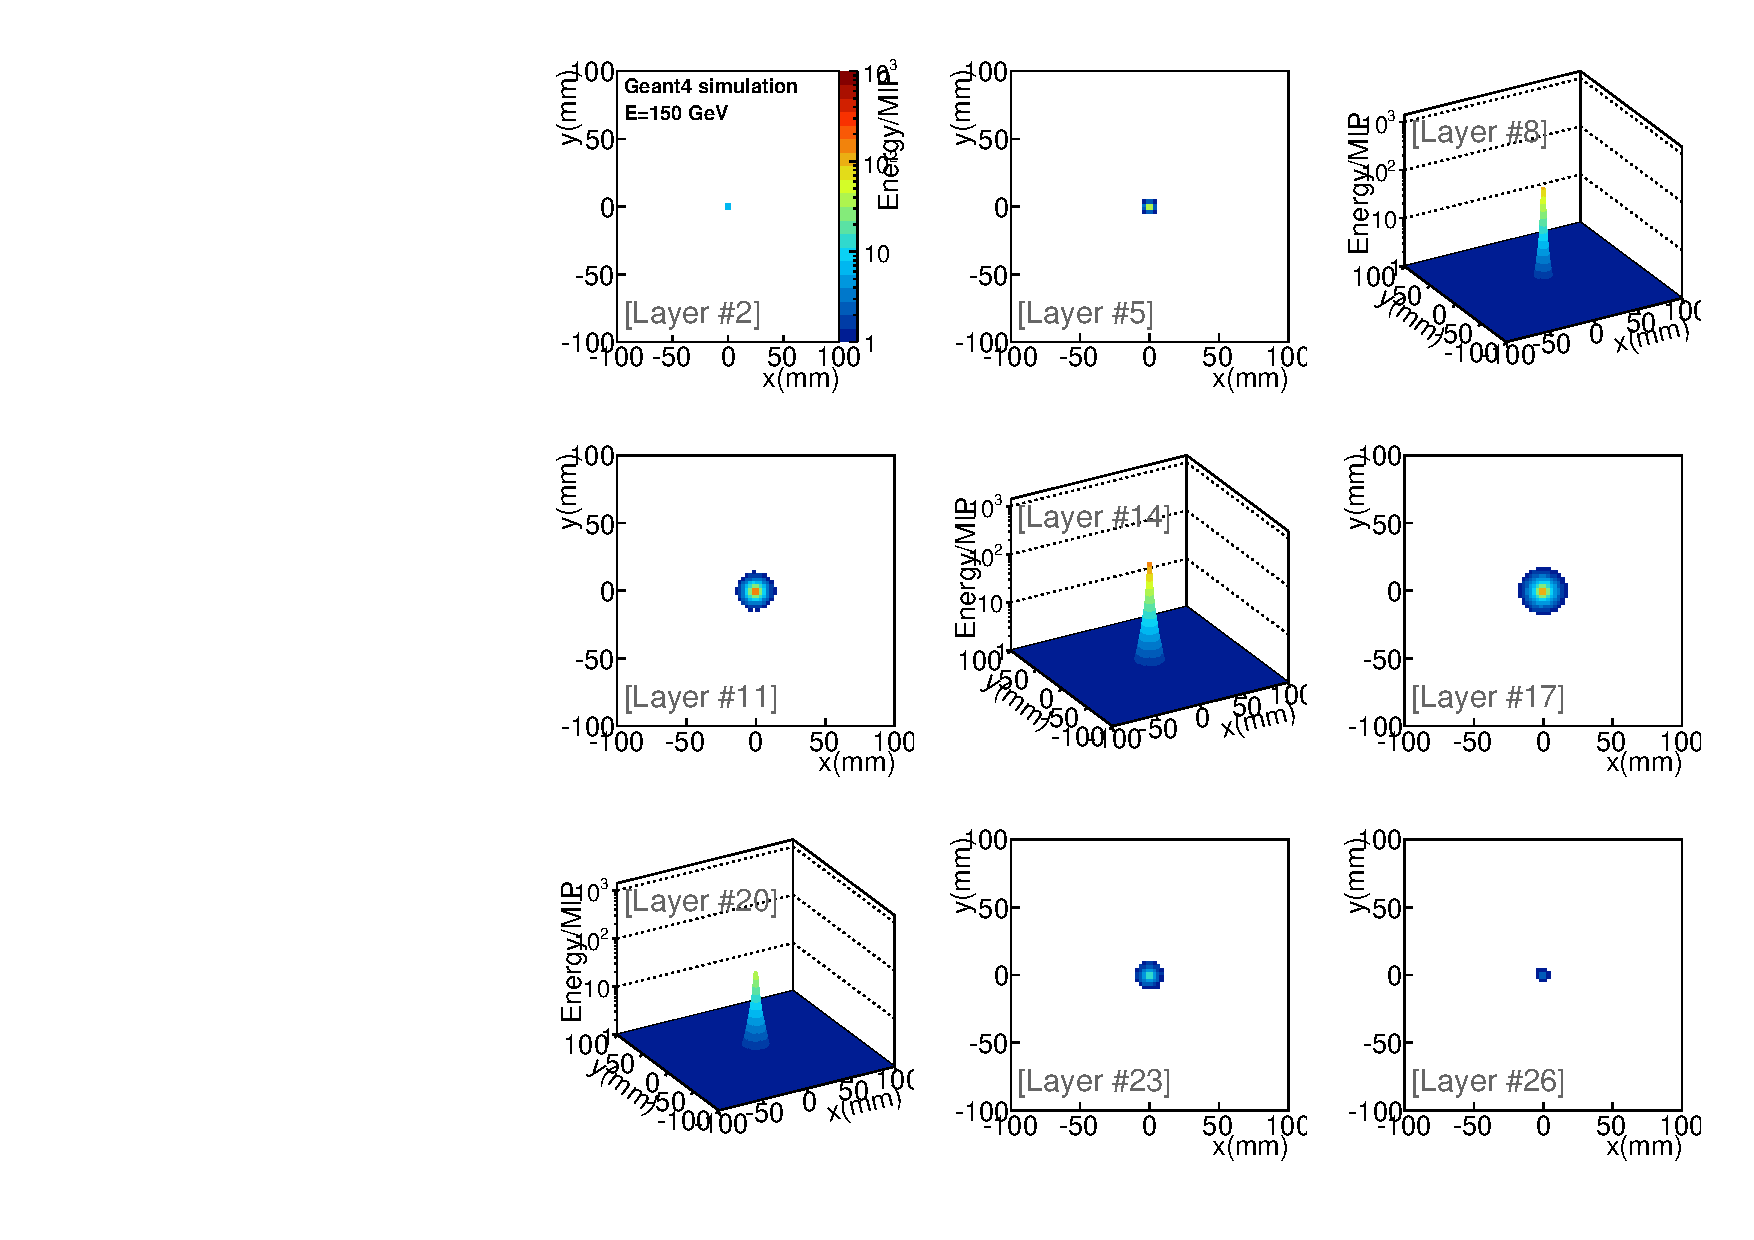
\includegraphics[width=0.7\textwidth]{figures/cxysensorenhitsvsrE150}
    \caption{Average evolution of electromagnetic showers in the transverse
      plane for selected Si layers. The per-sector weights are applied
      to the energy measured in MIP equivalents. Incoming electrons
      with E=50\GeV (150\GeV) are shown on {\em top} ({\em bottom}).
   }
    \label{fig:showertrans}
  \end{center}
\end{figure}

\begin{figure}[h!]
  \begin{center}
    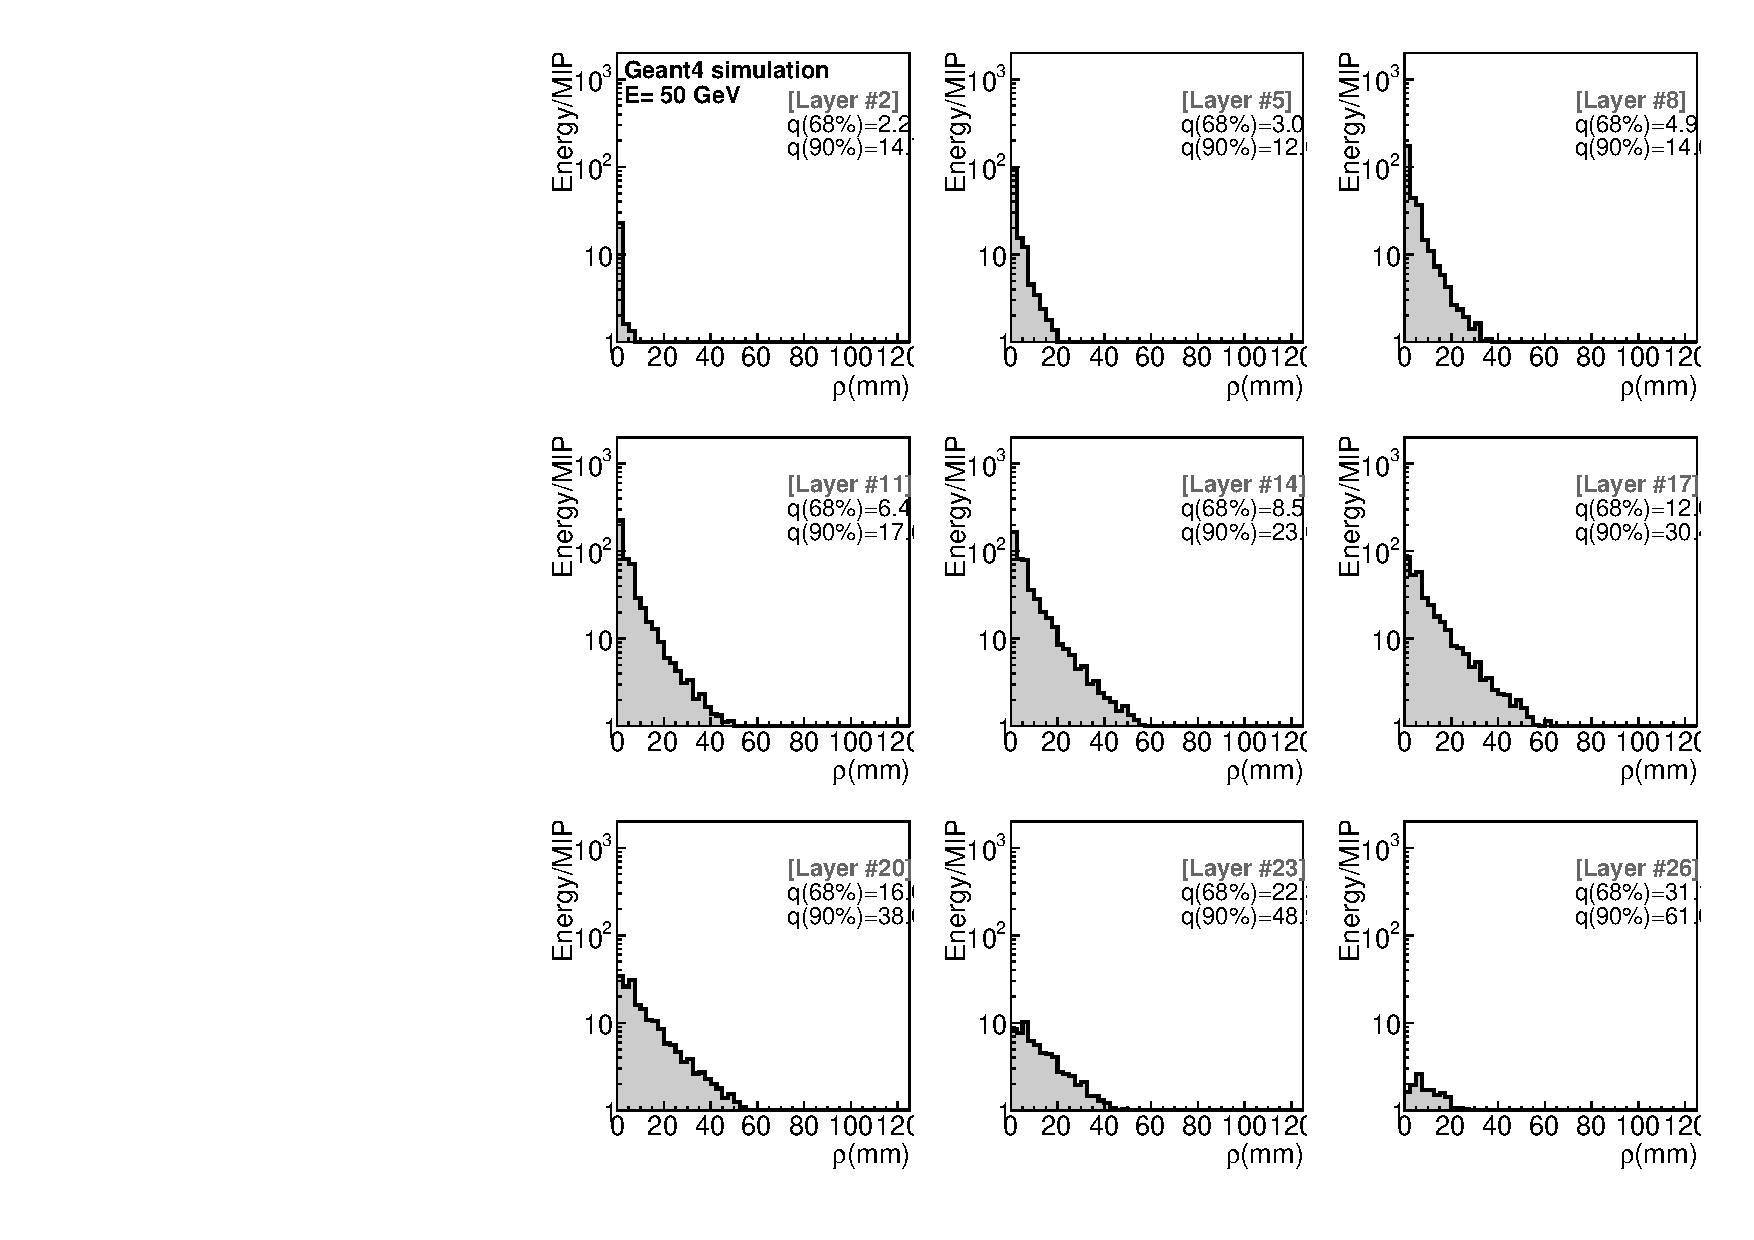
\includegraphics[width=0.7\textwidth]{figures/csensorenhitsvsrE50}
    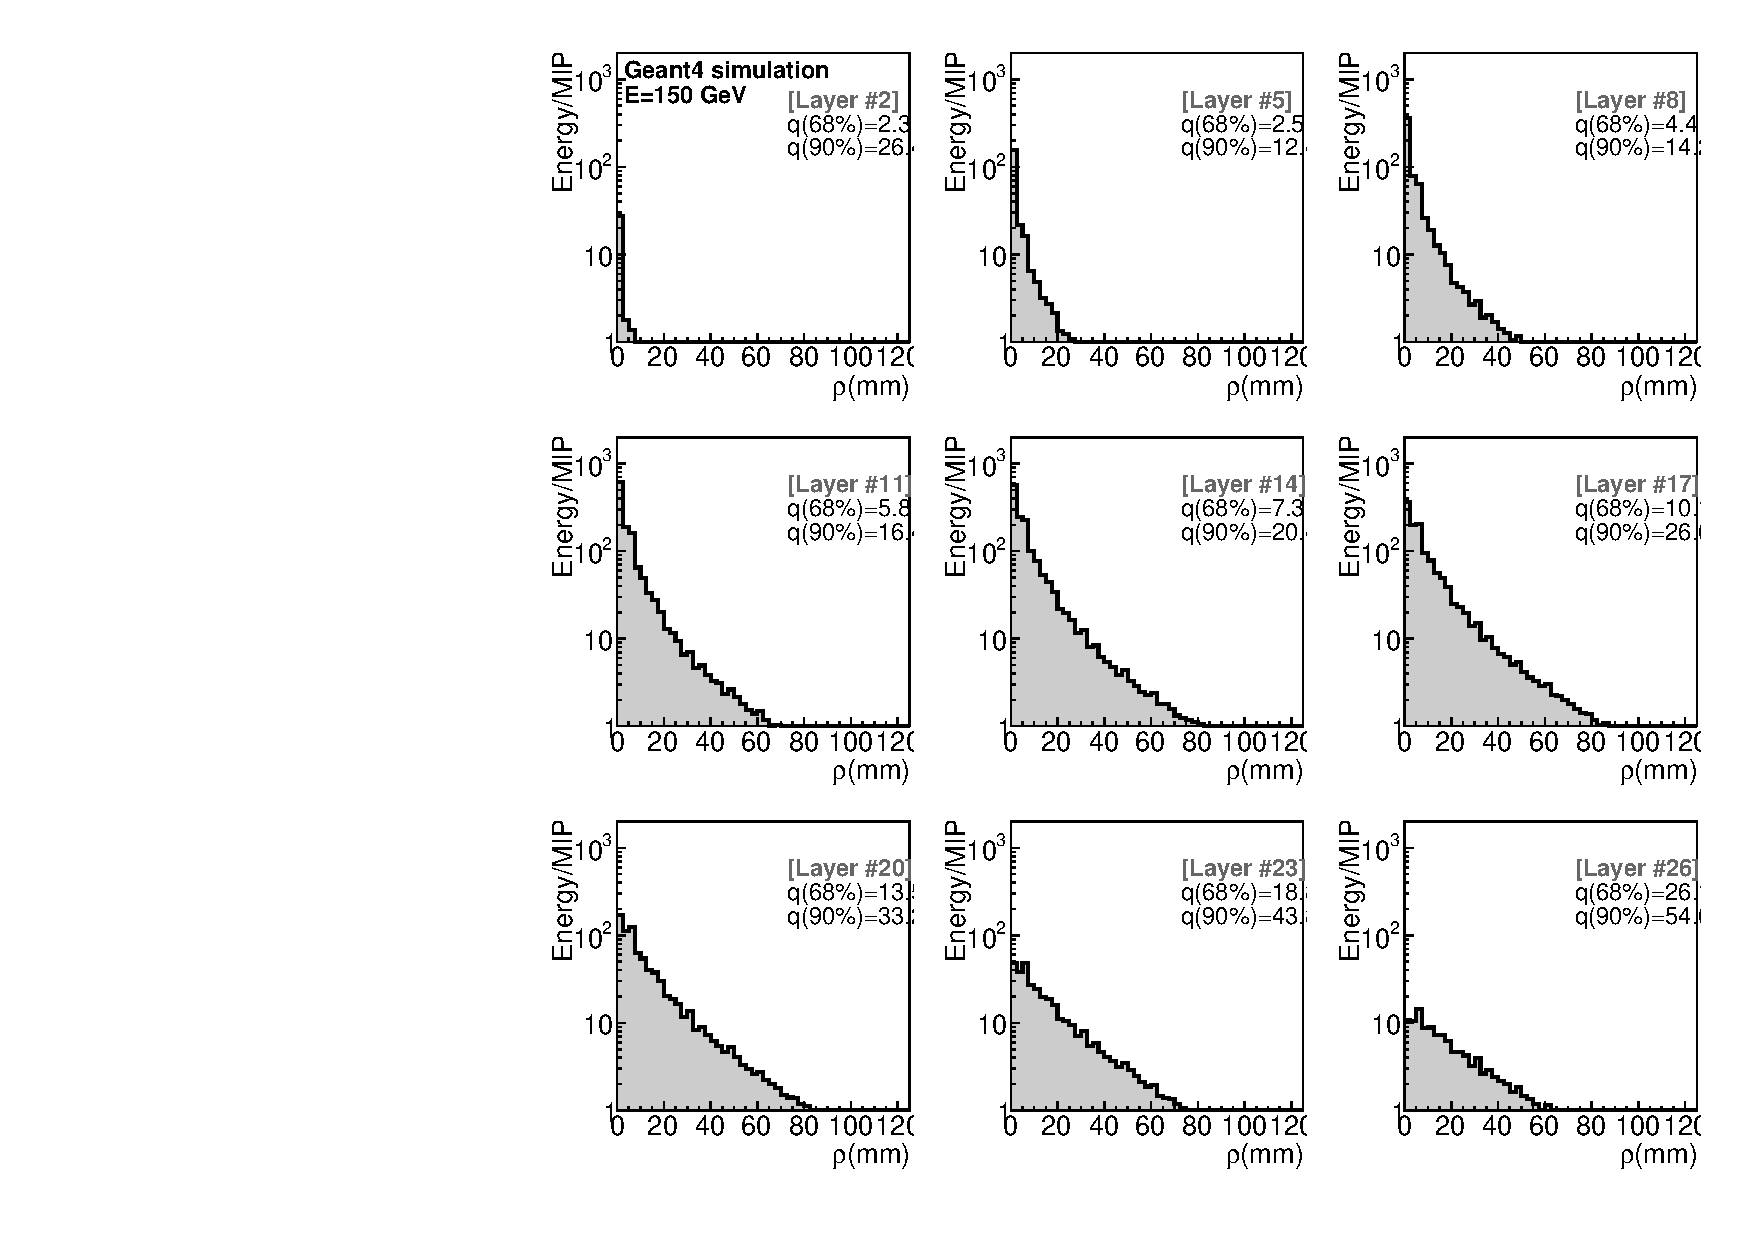
\includegraphics[width=0.7\textwidth]{figures/csensorenhitsvsrE150}
    \caption{Average energy deposited as function of the distance to
      the shower center.  Incoming electrons
      with E=50\GeV (150\GeV) are shown on {\em top} ({\em bottom}).
     In the captions, the distances corresponding to the 68\% and 90\%
    quantiles of the distributions are quoted.
   }
    \label{fig:showertransavgen}
  \end{center}
\end{figure}

\begin{figure}[h!]
  \begin{center}
    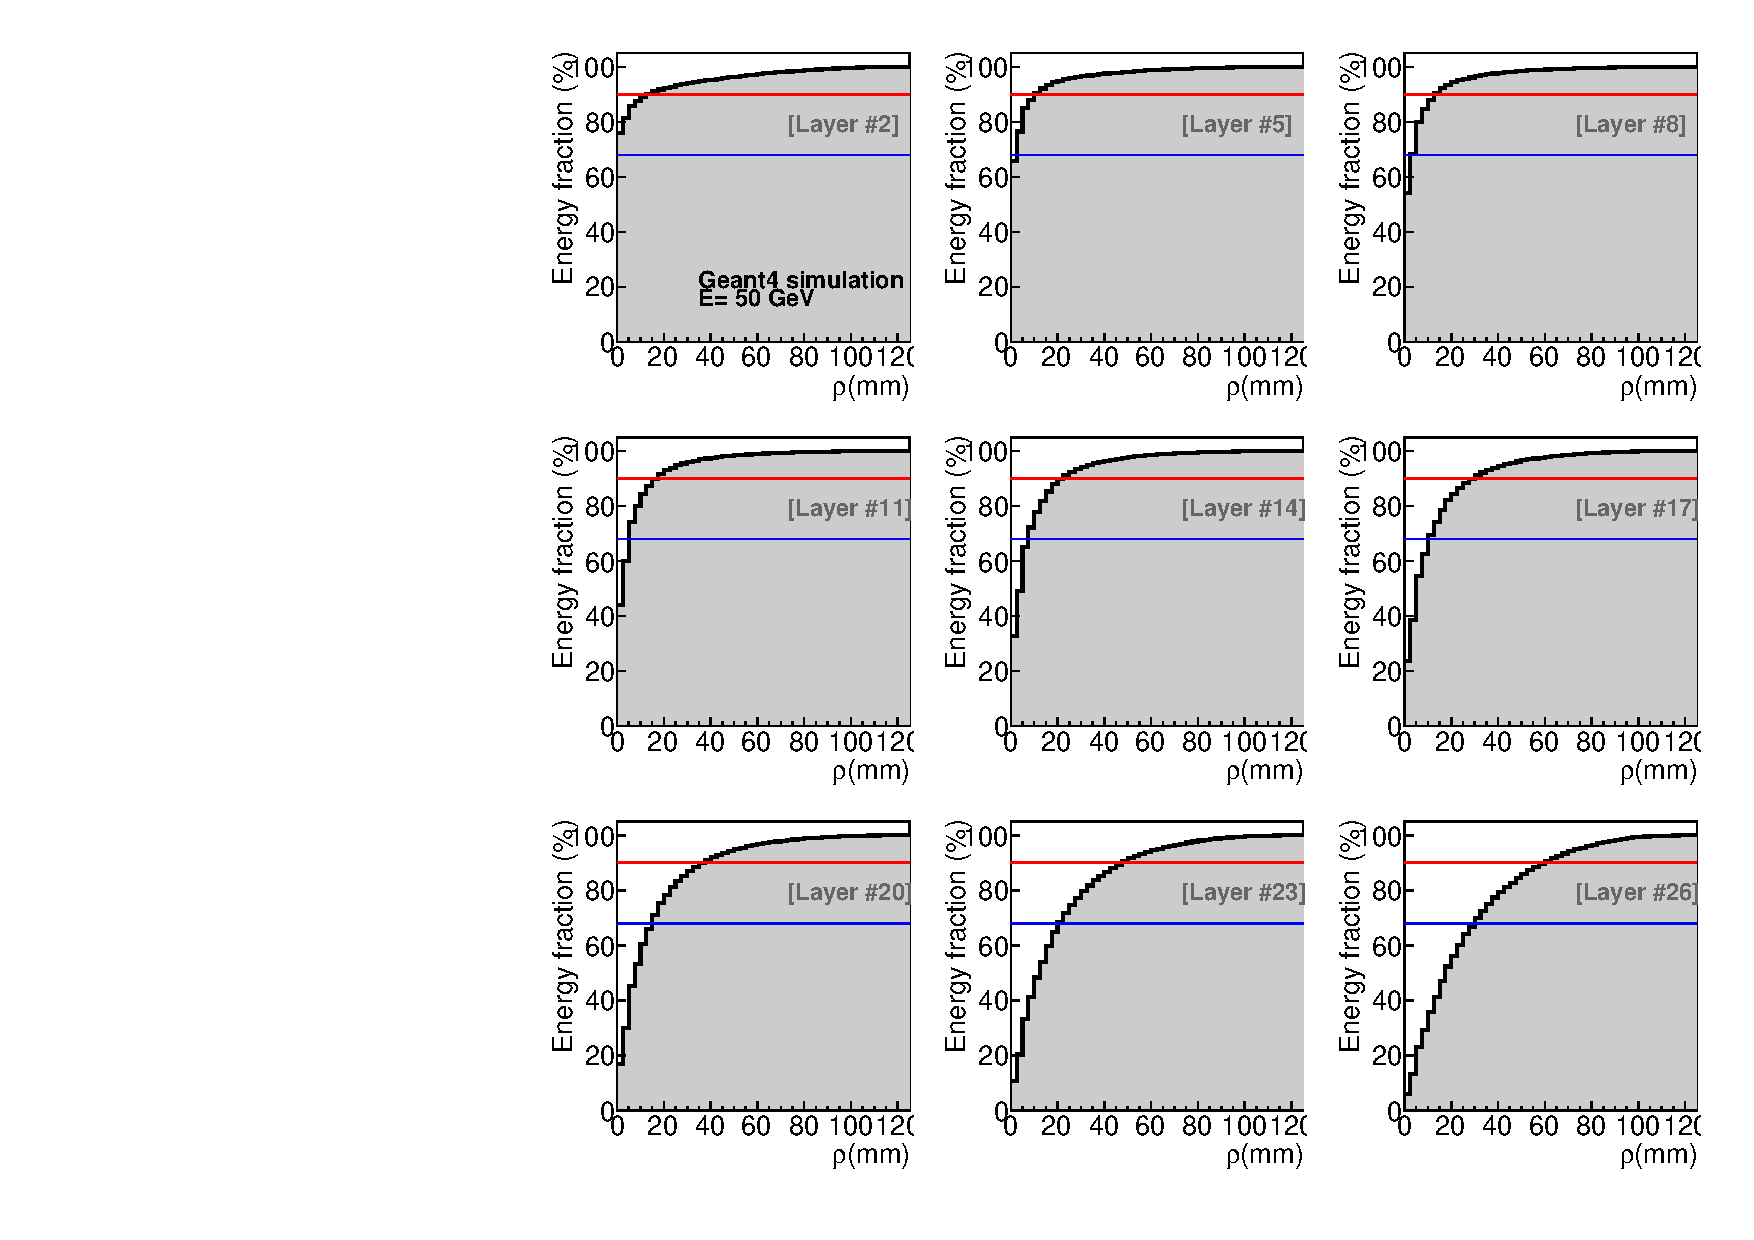
\includegraphics[width=0.7\textwidth]{figures/cfracsensorenhitsvsrE50}
    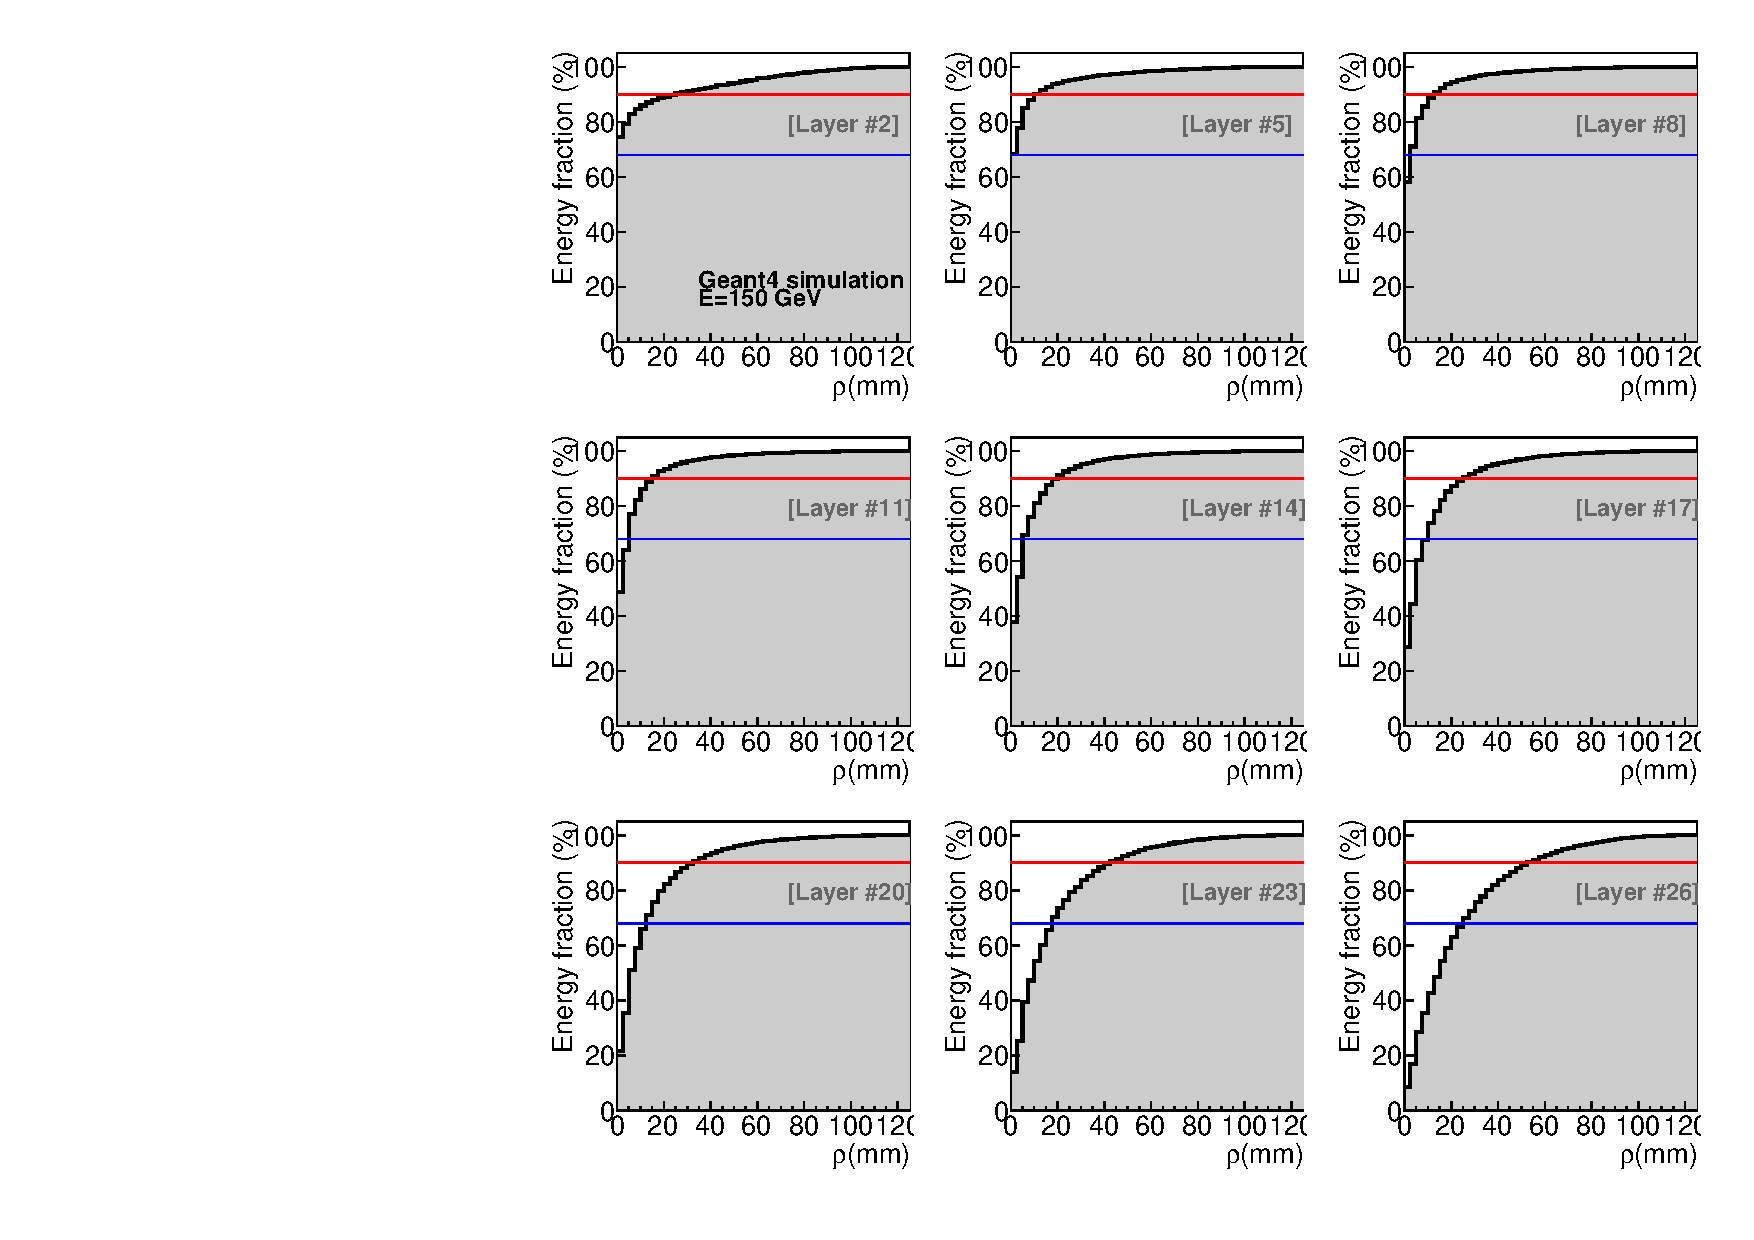
\includegraphics[width=0.7\textwidth]{figures/cfracsensorenhitsvsrE150}
    \caption{Average energy fraction contained within a given distance
      to the shower center. Incoming electrons
      with E=50\GeV (150\GeV) are shown on {\em top} ({\em bottom}).
      The blue and red lines mark the radius for which 68\% and 90\%
      of the energy are contained, correspondingly.
   }
    \label{fig:showertransavgenfrac}
  \end{center}
\end{figure}

Figure \ref{fig:showertranssummary} shows the evolution of the 68\%
and 90\% containment radius as function of the layer as well as the
dynamic energy range, \i.e. the average maximum energy deposited at
each layer and the average energy expected to be observed at the 90\%
containmnent radius.
The ratio of the two energies is expected to be approximately
similar for different incoming electron energies, indicating the
scaling properties of the electromagnetic shower.


\begin{figure}[h!]
  \begin{center}
    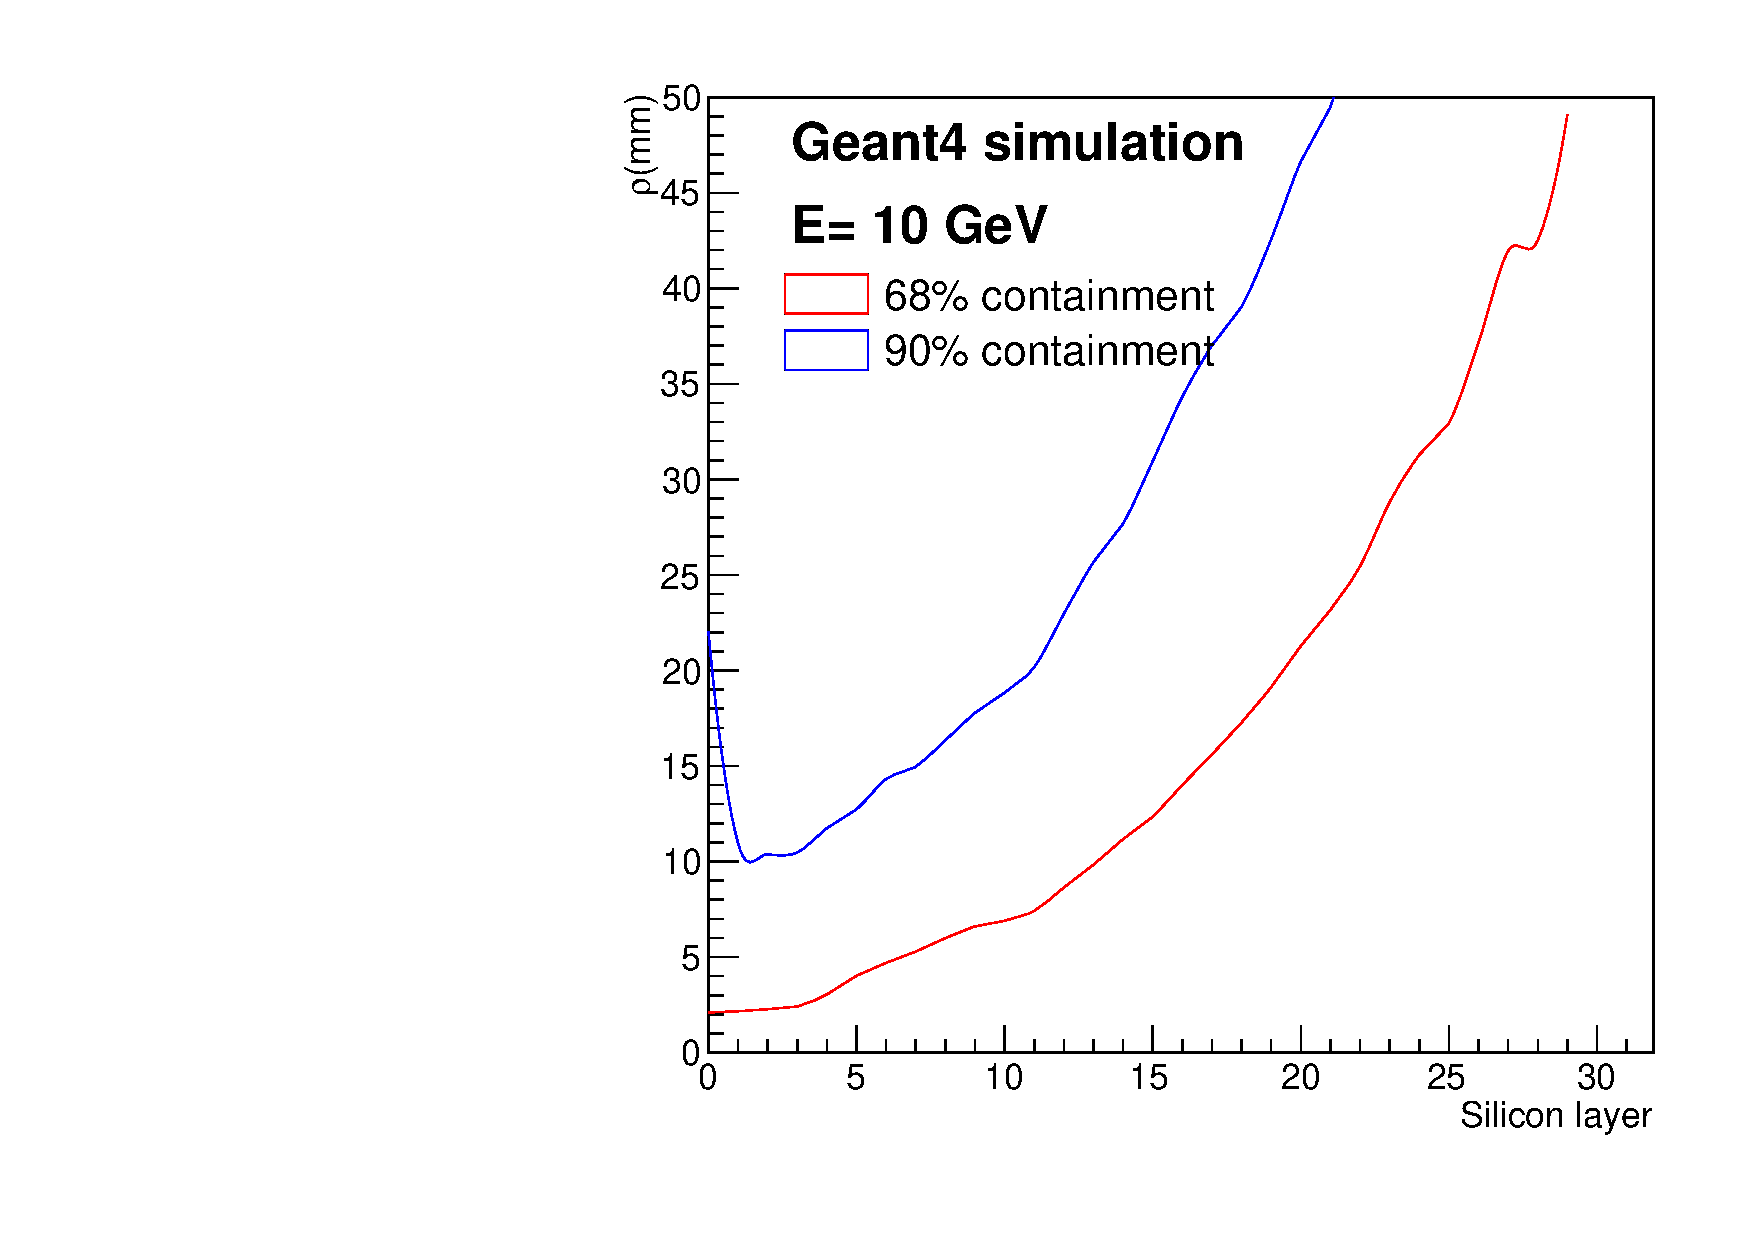
\includegraphics[width=0.24\textwidth]{figures/cmolsensorenhitsvsrE10}
    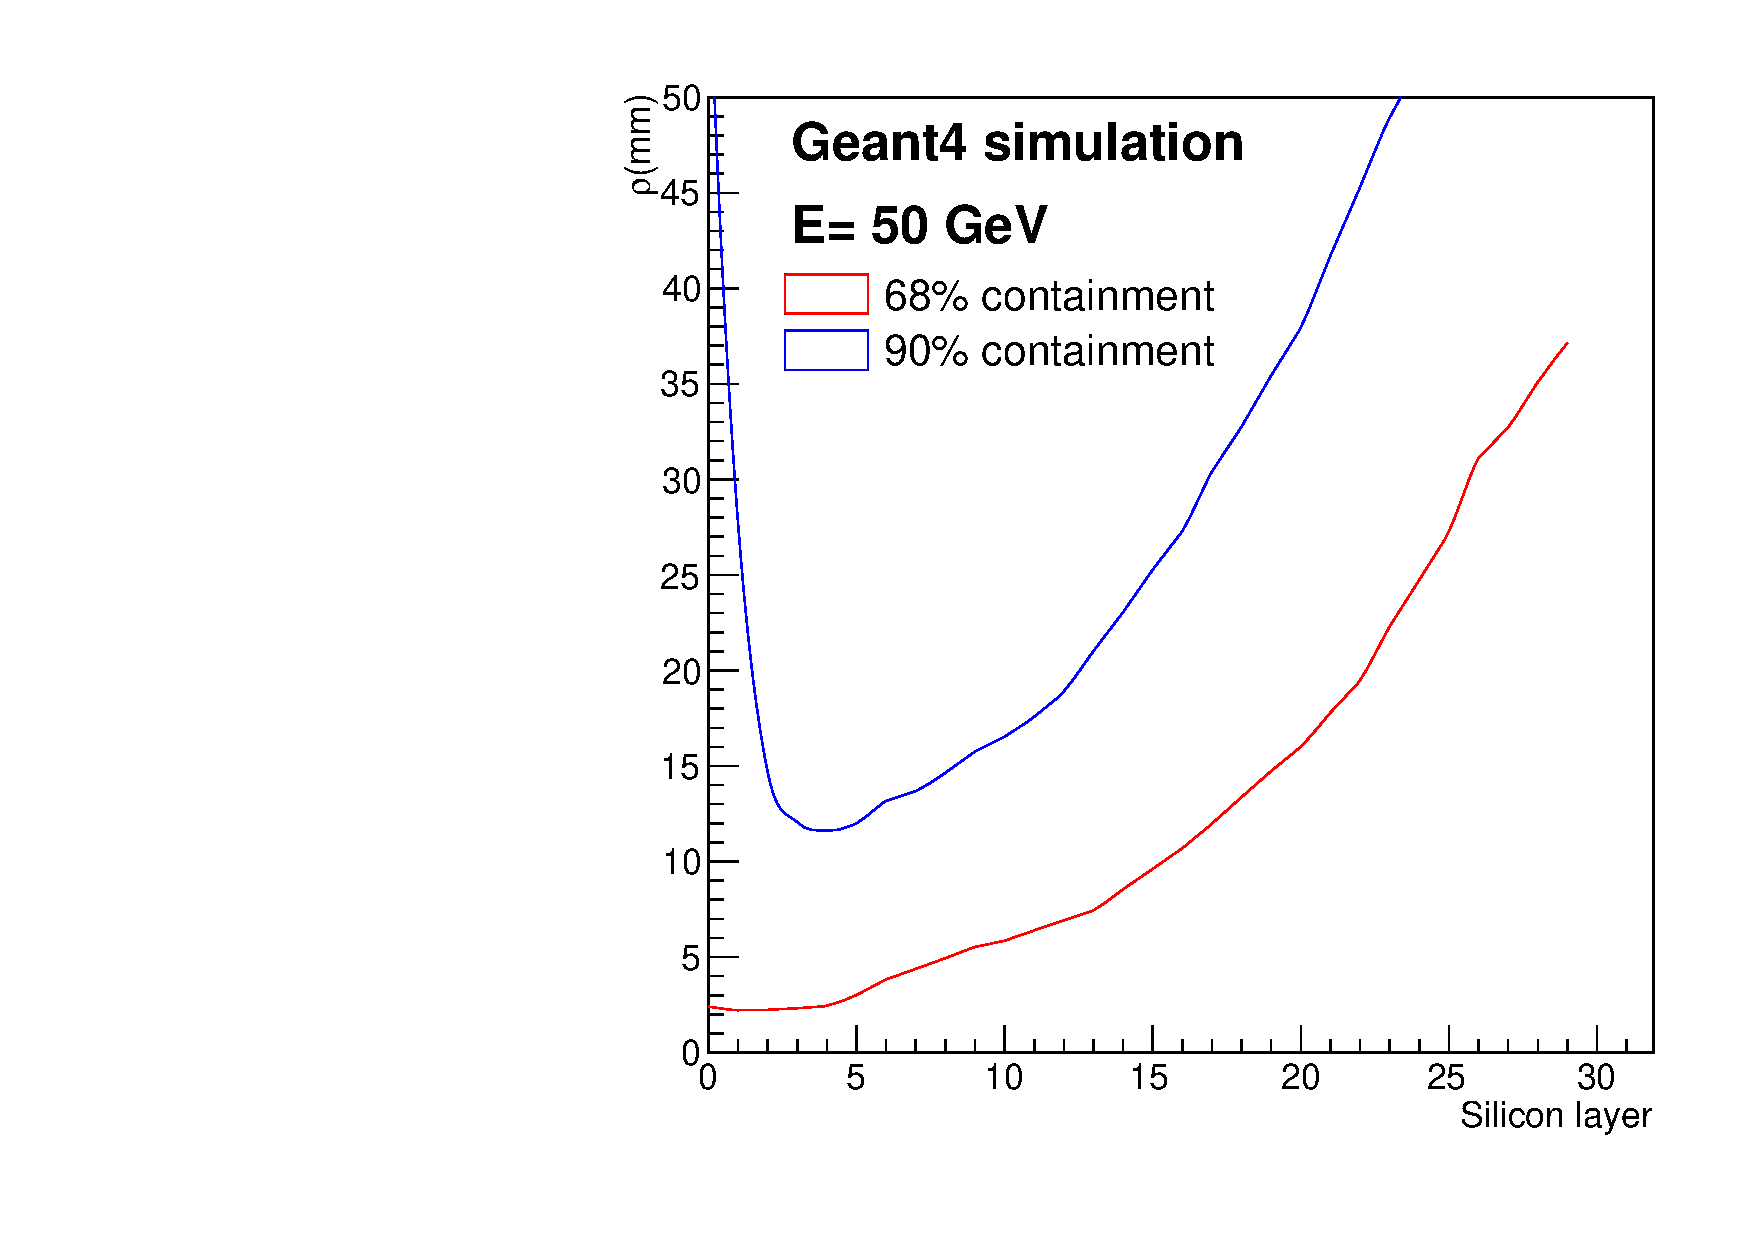
\includegraphics[width=0.24\textwidth]{figures/cmolsensorenhitsvsrE50}
    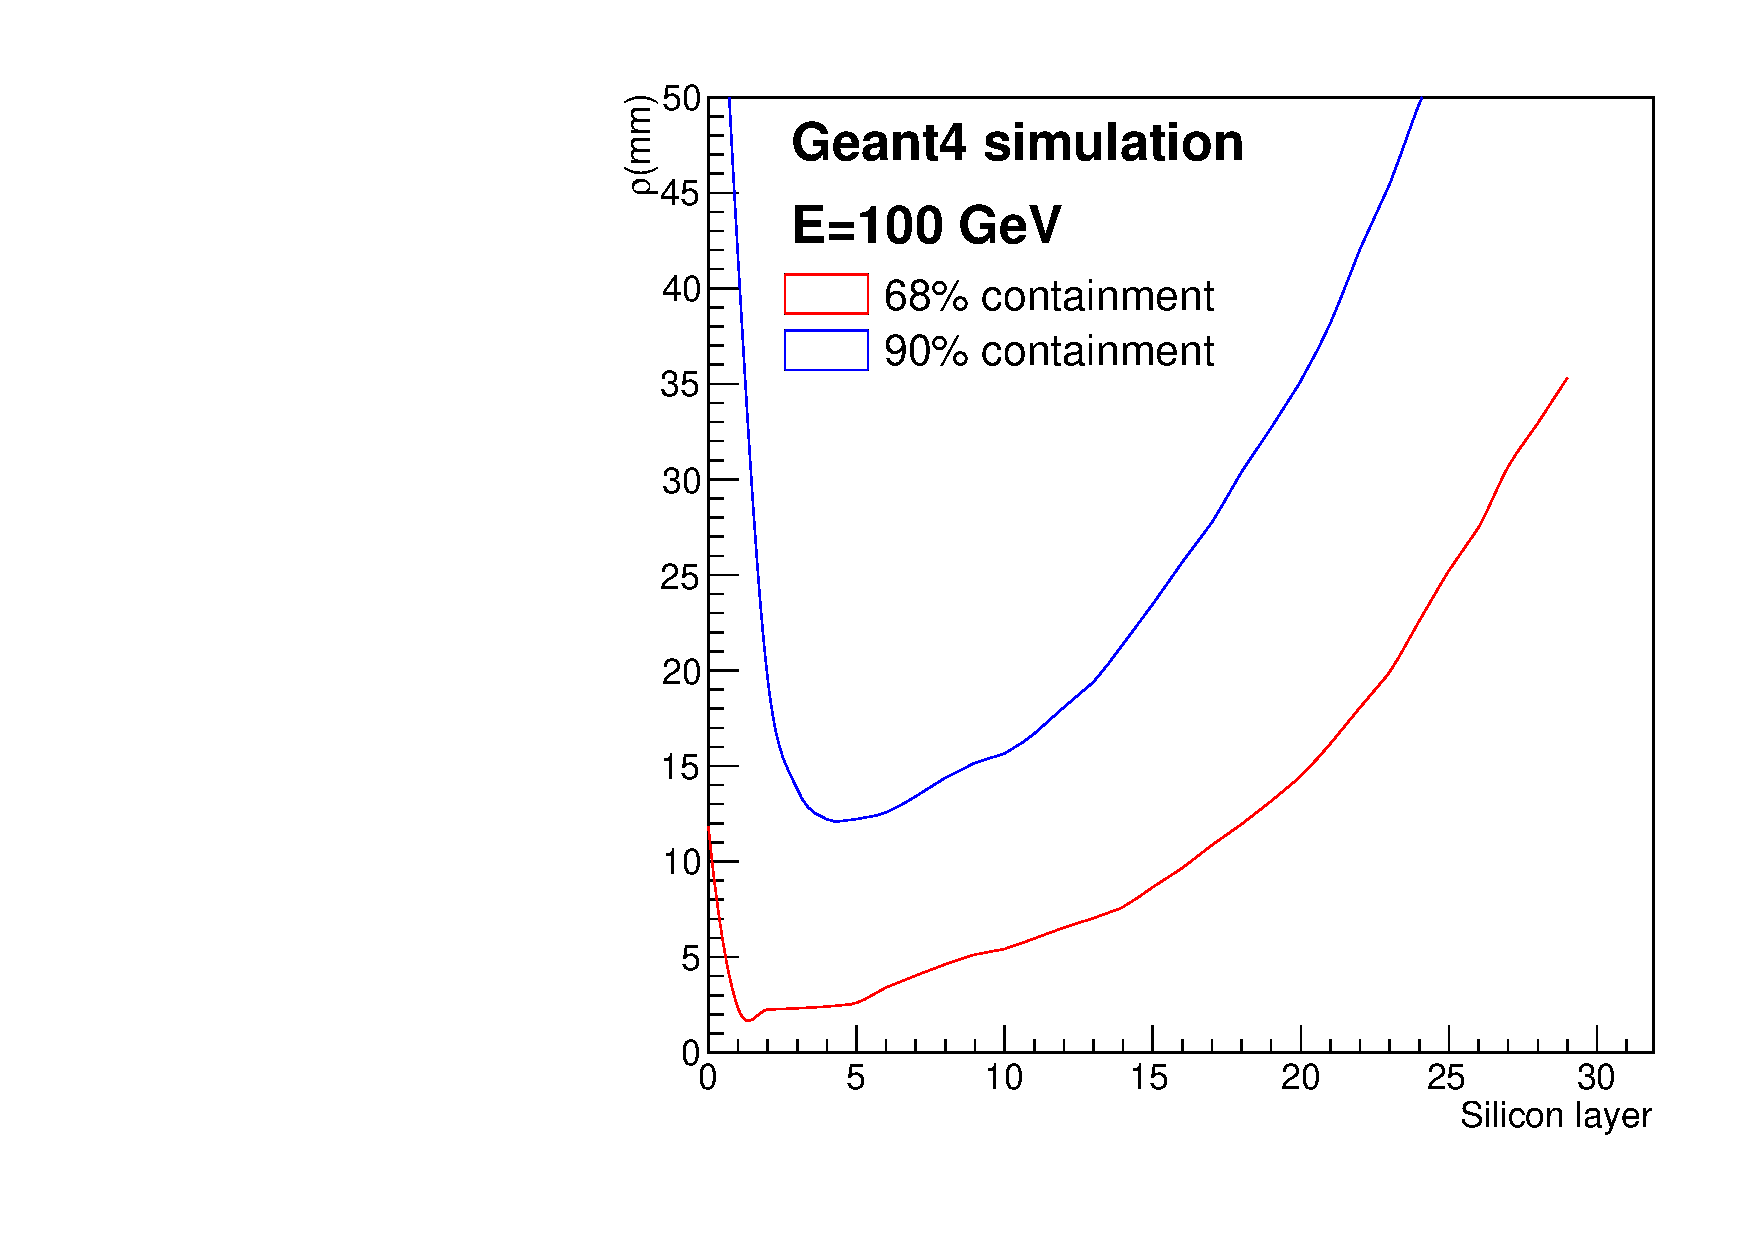
\includegraphics[width=0.24\textwidth]{figures/cmolsensorenhitsvsrE100}
    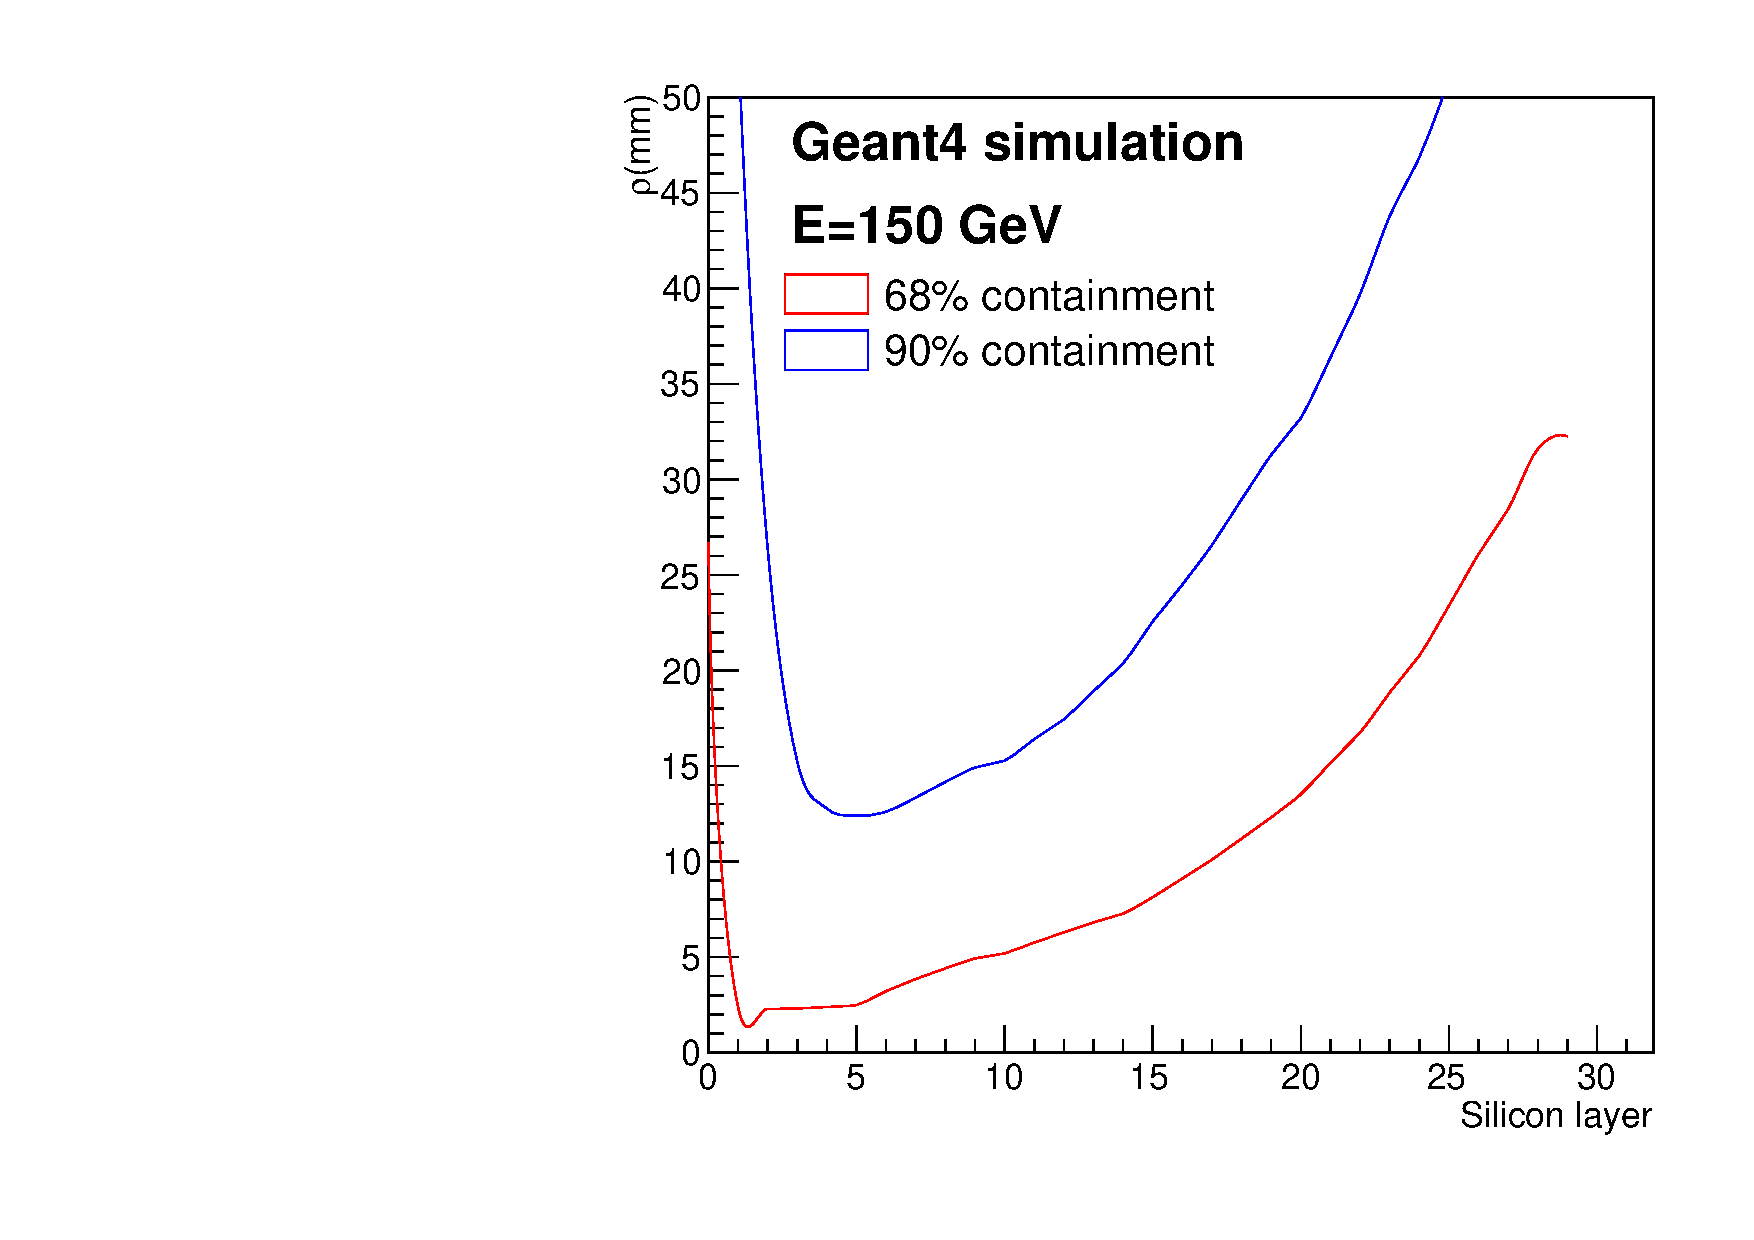
\includegraphics[width=0.24\textwidth]{figures/cmolsensorenhitsvsrE150}
    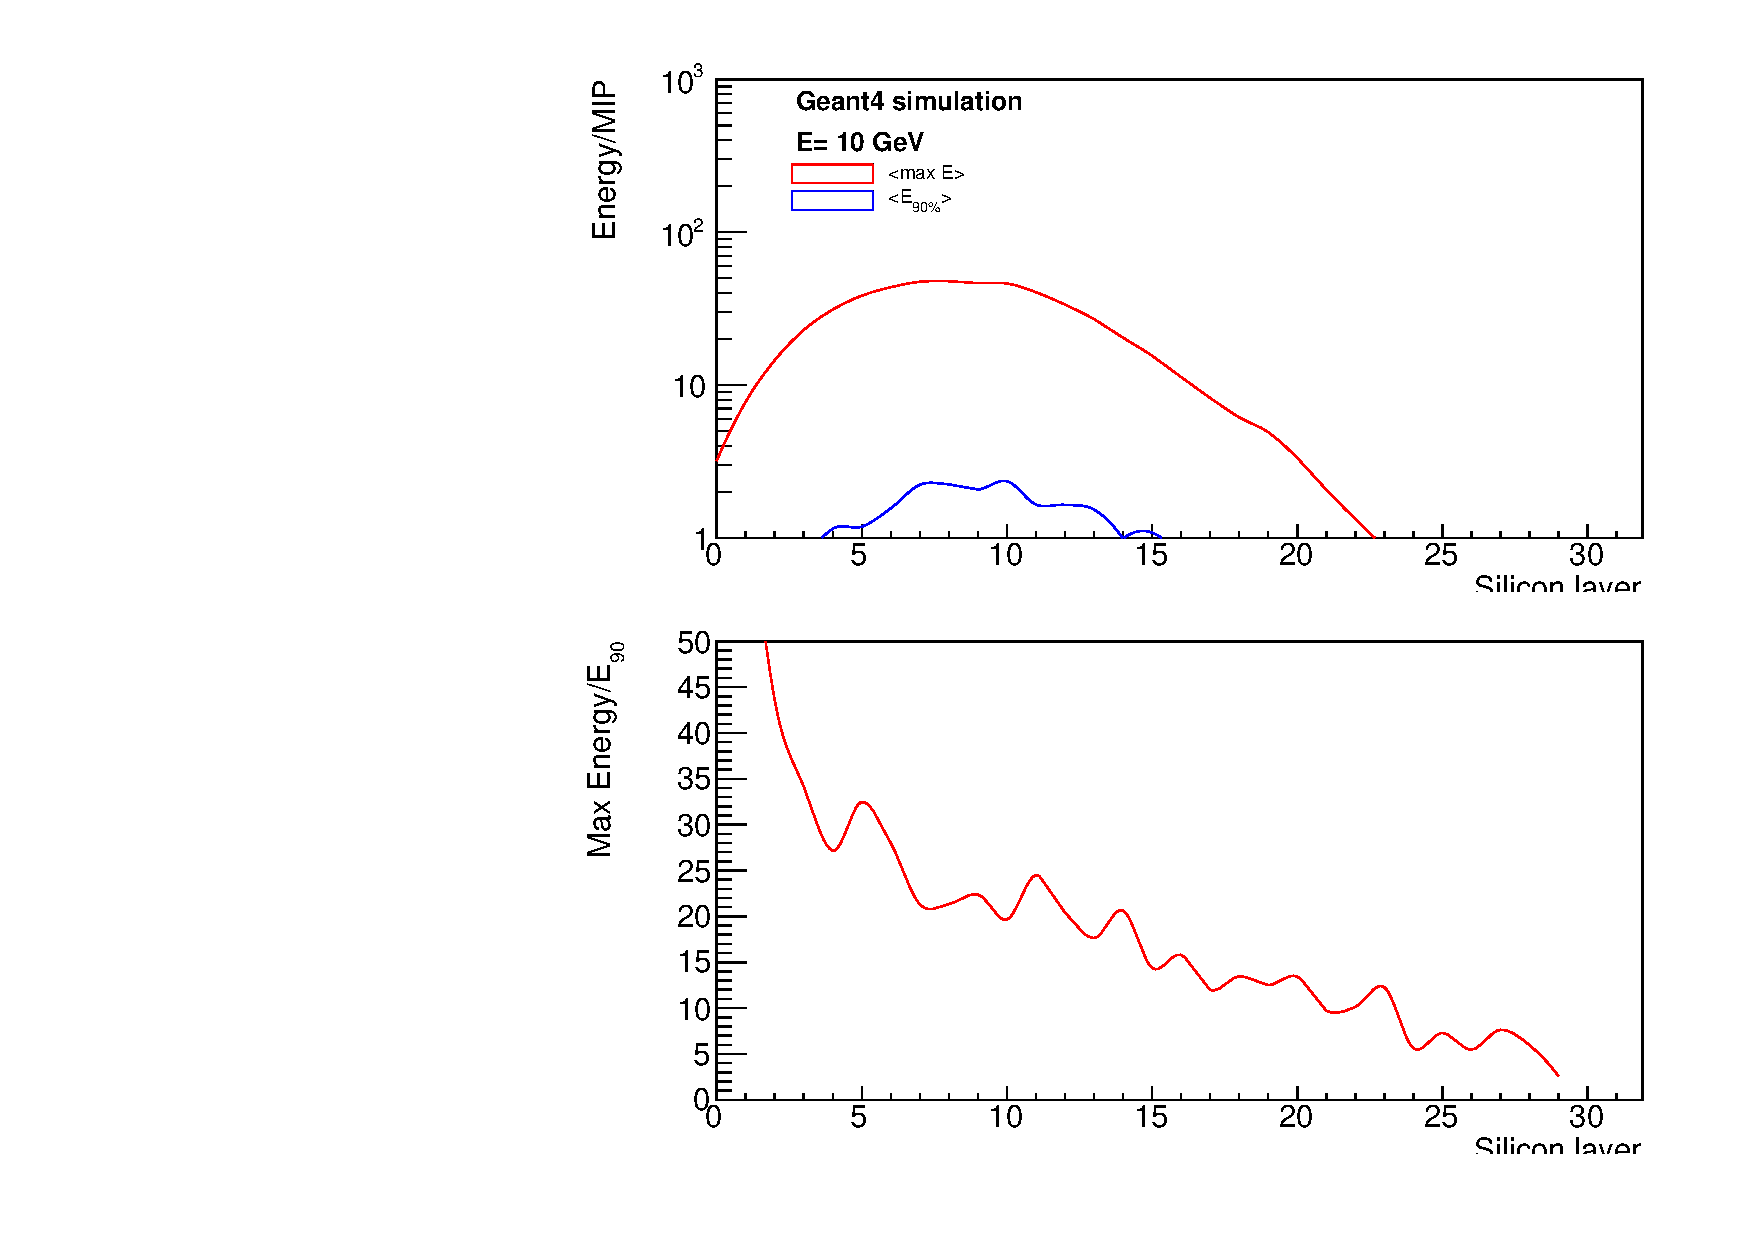
\includegraphics[width=0.24\textwidth]{figures/cdynrangesensorenhitsvsrE10}
    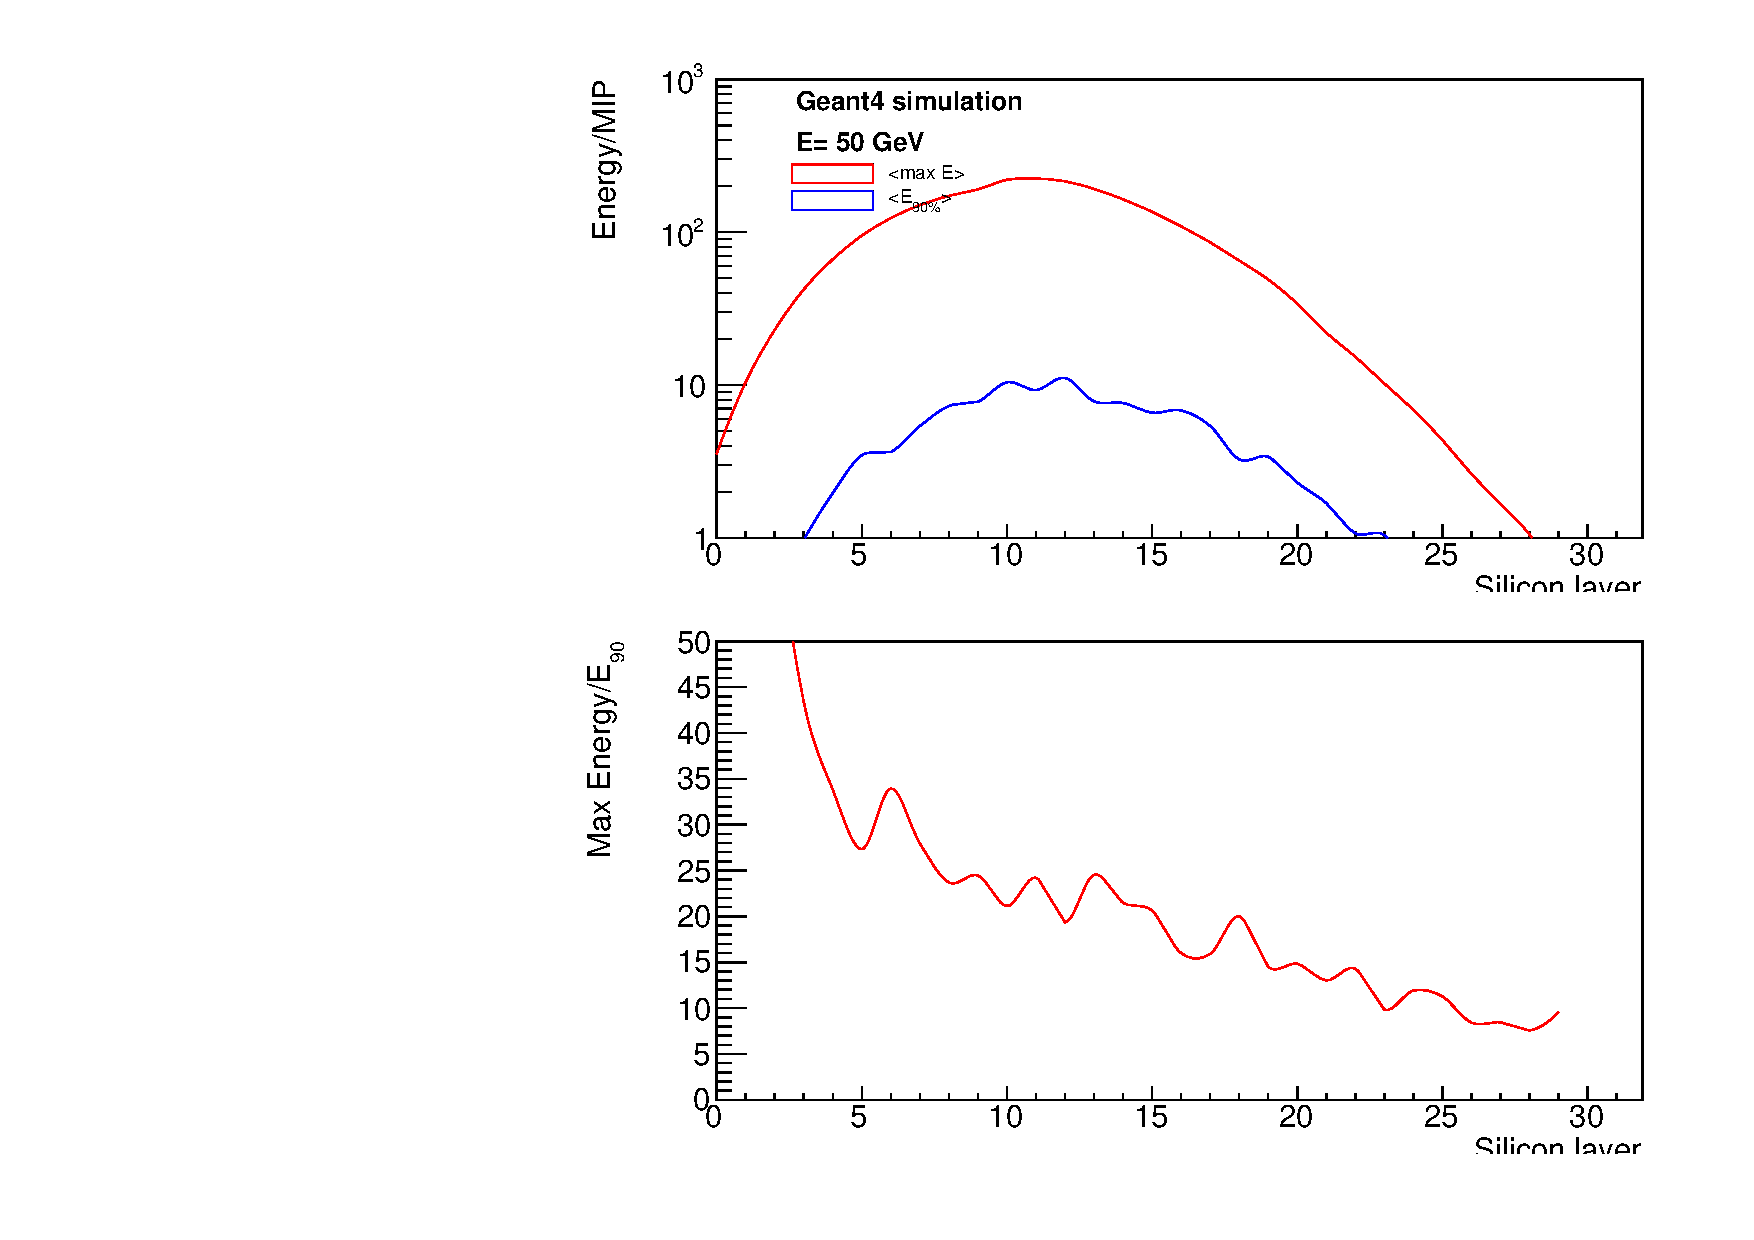
\includegraphics[width=0.24\textwidth]{figures/cdynrangesensorenhitsvsrE50}
    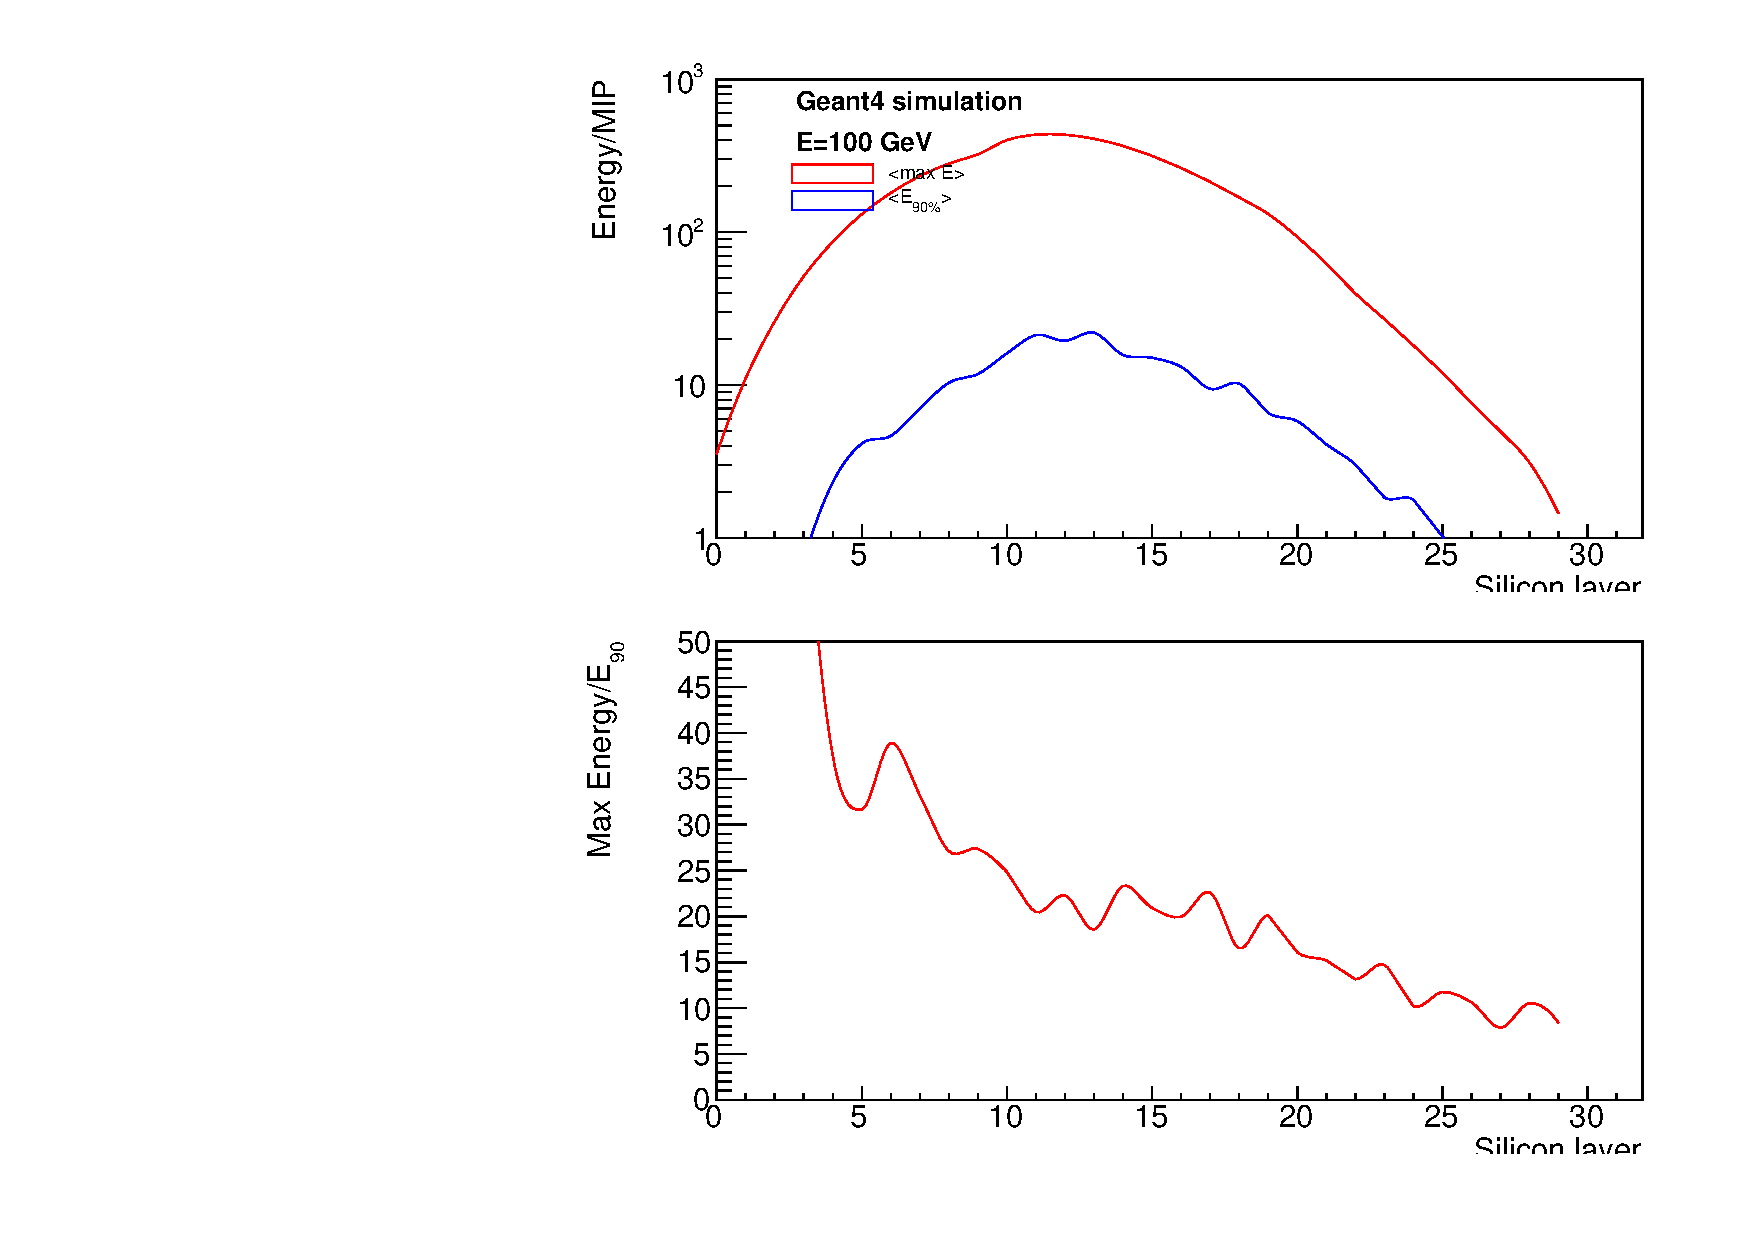
\includegraphics[width=0.24\textwidth]{figures/cdynrangesensorenhitsvsrE100}
    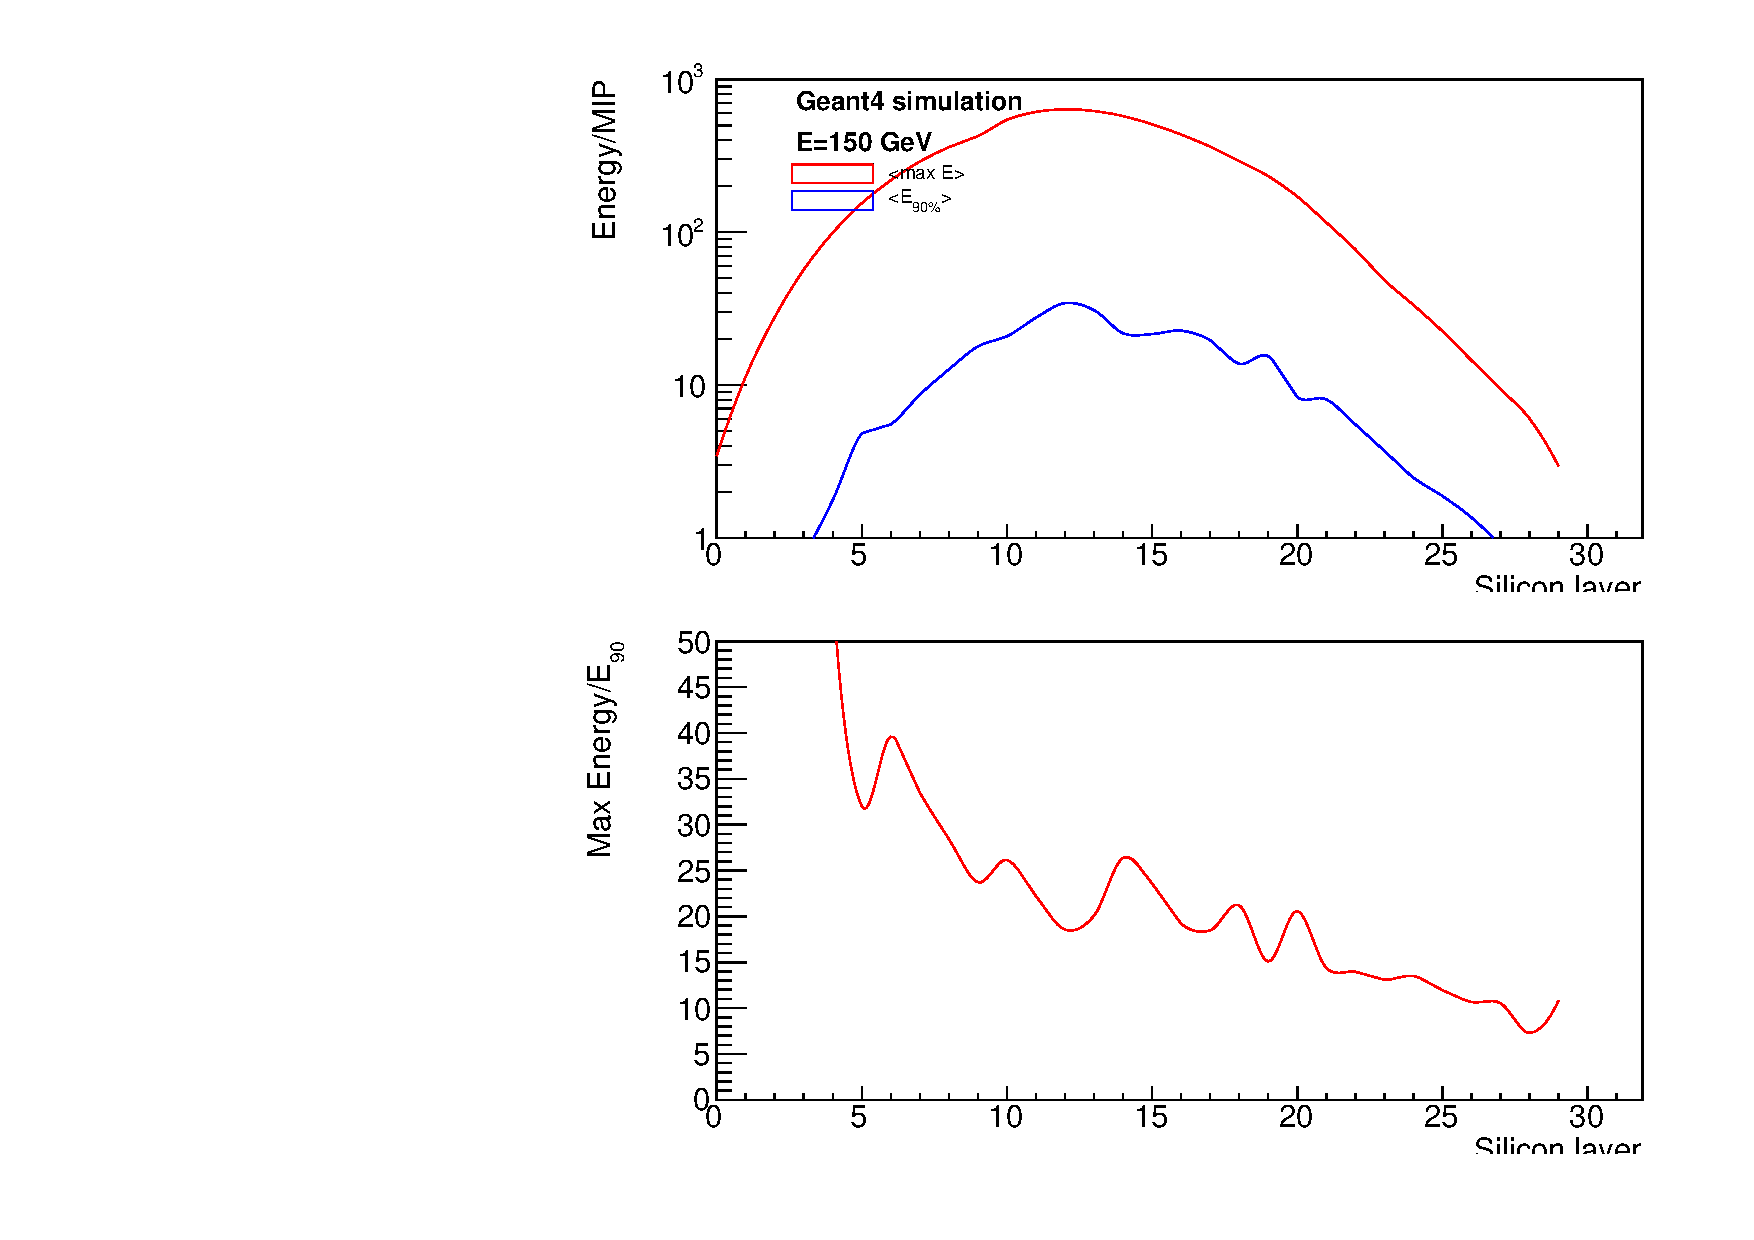
\includegraphics[width=0.24\textwidth]{figures/cdynrangesensorenhitsvsrE150}
    \caption{
{\em Top}: evolution of the distances expected to contain 68\% (blue) and
90\% (red) of the shower energy, as function of the Si layer.
{\em Bottom}: evolution of the average maximum energy deposited in
each Si layer (red) and the average energy expected to be deposited at
the 90\% containment radius. The bottom panel shows the ratio between
the two energy ranges.
From {\em left} to {\em right} incident electron energies of 10, 50,
100 and 150\GeV are shown.
   }
    \label{fig:showertranssummary}
  \end{center}
\end{figure}


From these results the Moli\`{e}re radius can be extracted, \ie the
distance at which 90\% of the shower energy is expected to be
contained. Figure~\ref{fig:showermoliere} summarizes the
result obtained.
We estimate the  Moli\`{e}re radius to be 25.5\mm
and the 68\% containment radius to be 8.5\mm.
If the air gap is increased to 4\mm (decreased to 1\mm) in the
simulation the Moli\`{e}re radius is expected to increase to 31\mm (decrease to
22\mm) and the 68\% containment radius is expected to increase to 10.5\mm
(decrease to 7\mm).
This yields a rate of the increase of the Moli\`{e}re radius
of 2.9\mm per 1\mm of Air increased and a limit of 19.3\mm
when no Air gap is present.


\begin{figure}[h!]
  \begin{center}
    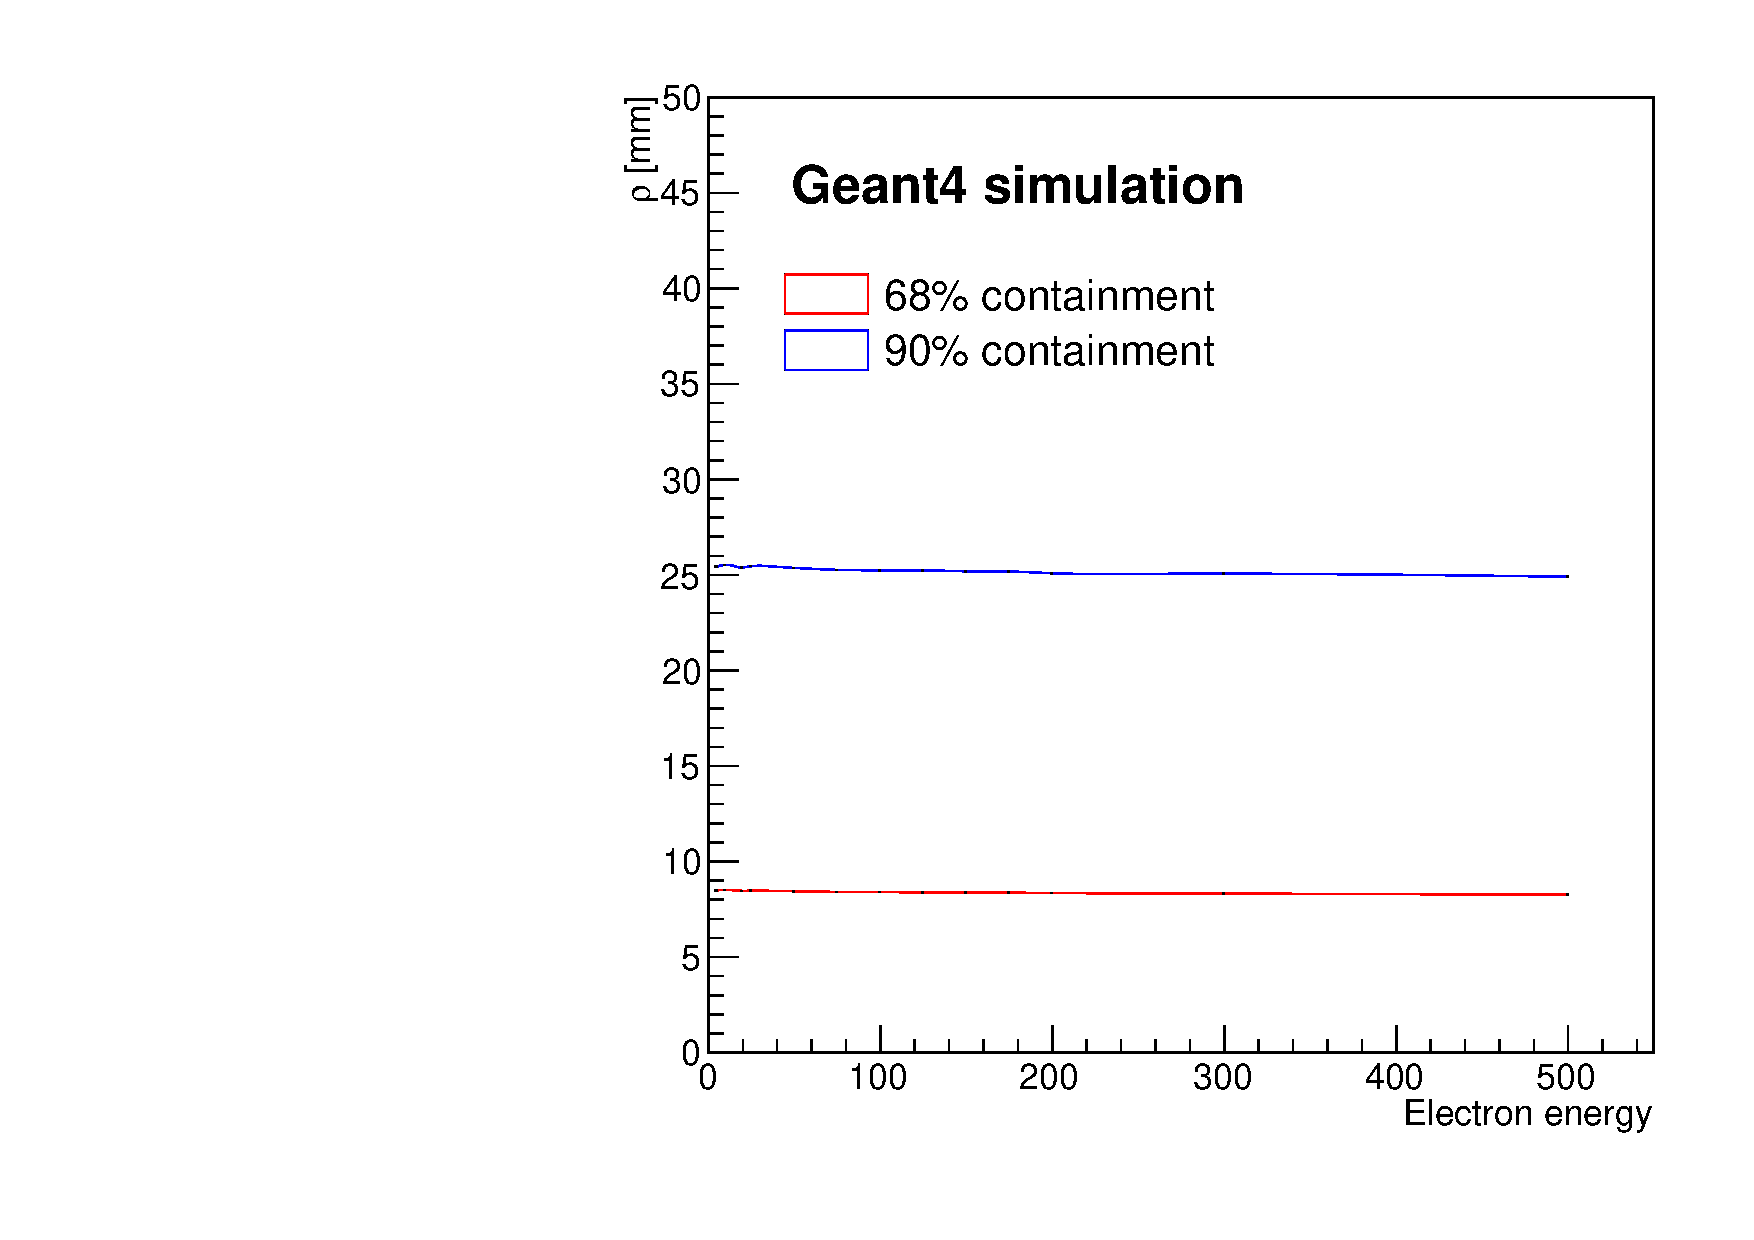
\includegraphics[width=0.6\textwidth]{figures/cmolsensorenhitsvsr}
    \caption{ Estimated Moli\'{e}re radius and radius for 68\%
      containment of the electromagnetic shower energy.}
    \label{fig:showermoliere}
  \end{center}
\end{figure}

We conclude this section with a study on the expected impact on
resolution from using isolated energy sums.
For this purpose we count only the hits which fall within a distance
$\rho$ of the shower center. The weighted energy estimator is obtained
as described in the previous Section and the resolution of this
estimator is evaluated in the same way.
Table~\ref{tab:isoresol} summarizes the expected stochastic and
constant terms of the resolution model when different radius are used.
In the extreme case where only one single $2.5\times2.5\mm^2$ cell is
used the stochastic term is expected to be degraded by 34\%.
In a more realistic scenario where a range corresponding to the
Moli\`{e}re radius is used this degradation is only 3\%.
An intermediate approach, using a dynamical range where the first layers are integrated with
smaller cone sizes and latter layers are integrated with larger cone,
sizes following the expression $8.7\times e^{0.064\times {\rm layer}}$
is expected to lead to a degradation on the resolution of the order of 9\%.
These approaches will be explored in more detail in the presence of pileup.

\begin{table}[h!]
 \begin{center}
\caption{\label{tab:isoresol} 
Electron energy resolution parameters for different radius of energy
integration. See text for details.
}
\begin{tabular}{lcc}
\hline
$\rho$ (\mm) & $\left(\frac{\sigma_{\rm E}}{\rm E}\right)_{\rm stoch}$ & $\left(\frac{\sigma_{\rm E}}{\rm E}\right)_{\rm cte}$ \\
\hline\hline
$\infty$ & $0.209\pm0.001$ & $0.0056\pm0.0001$\\
2.5 & $0.280\pm0.001$ & $0.0130\pm0.0001$\\
7 & $0.237\pm0.001$ & $0.0090\pm0.0001$\\
25 & $0.216\pm0.001$ & $0.0069\pm0.0001$\\
dynamical & $0.228\pm0.001$ & $0.0128\pm0.0001$\\
\hline
\end{tabular}
\end{center}
\end{table}